\documentclass[a4paper, oneside]{memoir}

\setlength{\overfullrule}{5pt} % Make overfull hboxes more visible

\let\emph\relax % there's no \RedeclareTextFontCommand
\DeclareTextFontCommand{\emph}{\scshape\em}

% Headers and footers
\makepagestyle{uogruled}
\makeheadrule{uogruled}{\textwidth}{\normalrulethickness}
\makefootrule{uogruled}{\textwidth}{\normalrulethickness}{\footruleskip}
\makeevenhead{uogruled}{}{\small\itshape\leftmark}{}
\makeoddhead{uogruled}{\small\itshape\rightmark}{}{\thepage\ of \totalpages}
\makeoddfoot{uogruled}{\scshape Graduate Apprenticeship Software Engineering}{}{\scshape Connor M\textsuperscript{c}Laughlin}
\makepsmarks{uogruled}{
    \nouppercaseheads{}
    \createmark{chapter}{both}{shownumber}{Chapter\ }{. \ }
    \createmark{section}{both}{shownumber}{Section\ }{. \ }
    \createplainmark{toc}{both}{\contentsname}
    \createplainmark{lof}{both}{\listfigurename}
    \createplainmark{lot}{both}{\listtablename}
    \createplainmark{bib}{both}{\bibname}
    \createplainmark{index}{both}{\indexname}
    \createplainmark{glossary}{both}{\glossaryname}
}
\pagestyle{uogruled}

\usepackage{amsmath} % Math equations
\newcommand{\Z}{\mathbb{Z}}%
\newcommand{\U}{\mathbb{U}}%
\newcommand{\R}{\mathbb{R}}%
\newcommand{\N}{\mathbb{N}}%
\newcommand{\Q}{\mathbb{Q}}%

\usepackage{bookmark} % PDF bookmarks for hyperref link
\usepackage{booktabs} % Better looking tables
\usepackage[RPvoltages]{circuitikz} % Circuit diagrams
\usepackage{cleveref}

% Make bullet points smaller and reduce the spacing between items
\usepackage{enumitem}
\setlist{itemsep=0.2\itemsep}
\renewcommand\labelitemi{\(\vcenter{\hbox{\tiny\(\bullet\)}}\)}

% Add "Contents" chapter-style title to toc, set depth of primary to section level only
\usepackage{etoc}
\etocmulticolstyle[1]{\chapter*{\contentsname}}
\etocsettocdepth{section}
\cftpagenumbersoff{chapter} % Turn off page numbers for chapter

% \usepackage{etoolbox}

\usepackage{float} % Used to force listings to have H placement

% \usepackage[T1]{fontenc}

% Reduce margins
\usepackage{geometry}
\geometry{textwidth=15.75cm, textheight=23.4cm, marginratio={5:5,5:7}}

% Make all links blend in to regular text colour
\usepackage{hyperref}
\hypersetup{
    colorlinks,
    citecolor=black,
    filecolor=black,
    linkcolor=black,
    urlcolor=black
}

\usepackage{mdframed} % Create framed boxes
\usepackage{microtype} % Slightly better text layouts
\usepackage{minted} % Code

% Palatino fonts
\usepackage{newpxtext}
\usepackage{newpxmath}

\let\attribute\relax % something else conflicts, this is a hack
\usepackage[simplified]{pgf-umlcd} % Used to have UML diagrams

\usepackage{pifont}
\newcommand{\cmark}{\ding{51}}%
\newcommand{\xmark}{\ding{55}}%

\usepackage[binary-units=true]{siunitx} % Units
\usepackage{tabularx} % Column types

\usepackage{tcolorbox} % The note box
\tcbuselibrary{minted,breakable,skins}

\usepackage{tikz}
\usetikzlibrary{backgrounds, er, fit, intersections, positioning, through}

\usepackage[page]{totalcount}

% Off white and off black are nicer on the eyes
\usepackage{xcolor}
\pagecolor{gray!10}
\color{black!90}

\setminted{bgcolor=white, framesep=2mm}
\renewcommand{\theFancyVerbLine}{\large \oldstylenums{\arabic{FancyVerbLine}}}

% Number all the way to subsections
\setsecnumdepth{subsubsection}

% % Chapter Headers
\chapterstyle{verville}
\setsecheadstyle{\LARGE\boldmath\scshape\bfseries} % large bold small caps
\setsubsecheadstyle{\large\scshape\boldmath\bfseries\raggedright} % large bold small caps
\setsubsubsecheadstyle{\itshape\bfseries} % bold italic

\newtcolorbox[blend into=figures]{highlight}[1]{
   float=htb,
   title={#1},
   every float=\centering,
   colframe=black,
   arc=0.5mm,
   colback=white,
   boxrule=0mm,
   width=0.95\linewidth,
   valign=center,
   left=7.5mm,
   right=7.5mm,
   top=0mm,
   bottom=0mm,
   after upper={\centering},
   after={\noindent}
}

\newtcolorbox[auto counter,number within=section]{note}{
   breakable,
   center,
   title=Note.~\thetcbcounter,
   colframe=black,
   arc=0.5mm,
   left=7.5mm,
   right=7.5mm,
   colback=white,
   boxrule=0mm,
   width=0.95\linewidth,
   valign=center,
   after={\noindent}
}

\newenvironment{code}[1]
{%
  \VerbatimEnvironment%
  \begin{minted}[linenos,numbersep=5pt,frame=lines,framesep=2mm,autogobble]{#1}%
}{%
  \end{minted}
}

\begin{document}

\frontmatter

\title{Glasgow University Software Engineering Graduate Apprenticeship}
\date{\today}
\author{Connor M\textsuperscript{c}Laughlin\\
{\begin{tabularx}{0.85\textwidth}{*{3}{>{\medskip\small\centering\arraybackslash}X}}
    Derek Sommerville & Matthew Barr & Waqar Nabi
\end{tabularx}}
}
\maketitle
\newpage

\renewcommand{\cftsectionfont}{\small}

\tableofcontents

\renewcommand{\cftchapterfont}{\bfseries}
\renewcommand{\cftsectionfont}{\large\bfseries}
\renewcommand{\cftsubsubsectionfont}{\small\itshape}

\newpage
\listoffigures

\mainmatter{}

\part{Semester One (2020-11-02)}
\chapter{How To Learn A New Language}
\section{Session One}\label{sub:session_one}


\subsection{Sprint One}\label{ssub:sprint_one}

\begin{itemize}
	\item First half is variables, loops and other basic programming constructs
	\item The second half is more advanced with object oriented programming
\end{itemize}

\begin{note}
	Note: Overall the course could seem very easy, by Christmas, though, it will not.
\end{note}

\subsection{The Workplace}\label{ssub:the_workplace}

When back in the workplace, we will get tasks, don't stress about these too much --- if work deadlines are too tight, don't worry.
Learning logs will be useful for report writing.
You should take note of examples of university work found will at work.

Barclay's people are all just doing busy work --- nobody has done any programming yet and they started in August 2020. Because of this, my team all have no programming experience making me the designated experienced developer.

\section{Session Two}\label{sub:session_2_types}

\subsection{Types}\label{ssub:types}

\emph{Primitive types} are ones that cannot be broken down (\mintinline{c}{int}, \mintinline{c}{char}, \mintinline{c}{long}).
\emph{Composite types} can be broken down (array, class and sometimes strings are \mintinline{c}{char[]}s)

\begin{note}
	\begin{itemize}
		\item[Note:] In most old languages (like C, C++), booleans are often represented by just a \(1\) or  \(0\).
		\item[] Strings are often just stored as an array of ASCII codes, Python is an exception where \mintinline{c}{chars} are just strings with length 1
	\end{itemize}
\end{note}

\subsection{Learning Logs}\label{ssub:learning_logs}

A final workplace report worth \(25\%\) is due 2021-03-01.
\begin{itemize}
	\item Reflect and show what was learned at work.
	\item Should be about \(1500\) words in length.
	\item Should include a critical evaluation of the programming practices encountered.
	\item Should include examples of programming concepts covered in HTLANL (inheritance, scope, etc.).
	\item \textbf{What have I learned?}
\end{itemize}

\subsection{Academic Writing}\label{ssub:academic_writing}

On Moodle there is a basic introduction, phrase bank and a like to LEADS (a university program to help with academic writing).

Reflective writing is evidence of reflective thinking.
Reflective thinking helps to reinforce what we have learned.

Reflective writing is generally a more relaxed form of writing where you can write in first person (I, me, we).

Reflective writing should aim to look back at an event (\emph{description}), analyse and explain the event (\emph{interpretation}) and decide what this means for me in the future (\emph{outcome}).

\begin{note}
	\begin{itemize}
		\item [Note:] When describing a theory or model, use present tense since the theory or model is still the same.
		\item[] When talking about events, use past tense since the events happened in the past.
	\end{itemize}
\end{note}

\section{Section Three}\label{sub:section_three}

\subsection{Statements}\label{ssub:statements}

Statements are sequences of code that do something.
A program is a sequence of statements.
All expressions (\mintinline{python}{1+1}) are valid statements.

Assignment statements are a special type of statement:

\begin{itemize}
    \item They bind a value to a name.
    \item They bind the right hand side value to the left hand side value.
    \item Usually \mintinline{python}{=} symbol is used, but some languages use \mintinline{pascal}{:=} (Pascal) and \mintinline{r}{<-} (R).
\end{itemize}

\subsubsection{Expressions}\label{ssub:expressions}

Expressions don't necessarily have to have any effect.

\begin{itemize}
    \item \mintinline{python}{x + 5}
    \item \mintinline{python}{fn(32 * age) > 0}
\end{itemize}

\subsubsection{Operators}\label{ssub:operators}

Operators do a thing to a variable.
They are used in format: operand, operator, operand and they can often do different things in different contexts.

\subsubsection{Mathematical operators}\label{ssub:mathematical-operators}

\begin{itemize}
    \item \mintinline{python}{+}, \mintinline{python}{-}, \mintinline{python}{*}, \mintinline{python}{/}
    \item \mintinline{python}{**} and \mintinline{haskell}{exp} are for powers
    \item \mintinline{c}{%}, \mintinline{haskell}{rem} and \mintinline{haskell}{mod} are for modulus (remainder)
\end{itemize}

\subsubsection{Boolean Operators:}\label{ssub:boolean-operators}

\begin{itemize}
    \item \mintinline{python}{not} flips the expression
    \item \mintinline{python}{or} evaluates \mintinline{java}{true} if either operand is \mintinline{java}{true}.
    \item \mintinline{python}{and} evaluates \mintinline{java}{true} if both operands are \mintinline{java}{true}.
\end{itemize}

\subsubsection{Operator Overloading}\label{ssub:operator-overloading}

\begin{itemize}
    \item One operator can have different meanings depending on context:
        \begin{itemize}
            \item \mintinline{python}{"5" + "6" = "56"}
            \item \mintinline{python}{5 + 6 = 11}
        \end{itemize}
    \item Most languages don't allow the creation of custom overloaded operators (C is a notable exception)
\end{itemize}

\subsubsection{Precedence}\label{ssub:precedence}

\begin{itemize}
    \item Largely follows BODMAS
        \begin{minted}{python}
            x = 2 + 3 * 4
            x = 2 + 12
            x = 14
        \end{minted}
\end{itemize}

\subsection{Typing}\label{sub:typing}

Before an operator's operation can be performed, the type must be known.
Some type checkers happen at runtime, others at compile time depending on language.

\subsubsection{Static Typing}\label{ssub:static-typing}

\begin{itemize}
    \item A variable only ever has one type (a \mintinline{c}{long} will always be a \mintinline{c}{long}).
    \item Types can be set or inferred by the compiler.
    \item All operands and types are checked at compile time
\end{itemize}

\subsubsection{Dynamic Typing}\label{ssub:dynamic-typing}

\begin{itemize}
    \item Variables have no type, so values (which do have types) can be assigned to any variables.
    \item Operands and types are checked at runtime.
\end{itemize}

\subsubsection{Duck Typing}\label{ssub:duck-typing}

\begin{itemize}
    \item ``If a value looks like a certain type, acts like a certain type and talks like a certain type, then it is that type.''
    \item The language tries to do exactly what the programmer asks with the data given.
\end{itemize}

\subsubsection{Errors}\label{sub:errors}

\begin{itemize}
    \item You can only ever compare two comparable types. For example, in Python: \mintinline{python}{1 < True == False}.
\end{itemize}

\subsubsection{Type Conversions}\label{ssub:type-conversions}

\begin{itemize}
    \item Implicit:
        \begin{itemize}
            \item Happens automagically depending on context.
            \item For example: \mintinline{c}{int num = 123456789; long big = num}
        \end{itemize}
    \item Explicit (\emph{casting}):
        \begin{itemize}
            \item The programmer manually changes the types.
            \item For example: \mintinline{python}{int(n)}, \mintinline{typescript}{n as int}, \mintinline{c}{(int)n}
        \end{itemize}
\end{itemize}

\section{Session Four}\label{sec:session_four}

\subsection{Control}\label{sub:control}

Control allows you to chose which path to follow based on conditions.
A branch is somewhere the code can follow \(>1\) path.

\subsubsection{The \mintinline{python}{if} statement}\label{ssub:the-if-statement}

\begin{itemize}
	\item The very simplest type of branching.
	      \begin{minted}{python}
            if x:
                branch_one()
            if y:
                branch_two()
        \end{minted}
\end{itemize}

\subsubsection{The \mintinline{typescript}{else if} statement}\label{ssub:the-else-if-statement}

\begin{itemize}
	\item One of the two paths are always followed.
	      \begin{minted}{python}
            if x:
                branch_one()
            else:
                branch_two()
        \end{minted}
\end{itemize}

\subsubsection{The \mintinline{python}{elif} statement}\label{ssub:the-elif-statement}

\begin{itemize}
	\item Can handle more than just two outcomes.
	\item Could also be done with just lots of \mintinline{python}{if} statements, this is nasty and hard to read.
\end{itemize}

\begin{note}
	Switch and case statements can also handle more than one branch too.
\end{note}

\subsection{Iteration}\label{sub:iteration}

Repeating code is what makes computers powerful.
The key thing about looping is you do the same thing on different data.

\subsubsection{Definite Iteration}\label{ssub:definite-iteration}

\begin{itemize}
	\item Loop a certain number of times.
	\item Usually done with a \mintinline{python}{for} keyword.
\end{itemize}

\subsubsection{Nested Loops}\label{ssub:nested-loops}

\begin{itemize}
	\item One loop inside of another.
	\item Too many levels of looping is hard to read and slow.
\end{itemize}

\subsubsection{Indefinite Iteration}\label{ssub:indefinite-iteration}

\begin{itemize}
	\item Continues until some condition is met.
	\item Usually done with the \mintinline{python}{while} keyword.
	\item If the condition is \mintinline{java}{true}, the loop continues, otherwise it stops.
	\item Generally worse than definite loops.
	\item Use indefinite loops only when you don't know how many iterations there will be.
\end{itemize}

\section{Session Five}\label{sec:session_five}

\subsection{Subprograms}\label{sub:subprograms}

A \emph{subprogram} is a sequence of statements that can be called more than once (they are named blocks of code).
Subprograms often return a value which allows the subprogram to give feedback.
Sometimes these are called \emph{subroutines}, \emph{procedures}, \emph{functions} or \emph{methods}.
Subprograms temporarily reroute the flow of execution with isolated local variables and control the flow of data with arguments and returns.

\subsubsection{Return}\label{ssub:return}

Gives control back to the calling code from any point inside a function (even half way through).
If return is skipped, execution will end at the end of the code block.

\subsubsection{Call Stack}\label{ssub:call_stack}

Most languages have a stack of calls so that it always knows where code should return to.
When a function is called, it puts the point to return to onto the stack.
When a function returns again, it pops off the function and returns back to the point.

\subsubsection{Parametrisation}\label{ssub:parameterisation}

Functions are only really useful if they can be called with different data.
This is why we parametrise the functions to send data from the calling code.
\emph{Parameters} are the received data.
\emph{Arguments} are passed in.
Parameters are always required, but may be given a default value so they aren't need to be passed in every time.

\subsubsection{Why do we use functions?}\label{ssub:why_do_we_use_functions_}

\paragraph{Decomposition}\label{par:decomposition}

Makes code more readable and manageable.

\paragraph{Isolation}\label{par:isolation}

Isolate variables used in one chunk from those in another.

\paragraph{Abstraction}\label{par:abstraction}

Create a general function that can be used in many places for different problems.

\paragraph{Laziness}\label{par:laziness}

They can eliminate boring, repetitive tasks.
This is sometimes called \emph{generalisation} and is often done through abstraction. % link here

\paragraph{Remove repetition}\label{par:remove_repetition}

Repetition makes it very easy to make copy-paste mistakes and makes code harder to read.

\paragraph{Code sharing}\label{par:code_sharing}

Code in functions is far easier to share with other people if it is in chunks already.

\paragraph{Control the Effects}\label{par:control_the_effects}

Code in functions only affects local variables so there is a smaller risk of it breaking something outside.

\section{Session Six}\label{sec:session_six}

\subsection{Work-based Task}\label{sub:work_based_task}

Ask someone how they go about learning a new programming language or learning something new about a language they already know.

\subsection{Scope}\label{sub:scope}

Creating new variables inside of functions creates ones that are only available inside of that function named \emph{local variables}.
``Each function has its own workspace.''
Local variables are not persisted across calls.

\subsubsection{Global Scope}\label{ssub:global_scope}

These are variables outside of a function which are visible to all code.
Some languages don't really have global variables (C\# and Java just have \mintinline{java}{static}) and in Python, globals are read only by default to protect from accidental writes in local scopes (use \mintinline{python}{global} to write to them).

\subsubsection{Shadowing}\label{ssub:shadowing}

Local variables can shadow a global making it inaccessible.
In Python \mintinline{python}{global} must be used to edit globals in local scopes.

\subsubsection{Evils of Globalisation}\label{ssub:evils_of_glovalisation}

\emph{Globalisation} is generally considered bad practice because it makes functions rely on each other and variables can be changed accidentally leading to unintended behaviour.

\subsection{Recursion}\label{sub:recursion}

\emph{Recursion} is when a function calls itself.
This is an alternative to \mintinline{python}{while} and \mintinline{python}{for} loops.
Some problems can be solved by calling the same function on the data returned from last time.
eg. Fibonacci sequences, fractals, binary trees, sorts.


\section{Session Seven}\label{sec:session_seven}

\subsection{Data Structures}\label{sub:data_structures}

Organising data into structures is important.
Most languages have many built in data structures.
\emph{Data structures} are sometimes called \emph{composite data types} instead.
eg. Lists (arrays), dictionaries (hash maps), tuple (records).

\subsubsection{Lists (Python)}\label{ssub:lists_python_}

Python lists are dynamically sized meaning elements can be added or removed without changing the size unlike in C, for example, where an array has a fixed size.
Python lists are dynamically typed meaning that one list can have many different types of data.
The literal syntax (\mintinline{python}{a = [1, 2, 3, 4, 5, 6]}) can be used to declare and initialise a list in one line.

The \mintinline{python}{len()} function will return the number items in a list. eg. \mintinline{python}{len([1, 2, 3, 4, 5, 6]) == 6}.

To access an individual element in the list, use the \mintinline{python}{items[index]} syntax.
Lists can also be iterated over using a \mintinline{python}{for} loop: \mintinline{python}{for element in items}.

The index counts from \(0\) and maximises at \mintinline{python}{len(items) - 1}.
Python supports negative indexing (\mintinline{python}{items[-1]}) to access elements by their count from the end of the list.

All list-like objects can be sliced to make a subsequence of the original with \mintinline{python}{items[start:end:step]} which works on lists, strings, tuples, etc.
All list-like objects can also be added together to create a new list-like object that combines the two operands.

For lists, \mintinline{python}{items.append(element)} can also be used to add items, with \mintinline{python}{items.remove(element)} removing the first instance of \mintinline{python}{element}.


\section{Section Eight}\label{sec:section_eight}

\subsection{Lists (Python) cont.}\label{sub:lists_python_cont_}

\begin{note}
    \begin{itemize}
        \item[Note:] Never alter an array or list while iterating over it.
    \end{itemize}
\end{note}

\paragraph{Lists as stacks}\label{par:lists_as_stacks}

Use \mintinline{python}{items.pop()} to remove and return the last item from the list.

\paragraph{Lists as queue}\label{par:lists_as_queue}

Use \mintinline{python}{items.pop(0)} to remove and return the first item in the list.

\paragraph{Membership testing}\label{par:membership_testing}

This is checking whether a data structure contains a value.
Use the Python \mintinline{python}{in} operator.
eg. \mintinline{python}{element in items}

\paragraph{Finding elements}\label{par:finding_elements}

Use \mintinline{python}{items.index(element)} to find the index of the \textbf{first} occurrence of \mintinline{python}{element}.

\paragraph{Counting elements}\label{par:counting_elements}

Use \mintinline{python}{items.count(element)} to return the number of occurrences of \mintinline{python}{element} there are in \mintinline{python}{items}.

\paragraph{Sorting elements}\label{par:sorting_elements}

Many different types can be sorted (\mintinline{python}{str}, \mintinline{python}{int}, etc) using the object's \mintinline{python}{__gt__()} and \mintinline{python}{__lt__()} methods.
Use \mintinline{python}{items.sort()} to sort the list in place and \mintinline{python}{sorted} to return a new sorted list.

\begin{note}
    \begin{itemize}
        \item[Note:] Lists of lists are sorted by the first element in each nested list.
    \end{itemize}
\end{note}

\paragraph{Reversing elements}\label{par:reversing_elements}

The items in a list can be reversed in several different ways:

\begin{itemize}
    \item Without sorting, returning a new list: \mintinline{python}{items[::1]}
    \item In place, with sorting: \mintinline{python}{items.sort(reverse=True)}
    \item With sorting, returning a new list: \mintinline{python}{sorted(items, reverse=True)}
\end{itemize}


\section{Session Nine}\label{sec:session_nine}

\subsection{Mutability (Lists)}\label{sub:mutability}

\emph{Mutability} describes whether or not an object can be altered after it has been initialised.
Since we can do \mintinline{python}{items.append(element)}, the list \mintinline{python}{items} is mutable.
In Python, core types (like \mintinline{python}{int}s and \mintinline{python}{str}s) are immutable, that's why \mintinline{python}{"str" + "ing"} creates a new string \mintinline{python}{"string"}.

\subsubsection{Side-effects of Mutability}\label{ssub:side_effects_of_mutability}

\begin{highlight}{The side-effects of mutability}
    \begin{code}{python}
		items = [[0]] * 3
		new_items = items
		new_items[0][0] = 1
		print(items) -> "[[1], [1], [1]]"
		print(new_items) -> "[[1], [1], [1]]"
    \end{code}
\end{highlight}

\subsubsection{Copying Lists}\label{ssub:copying_lists}

\begin{highlight}{Copying lists}
    \begin{code}{python}
		items = [1, 2, 3]
		b = a[:]
		b.append(4)
		a == b -> False
    \end{code}
\end{highlight}

\subsubsection{Testing for Equality}\label{ssub:testing_for_equality}

\noindent
Assigning means both variables are equal:

\begin{highlight}{Testing for equality}
    \begin{code}{python}
		a = [1]
		b = [1]
		a == b -> True
    \end{code}
\end{highlight}

\noindent
Copying creates an identical list:

\begin{highlight}{Copying lists}
    \begin{code}{python}
		a = [1]
		b = a[:]
		a == b -> True
    \end{code}
\end{highlight}

\noindent
Assigning just assigns a reference to the new variable, instead of making a new list:

\begin{highlight}{Reassigning lists}
    \begin{code}{python}
		a = [1]
		b = a
		a is b -> True
    \end{code}
\end{highlight}

\noindent
Copying a list creates a brand new list so they don't have the same \mintinline{python}{id()}:

\begin{highlight}{Creating a new list}
    \begin{code}{python}
		a = [1]
		b = a[:]
		a is b -> False
    \end{code}
\end{highlight}

\noindent
Since assigning just assigns the reference, the original can be altered by changing the second one:

\begin{highlight}{Altering the original list}
    \begin{code}{python}
		a = [1]
		b = a
		b.append(2)
		print(a) -> [1, 2]
    \end{code}
\end{highlight}

\subsection{Mutability (Tuples)}\label{sub:mutability_tuples_}

Tuples are immutable meaning that once have been created, they cannot be changed.
Tuples use the same syntax as lists, except with \mintinline{python}{()} instead of \mintinline{python}{[]}. eg \mintinline{python}{items = (1, 2, 3, 4)}.
Tuples are good for debugging since they cannot be changed after initialisation.
It is possible to convert lists to tuples using the \mintinline{python}{tuple(items)} command and \mintinline{python}{list(items)} to go back again.

\begin{highlight}{Mutability in tuples}
    \begin{code}{python}
		a = ("2", 3, [1, 2, 3])
		a[2] = [4, 5, 6] -> TypeError
		a[2][1] = 3 -> Works
    \end{code}
\end{highlight}

\subsection{Dictionaries}\label{sub:dictionaries}

Lists are indexed by integers, \mintinline{python}{dict}s are indexed with any immutable object.
Dictionaries (also called \emph{hash maps} or \emph{hash tables}) are used to associate data with other data.

Hash maps and dictionaries don't have any order (Python \mintinline{python}{dict}s actually do, but ignore this).
Dictionaries have keys and values where keys are used to index the data and the values are the data itself.

Dictionaries are very good for lookup tables and are able to be defined using the literal syntax and by instantiating: \mintinline{python}{items = {"one": 1, "two": 2}} or \mintinline{python}{items = dict("one"=1, "two"=2)}
They are used for lookup tables because searching through a list is very slow whereas dictionaries are almost instant.
Another good use for hash maps is for memoization - which is keeping track of precalculated values to avoid redoing expensive calculations.

A bad use for dictionaries is to reduce the number of parameters on a function.
In this case it is better to simplify the function.

\begin{note}
	Dictionaries cannot be searched and cannot have duplicate identifiers.
\end{note}

\subsubsection{Hashing}\label{ssub:hashing}

Internally, dictionaries use a unique string to identify each individual value.
Every key must be unique, hashable and immutable so they all have a constant \mintinline{python}{id()}.
If you were to try and assign to the same key twice, the first gets overwritten with the second value.

\subsubsection{Deletion}\label{ssub:deletion}

\begin{itemize}
	\item Use \mintinline{python}{del items["one"]} to delete the item with key ``one''.
	\item \mintinline{python}{item.pop()} will remove and return a random value from the dictionary.
	\item \mintinline{python}{item.popitem()} removes a random item and return a key, value pair.
\end{itemize}

\section{Session Ten}\label{sec:session_ten}

\subsection{Dictionaries cont.}\label{sub:dictionaries_cont_}

\begin{itemize}
	\item \mintinline{python}{len()} can be used to get the number of values in a dictionary.
	\item \mintinline{python}{items.keys()} and \mintinline{python}{items.values()} can be used to get keys and values.
	\item \mintinline{python}{"one" in items} can be used to test whether key "one" is in \mintinline{python}{items}.
	      This is mostly used for keeping track of values that have been seen before.
	      Time to calculate this does not vary with the length of the dictionary.
	\item \mintinline{python}{items.update()} will merge two dictionaries overwriting the values in the first from the second.
	\item \mintinline{python}{items.copy()} works the same as with lists where just assigning creates a reference only.
	      \mintinline{python}{items.copy()} only creates a new instance of the dictionary itself, but the values themselves are still references.
	      \mintinline{python}{copy.deepcopy()} should be used to create new instances of the values too.
	\item Dictionaries can be iterated over just like lists.
	      \mintinline{python}{for key in items} loops over the keys.
	      \mintinline{python}{for value in items.values()} loops over the values of the dictionary.
	      \mintinline{python}{for key, value in items.items()} loops over the keys and values at the same time.
\end{itemize}

\subsection{JavaScript Object Notation (JSON)}\label{sub:javascript_object_notation_json_}

JSON is not in any special format - it is just text that looks like a dictionary.


\section{Session Eleven}\label{sec:session_eleven}

\subsection{Work-based Learning Tasks}\label{sub:work_based_learning_tasks}

\begin{itemize}
	\item What standards are adhered to?
	\item What is clean code and how important is it?
\end{itemize}

\subsection{Dictionaries / JSON}\label{sub:dictionaries_json}

APIs (\emph{Application Programming Interfaces}) allow service to talk to each other and is usually done though a JSON protocol.
\emph{Endpoints} are the different URLs and their parameters that can be connected to to get data and often require and API key to uniquely identify each user.

\subsection{Arrays (not lists)}\label{sub:arrays_not_lists_}

An array stores a fixed number of a fixed type of data which are all decided when the array is first initialised.
Each item is called an element and is indexed from \(0\).
By declaring an array (\mintinline{java}{String[] items;}), no memory is allocated, only the pointer is created to where the data will be later.
Initialising an array (\mintinline{java}{int[] values = new int[10]}) does reserve the space and fills with default values (usually \(0\) or \mintinline{java}{null}). Both declaring and initialising can be performed in the same step: \mintinline{java}{int[4] items = [1, 2, 3, 4]}

\subsection{Java ArrayLists}\label{sub:java_arraylists}

An \mintinline{java}{ArrayList} is effectively a variable sized array that works very similarly to a Python \mintinline{python}{list}.
They are slower than a plain array because of the resizing overhead which is mitigated slightly by allocating an internal array that is much larger than is needed, then resizing to another size that's much larger when space runs out.

\mintinline{java}{ArrayList}s have a \emph{capacity} and a \emph{size}.
Capacity is the size of the internal array, while size is the number of elements in the array.

The syntax to create an \mintinline{java}{ArrayList} is slightly different to how a standard Java array is created: \mintinline{java}{ArrayList<String> items = new ArrayList<>(100)} creates an \mintinline{java}{ArrayList} with \(100\) elements to begin (the default is \(10\) items).

\subsubsection{Handling ArrayLists}\label{ssub:handling_arraylists}

\begin{itemize}
	\item \mintinline{java}{items.size()} gets the number of items in the \mintinline{java}{ArrayList}
	\item \mintinline{java}{items.isEmpty()} returns \mintinline{java}{true} if there are no items in the internal array and \mintinline{java}{false} if there are some.
	\item \mintinline{java}{items.trimToSize()} removed all extra capacity. (size \(=\) capacity).
	\item \mintinline{java}{items.ensureCapacity(100)} preallocates space for \(100\) elements.
	\item \mintinline{java}{items.add(index, element)} inserts \mintinline{java}{element} to the \mintinline{java}{index}\textsuperscript{th} if there has already been something in the \mintinline{java}{index}\textsuperscript{th} position. Skipping \mintinline{java}{index} defaults to \(0\).
	\item \mintinline{java}{items.set(index, element)} can be used to set elements in the same way \mintinline{java}{items.add(index, element)} adds elements. Also only works if that position has had data in it before.
	\item \mintinline{java}{items.get(index)} returns the value at the index. \mintinline{java}{items[2]} does not work.
	\item \mintinline{java}{items.remove(index|element)} either removes the element at \mintinline{java}{index} or removes the first instance of \mintinline{java}{element}.
	\item \mintinline{java}{itemsArrayList.toArray()} turns an \mintinline{java}{ArrayList} into a regular array.
	\item \mintinline{java}{itemsArray.asList()} changes a regular array into an \mintinline{java}{ArrayList}.
	\item \mintinline{java}{items.toString()} exists on \mintinline{java}{ArrayList}s (it doesn't on regular arrays) meaning they can be printed to the screen nicely.
	\item Search functions - \mintinline{java}{items.contains(element)}, \mintinline{java}{items.indexOf(element)} and \mintinline{java}{items.lastIndexOf(element)} - can be used to search through an \mintinline{java}{ArrayList} to find \mintinline{java}{element}.
\end{itemize}

\section{Session 11}\label{sec:session_11}

\subsection{Programming paradigms}\label{sub:programming_paradigms}

We have procedural programming which focuses on what is happening (the code).
We also have object oriented programming which focuses on what is being affected (the data).

\subsection{Abstraction}\label{sub:abstraction}

\emph{Abstraction} is where you break down big problems into smaller general ones.
\emph{Parametrisation} and \emph{isolation} can help us achieve this.

\paragraph{Parametrisation}\label{par:parametrisation}

This is where we have several parts that can all be varied controllably using parameters.

\paragraph{Isolation}\label{par:isolation_one}

This is where we separate (isolate) variables from each other.

\medskip
\noindent
A car has many parts (steering, heating, brakes), but is considered only one object.
As a user of a car, I don't need to know how the brakes work, only how to use them.

\subsection{Encapsulation}\label{sub:encapsulation}

\emph{Encapsulation} keeps code and data sage from outside interference or misuse (you cannot change gear manually, you must use a gear shifter).
Encapsulation lets us provide a well defined interface for the object that other pieces of code can use.

\subsection{Classes}\label{sub:classes}

The basis of encapsulation is classes.
A class defines the structure and the behaviour defined by an object.
Objects are sometimes called instances of classes.

The code and data of a class are called members.
The data are member variables or instance variables.
The behaviour and interface of the class are defined by methods that operate on its instance data.

Encapsulation is where we hide the complexity of a class.
\mintinline{python}{public} methods can be accessed from outside of the class and form the public interface of a class.
\mintinline{python}{private} methods can only be accessed from inside of the class and are usually altered with getters and setters.
Encapsulation is used to prevent improper use of you code (a car cannot just go to \(100\)mph, it must accelerate first).

\subsection{Inheritance}\label{sub:inheritance}

``One object acquires properties from its parent'': A Labrador is a dog, mammal, and an animal.

Inheritance means that an object only has to define what makes it unique which means that there is only ever one implementation for each method.

\subsection{Polymorphism}\label{sub:polymorphism}

Polymorphism allows a single interface to be used as a single class of actions: ``one class, multiple methods''.
It means you can design a generic interface to several related activities to reduce complexity and let the computer decide which action to perform.
%
\begin{highlight}{Polymorphism}
	\begin{code}{python}
		class Dog:
            def look(h: Human):
                love(h)

            def look(s: Squirell):
                hate(s)
	\end{code}
\end{highlight}
%
Both functions have the same name, but perform different actions based on the parameter passed in.

\section{Session 13}\label{sec:session_13}

\mintinline{python}{static} variables are the same for all instances of a class and they are defined outside of all the methods, which means that anything static can be called without instantiating the class first (which also mean they cannot access \mintinline{python}{self} or \mintinline{python}{super} because they don't exist).

\mintinline{python}{final} is the keyword for constants in Java.
Being a constant means that the variable cannot be overwritten.
\mintinline{python}{final} classes cannot be inherited from.

\section{Session 14}\label{sec:session_14}

\subsection{Method overriding}\label{sub:method_overriding}

\emph{Overriding} is used to change the behaviour of a parent class in the child class.
Any overridden method must have the same method signature (name, types, parameters) as the parent.
An overridden method can still call \mintinline{python}{super.method()}.

\subsubsection{Why override?}\label{ssub:why_override_}

\begin{itemize}
	\item Allows for runtime polymorphism where the compiler runs at runtime and decides what code to run.
	\item Allows for a general class that specifies methods that will be common to all subclasses while allowing subclasses to define the implementation.
	\item ``One interface, multiple methods''.
	\item Gives a consistent interface with a flexible implementation.
\end{itemize}


\subsection{Method Overloading}\label{sub:method_overloading}

Two functions have the same name, but accept different parameters/types (this is also polymorphism).
When called the compiler uses the types of the parameters provided to figure out which implementation to call.
The return types of methods can be different, but this doesn't change how the method is resolved.

The main benefit of method overloading is avoiding having lots of similar methods with slightly different names.

\mintinline{python}{final} prevents a method from being overridden.


\section{Session 15}\label{sec:session_15}

\subsection{Interfaces}\label{sub:interfaces}

An \emph{interface} specifies all of the inputs and outputs, and lets someone else figure out the implementation.
An interface is a ``reference type'' -- similar to a class -- that can contain only constants, method signatures, default methods, and static methods.
Java uses \mintinline{python}{interface} while Python still uses \mintinline{python}{class}.
Interfaces cannot contain method implementations, except where you don't want these to be overwritten.

\textbf{An interface cannot be instantiated.}

A class implements an interface which is useful if you want to be able to easily switch between implementations of a interface (\mintinline{python}{ArrayList} and \mintinline{python}{LinkedList}).

\subsubsection{Adding methods}\label{ssub:adding_methods}

\begin{itemize}
	\item You cannot just add a new method since you will break all of the implementations of that interface.
	\item You can create a new interface that \mintinline{python}{extends} the original interface with new methods.
	\item You could also add a default implementation to the original, but this means that it cannot be overwritten which may be problematic.
\end{itemize}

\subsection{The comparable interface}\label{sub:the_comparable_interface}

If a class implements \mintinline{python}{comparable}, it can be sorted or compared with another \mintinline{python}{comparable} object.
This ordering is \mintinline{python}{natural ordering}.

Simply implement a \mintinline{python}{compareTo()} method that returns \(0\) where the two objects are equal, \(<0\) for where the other object is less, and \(>0\) for where it is greater.
A class can only have one \mintinline{python}{compareTo()} method.
\mintinline{python}{.sort()} will sort comparable classes.

\subsection{The comparator interface}\label{sub:the_comparator_interface}

This allows us to sort on several different member variants.
The \mintinline{python}{comparator} requires us to implement compare on a new class for each comparison.
\mintinline{python}{CollectionSort} can also take a \mintinline{python}{comparitor} as a second parameter.

\section{Session 16}\label{sec:session_16}

\subsection{Abstract Classes}\label{sub:abstract_classes}

Use the \mintinline{python}{abstract} keyword.
An abstract class cannot be instantiated, only extended.
A subclass must implement all of the methods, but if it doesn't, it must be an abstract class too.

An abstract class can have defined methods and abstract methods (which are just signitures to be implemented in a child).

\subsubsection{Abstract interface or an interface?}\label{ssub:abstract_interface_or_an_interface_}

\begin{itemize}
	\item Neither can be instantiated.
	\item Both can have implemented methods:
	      \begin{itemize}
		      \item In an interface, they cannot be overwritten.
		      \item In an abstract class they can be overwritten.
	      \end{itemize}
	\item Abstract classes can have non-static non-final variables (because concrete methods have to access them).
	\item A class can only extend \(1\) (abstract) class, but a class can implement many interfaces (\emph{multiple inheritance}).
	\item Interfaces are generally more common.
	\item An abstract class can have a constructor (only callable from a child).
	\item Use abstract classes if several closely related classes need to share code.
	\item Interfaces have no state, abstract classes do.
	\item Interfaces can be completely unrelated, abstract classes usually extend similarly.
\end{itemize}

\section{Session 17}\label{sec:session_17}

\subsection{Enumerations}\label{sub:enumerations}

An enumeration allows a variable to be one of a set on constants.
Java has a special \mintinline{python}{enum} class which is allowed to have methods.
The names of values are generally all upper case (just like regular constants).

\begin{itemize}
	\item \mintinline{python}{.values} gives an array of values
	\item \mintinline{python}{.valueOf(str)} gives the enum constant of the string
	\item \mintinline{python}{.equals()}, \mintinline{python}{.compareTo()}, \mintinline{python}{toString()} work too.
\end{itemize}

\begin{highlight}{Enumerations}
	\begin{code}{java}
		public enum Planet {
            MERCURY (...),
            MARS (...);

            private final double mass;
            private final double radius;

            Planet(double m, double r) {
                this.mass = m;
                this.radius = r;
            }
        }
	\end{code}
\end{highlight}

\subsection{Paths/Files}\label{sub:paths_files}

A path identifies the path to a file.
A \emph{delimiter} separates the directory names (is ``\\'' on windows and ``/'' everywhere else).

Java uses \mintinline{python}{java.nio.file.Path} which must be imported to represent a path.
This class lets you examine, locate, etc., paths.
\mintinline{python}{java.nio.file.Files} has methods for copying, moving, etc., files.

\subsection{Exceptions}\label{sub:exceptions}

Exceptions are thrown when an error occurs, unless caught using a \mintinline{java}{try} \mintinline{java}{catch} block, the program will crash.

You should keep error handling code separate from all other code preferably.
Error handling can avoid having lots of conditional statements if you assume everything just works and worry about exceptions later on.


\section{Session One}\label{sec:session_one}

\subsection{General Overview}\label{sub:general_overview}

\begin{itemize}
    \item Derek travels a lot
    \item Anything in any of the pre-reading or slides or things he talks about can be assessed.
        \begin{itemize}
            \item There are \emph{summative assessments} that count toward our grades.
            \item And \emph{formative assessments} that are for our learning only.
            \item There is no grade curving (I score an \(A\), I get an  \(A\))
        \end{itemize}
\end{itemize}

\subsection{Property}\label{sub:property}

\begin{itemize}
    \item \emph{Tangible Property} is an actual thing that can be held or given to someone else.
    \item \emph{Intellectual Property} is an idea or thing that can be duplicated easily (drugs can be reformulated, books can be rewritten, code can be copied).
\end{itemize}

\subsection{Copyright}\label{sub:copyright}

Copyright protects databases, art and literary works from being distributed.
The designs that go into creating these pieces can also be covered by copyright since they can take considerable effort to create.
Even an original curated playlist of music is covered by copyright law.

\subsubsection{Ownership}\label{ssub:ownership}

\begin{itemize}
    \item \textbf{Joint Ownership} is where more than one author's work is too closely intertwined to be separated from each other.
    \item \textbf{Co-Authorship} is where more than one pieces of work are created separately to be used together (chapters in a book).
    \item \textbf{First Ownership} is where a piece of work was created during the course of employment at a company and the work's first owner is automatically the employer.
    \item \textbf{Independent Contractor} - As a contractor all work is originally your own, but you will usually have to sign your ownership over to you employer before your employment begins.
\end{itemize}

\subsubsection{Timeframe}\label{ssub:timeframe}

Generally copyright lasts \(70\) years from the end of the year of the original author's death, but there are exceptions:

\begin{itemize}
    \item \textbf{Unknown Author:} 70 years from when the work was first made.
    \item \textbf{Outside of the European Economic Area:} Each country decides for itself.
    \item \textbf{Computer Generated Works:} 50 years from the end of the year the work was first created.
    \item \textbf{Joint Authorship:} 70 from the end of the year of the last author's death.
\end{itemize}

\subsubsection{Techniques}\label{ssub:techniques}

Patented techniques cannot be copied.
Unpatented techniques can be copied provided the techniques are not source code or any other finished product.

\subsection{Non-Disclosure Agreement}\label{sub:non_disclosure_agreement}

By even having a contract with a company means you cannot speak to a competitor about its practices.
Where the company you have the contract with might or has done something illegal, something that affects someone's health or affects the environment, you are legally obliged to disclose this.

\subsection{Patents}\label{sub:patents}

For something to be eligible for a patent, it must be:

\begin{itemize}
    \item A new idea.
    \item Must have an inventive step somewhere in the process.
    \item Capable of industrial application.
    \item Outside of a specifically excluded area.
\end{itemize}

\subsection{Trademark}\label{sub:trademark}

A trademark may consist of words, phrases, designs, letters, numerals, colours, sounds, etc.

\begin{note}
    \begin{itemize}
        \item[Note:] Internet domains are not covered by trademark law since domains are controlled by ICANN (an international committee).
    \end{itemize}
\end{note}

\section{Session Two}\label{sec:session_two}

\subsection{Toolsets}\label{sub:toolsets}

There are many types of toolset:

\subsubsection{Work Item Tracking}\label{ssub:work_item_tracking}

\emph{Work Item Tracking} does what it says.
It tracks different pieces of work and allows you to assign different pieces of work to different people while keeping track of their progress.

\subsubsection{Version Control Systems}\label{ssub:version_control_systems}

Tracks the author and creation date of every change to allow for traceability.
Individuals changes are named \emph{commits} and go onto \emph{branches}.

\subsubsection{Integrated Development Environments}\label{ssub:integrated_development_environments}

IDEs often have many, many features but several exist in almost all of them.

\begin{itemize}
	\item Edit code
	\item Navigate code bases
	\item Integrate with version control and other tools
	\item Debugging (breakpoints, etc.)
	\item Auto formatting and highlighting
	\item ``Impact Analysis'': What does a method call and what calls it?
\end{itemize}

\subsubsection{Software Metrics}\label{ssub:software_metrics}

Software metrics are used to measure different parts of the code base:

\begin{itemize}
	\item Lines of code added, removed, broken, edited, etc.
	\item Cohesion: ``How specific is something''
	\item Coupling: ``How many different things does it call?''
	\item Comment density
	\item Test coverage
\end{itemize}

\subsubsection{Continuous Integration/Continuous Delivery}\label{ssub:continuous_integration_continuous_delivery}

\begin{itemize}
	\item Automated building
	\item Run tests in a production-like environment
	\item Fix broken builds quickly with early feedback to revert changes
	\item Automated deployments (every 2 days, 2 hours, etc.)
	\item Several different environments:
	      \begin{itemize}
		      \item \emph{Local:} On my local machine
		      \item \emph{Development:} Probably broken because programmers may be testing
		      \item \emph{System Integration:} Used to test how the code works with other systems
		      \item \emph{User Acceptance:} Does the code work for users?
		      \item \emph{Performance Testing:} What happens if there's a slow network connection? What about no RAM?
		      \item \emph{Live/Production:} Where the code gets used by end users
	      \end{itemize}
\end{itemize}

\subsubsection{Test Tools}\label{ssub:test_tools}

\begin{itemize}
	\item Track tests to their original requirements
	\item Unit testing individual sections
	\item Performance testing
	\item Track status of tests
\end{itemize}

\subsubsection{Communication}\label{ssub:communication}

\begin{itemize}
	\item Necessary for remote working where developers don't see each other all day.
	\item Might be hard to time meetings if there's more than one country involved.
	\item Could be ``scrum'' or ``stand-up'' meetings.
	\item For meetings, get a list of actions for each person and record any decisions made.
	\item Do meetings affect developer productivity (Americans love \emph{really} big meetings with lots of people that don't need to be there)
\end{itemize}

\subsubsection{Application Documentation}\label{ssub:application_documentation}

\begin{itemize}
	\item Should record project scope (what will/won't be included)
	\item Instructions on how to perform a deploy
	\item User help issues
	\item Issue logs for future reference
	\item Hardware architecture
	\item How to / FAQ
\end{itemize}

\begin{note}
	Many of these tools integrate together to create a seamless experience.
\end{note}


\section{Session Three}\label{sec:session_three}

\subsection{Code Base Navigation}\label{sub:code_base_navigation}

\begin{itemize}
	\item Helps us to understand the code base
	\item Helps to find/reproduce issues and find a solution
	\item Helps to avoid code reuse
\end{itemize}

\subsection{Changes}\label{sub:changes}

\subsubsection{What starts a code change?}\label{ssub:what_starts_a_code_change_}

\begin{itemize}
	\item A bug
	\item ``Change control''/``User story'': someone higher up wants a feature.
	\item JIRA, Gitlab, work item tracking
\end{itemize}

\subsubsection{Process}\label{ssub:process}

\begin{enumerate}
	\item Change issue raise
	\item Change is prioritised
	\item Change is assigned (either by a manager or by yourself)
	\item Change is made:
	      \begin{enumerate}
		      \item Developed locally and tested locally
		      \item Committed and pushed to a branch
		      \item Deployed to a test environment and tested
		      \item Deployed to live/production:
		            \begin{enumerate}
			            \item Hand over to support team (write FAQs, etc.) to avoid overwhelming the development team
			            \item Handle any post release problems
			            \item Roll back if needed
		            \end{enumerate}
	      \end{enumerate}
\end{enumerate}

\subsection{Deployment}\label{sub:deployment}

Deploy frequently with high quality testing to ensure successful releases and minimal user impact.
Always have as few main branches as possible so that merging branch happens as little as possible to avoid manual conflict resolution.
Possibly use configuration options to line up features with a marketing campaign or to disable the feature again if it ends up being broken.
Deploy to individual servers so that only certain users will be affected if there's a broken version --- these users can be sent to another server with load balancing, keeping uptime high.

\subsection{Commits}\label{sub:commits}

Commits should be self-container (\emph{atomic}) to allow easy rollbacks (commit doesn't have to be split).

\subsubsection{What makes a good commit?}\label{ssub:what_makes_a_good_commit_}

\begin{itemize}
	\item Links back to original work item on GitLab or Jira
	\item Is a singular standalone change
	\item Is simple, small and easy to review (but not too small)
	\item Can span several files
	\item Has limited impact on other parts of the code base
	\item Should consider other people still using old versions (REST services can return different data depending on version)
\end{itemize}

\subsection{Branching}\label{sub:branching}

\begin{itemize}
	\item Master, Trunk, Mainline, Default
	\item Release branches (v1, v2, v3)
	\item Feature branches (blogs, emails, forums)
	\item Personal branches (Connor, Kyle, Callum)
\end{itemize}

Branches should always aim to merge back into the main branch.



\part{Semester Two (2021-03-08)}
\usetikzlibrary{positioning,intersections,through,backgrounds}

\newcommand{\rowstyle}[1]{\gdef\currentrowstyle{#1}%
	#1\ignorespaces
}
\newcolumntype{$}{>{\global\let\currentrowstyle\relax}}
\newcolumntype{^}{>{\currentrowstyle}}

\newenvironment{addtable}
{%
	\newcommand{\binone}{Number 1}
	\newcommand{\bintwo}{Number 2}
	\newcommand{\bincar}{Carry}
	\newcommand{\binsum}{\rowstyle{\bfseries} Sum}
	\newcommand{\divrule}{\midrule}
	\begin{tabular}
		{$r|^c^c^c^c^c^c^c^c}%
		}
		{%
	\end{tabular}%
}

\newcommand{\tikzfulladder}{
	\begin{circuitikz}
		\draw node (origin) {}

		node[xor port,right=of origin] (xorone){}
		node[xor port,right=of xorone, anchor=in 1] (xortwo){}
		coordinate (xorxormidway) at ($(xorone)!.5!(xortwo)$)
		node[and port,below=of xorxormidway] (andone) {}
		node[and port,below=of andone] (andtwo) {}
		coordinate (andandmidway) at ($(andone)!.5!(andtwo)$)
		node[or port,right=of andandmidway] (or) {}


		node (A) at ([xshift=-15mm]xorone.in 1) {}
		node (B) at ([xshift=-15mm]xorone.in 2) {}

		([xshift=10mm]A.east) node[circ] {} |-(andtwo.in 1)
		([xshift=5mm]B.east) node[circ] {} |-(andtwo.in 2)

		coordinate (andoneintop) at ($(andone.in 1)!.5!(xortwo.in 2)$);

		\draw node (C) at (B |- andoneintop) {C}

		(A) node {A}
		(B) node {B}

		(A.east) |-(xorone.in 1)
		(B.east) |-(xorone.in 2)

		(C.east) -|(andone.in 1)
		(C.east) -| (andone.in 1)  node[circ,pos=0.5] {} |-(xortwo.in 2)

		(xorone.out) node[circ] {} -- (xortwo.in 1)
		(xorone.out) |- (andone.in 2)

		(andone.out) -- ++(right: 3mm) |- (or.in 1)
		(andtwo.out) -- ++(right: 3mm) |- (or.in 2)

		(or.out) -- ++(right:15mm) node[right] {Carry}
		(xortwo.out) -- ++(right:15mm) node[right] {Sum}
		;
	\end{circuitikz}
}

\section{Session One}\label{sec:session_one}

This course is for uncovering how computers work individually and together as networks.
``Stay high level when you can, but go low level when you must''

All teaching will be done solo via recordings with live sessions saved for tutorials, group discussions and labs.
The live lessons will be \(1\) hour of teaching with \(1\) hour of time to review for the next lesson.

\subsection{Assessments}\label{sub:assessments}

\begin{itemize}
    \item \(\mathbf{60\%}\): Online written exam with date TBA
    \item \(\mathbf{10\%}\) \textbf{total}: All classroom tests (roughly \(1\) test per unit)
    \item \(\mathbf{20\%}\) \textbf{total}: Two assessed exercises (\(1\) for architecture, \(1\) for networks)
    \item \(\mathbf{10\%}\) \textbf{total}: Short quizzes from most live lessons
\end{itemize}

\subsection{Group Work and Peer Learning}\label{sub:group_work_and_peer_learning}

Sometimes group work is good, sometimes it isn't; you should find your own balance.
Consider ``think, pair, share''.

\section{Session 2}\label{sec:session_2}

\subsection{Introduction to Computer Systems}\label{sub:introduction_to_computer_systems}

There are many types of computer systems:

\begin{itemize}
	\item \textbf{Servers:} Perform a few large tasks for many users. Has lots of processor power and memory.
	\item \textbf{Personal Computers:} Must balance cost and performance. Does many different tasks for just one user.
	\item \textbf{Mobile:} Highly integrated (there are multiple chips combined together like GPS and GPUs), but must be low power. Performs one program at a time for one user.
	\item \textbf{Embedded:} \emph{Very} task specific (sensing, media playback, etc.). Must be very low power. Runs one program.
\end{itemize}

\subsubsection{The Goal of Computer Systems}\label{ssub:the_goal_of_computer_systems}

A computer system should implement what we want to do with what equipment we have.
\emph{What we want to do} is have a usable computer system supporting programming and applications (which are interfaces humans can work with).
\emph{What we have} is digital electronics (which humans cannot use directly).

\subsubsection{Complexity}\label{ssub:complexity}

There is a huge difference between the individual components and the usable system since computers have billions of components.
We use \emph{abstraction} to make these components easier for us humans to use.

\begin{enumerate}
	\item Applications like Firefox
	\item Programming languages and compilers
	\item Operating systems and system software
	\item Instruction set architecture (ISA) or \emph{computer architecture}
	\item Micro-architecture which is the implementation of the ISA in hardware or the computer's organisation
	\item Digital circuits like AND, OR and NOT gates
	\item Electrons
\end{enumerate}

\subsubsection{Instruction Set Architecture}\label{ssub:instruction_set_architecture}

The \emph{Instruction set architecture} is the machine language executed by the hardware and is the interface between the circuits and the software.
The ISA must be simple enough that it can be translated directly to logic gates, but must be complex enough that high level languages can be translated to it.

\subsubsection{Operating Systems}\label{ssub:operating_systems}

An operating system provides system services -- like file handling, networking, threads and processes -- that are needed by applications and are too complex to implement directly in hardware.

\subsection{The Analogue and Digital Representation of Data}\label{sub:the_analogue_and_digital_representation_of_data}

Computers work with and manipulate data by handling and manipulating electrons.

\subsubsection{Data Representation}\label{ssub:data_representation}

Every single data type is always represented using electrons.
Storing different voltages along a wire is the act of storing data.

\subsubsection{Analogue}\label{ssub:analogue}

The analogue storing of data was only ever used briefly.
When storing data in a analogue system is where various predefined voltages represent different values.

\medskip
\begin{minipage}[t]{0.45\linewidth}
	Pros:
	\begin{itemize}
		\item Can be very fast (you don't have to worry about different bytes); old military aircraft used analogue systems for their on-board computers.
	\end{itemize}
\end{minipage}
\hfill
\begin{minipage}[t]{0.45\linewidth}
	Cons:
	\begin{itemize}
		\item There is limited precision and after many calculations, errors will have accumulated
		\item It is hard to represent data other than real numbers like integers or strings
	\end{itemize}
\end{minipage}

\subsubsection{Digital}\label{ssub:digital}

Digital data encoding is where one specific voltage represents one single value.

\medskip
\begin{minipage}[t]{0.45\linewidth}
	Pros:
	\begin{itemize}
		\item Good immunity to noise (\(4.7\)V is still considered \(5\)V)
		\item Errors do not accumulate
		\item All data types can be represented
	\end{itemize}
\end{minipage}
\hfill
\begin{minipage}[t]{0.45\linewidth}
	Cons:
	\begin{itemize}
		\item Sampling may cause a loss of data
		\item More processing can be required
	\end{itemize}
\end{minipage}

\begin{note}
	Note: To recover the analogue data from a digital signal, take note of the peaks and troughs of the digital signal and pass a sinusoidal pave through these points.
\end{note}

\subsection{Bits and Bytes}\label{sub:bits_and_bytes}

A \emph{byte} is made of eight bits where a bit is a single on or off value.
A byte is represented by \(8\) copies of the basic storage unit.

\subsubsection{Information Capacity}\label{ssub:information_capacity}

There are \(2^8\) different possible values representable by \(1\) bytes.
This can be generalised to \(V=2^{n}\) where \(V\) is the total number of values and \(n\) is the number of bits.

\subsubsection{Words}\label{ssub:words}

A word is a collection of bits in any quantity, but usually in sizes of the powers of \(2\).
There are some definitions that are usually followed (but not always):

\begin{itemize}
	\item \textbf{Short Word:} \(16 \textrm{bits} = 65536 \textrm{ values}\)
	\item \textbf{Word:} \(32 \textrm{bits} = 4294967296 \textrm{ values}\)
	\item \textbf{Long Word:} \(64 \textrm{bits} = 1.84 \times 10^{19} \textrm{ values}\)
\end{itemize}

The term ``\(64\) bit architecture'' means that the internal architecture is using (mostly) \(64\) bit words.
Generally the larger the system's word size the more performant the system since you would need \(2\) instructions to add \(2\) \(64\) bit numbers on a \(32\) bit system.

\section{Binary Numbers}\label{sec:binary_numbers}

Binary doesn't just represent data or control information, it can represent different numbers.

There are several different encodings for storing numbers in a binary system.
\begin{itemize}
	\item \textbf{Positive integers:} binary
	\item \textbf{Negative integers:} two's complement
	\item \textbf{Reals:} approximately stored using floating point representation
\end{itemize}

\begin{note}
	Note: The binary encoding system (ie.\ not two's complement) cannot represent negative numbers.
\end{note}

The \emph{least significant bit} (LSB) is the right-most bit.
The \emph{most significant bit} (MSB) is the left-most bit

\subsection{Decimal to Binary Conversion}\label{sub:decimal_to_binary_conversion}

\begin{enumerate}
	\item Check if the decimal number fits in the number of bits you have allocated using \(V=2^n\).
	\item Subtract the largest power of \(2\) you can and set that power of \(2\) to \(1\) in your binary table.
	\item Repeat until complete.
\end{enumerate}

\section{Binary Addition}\label{sec:binary_addition}

Simply add the \(0\)s and the \(1\)s together as in the example below.

\begin{figure}[H]
	\centering
	\begin{tabular}{ccc|cc|c}
		\toprule
		\(x\) & \(y\) & \(z\) & Carry & Sum & Decimal \\
		\midrule
		0     & 0     & 0     & 0     & 0   & 0       \\
		0     & 0     & 1     & 0     & 1   & 1       \\
		0     & 1     & 0     & 0     & 1   & 1       \\
		0     & 1     & 1     & 1     & 0   & 2       \\
		1     & 0     & 0     & 0     & 1   & 1       \\
		1     & 0     & 1     & 1     & 0   & 2       \\
		1     & 1     & 0     & 1     & 0   & 2       \\
		1     & 1     & 1     & 1     & 1   & 3       \\
		\bottomrule
	\end{tabular}
	\label{tbl:bin_addition}
	\caption{Binary addition (\(x+y+z\))}
\end{figure}

To add longer \(8\) bit numbers simply repeat the process many more times.

\begin{figure}[H]
	\centering
	\begin{addtable}
		\binone & 0 & 0 & 1 & 0 & 1 & 1 & 0 & 1 \\
		\bintwo & 0 & 1 & 0 & 0 & 1 & 1 & 1 & 0 \\
		\divrule
		\bincar & 0 & 0 & 0 & 0 & 1 & 1 & 0 & 0 \\
		\rowstyle{\bfseries}
		\binsum & 0 & 1 & 1 & 1 & 1 & 0 & 1 & 1 \\
	\end{addtable}
	\label{tbl:eightbit_addition}
	\caption{\(8\) bit addition example}
\end{figure}

\section{Two's Complement}\label{sec:two_s_complement}

When we add and subtract in the decimal system, the logic used for both operations is different; this would be impractical for computers.

For two's complement to work, the number of bits used \emph{must} be specified.
Because half of the numbers used are negative, the possible range of numbers is half of that possible in the binary numbering system.
This range is defined as \(-2^{n-1} \le x \le 2^{k-1} - 1\).

To subtract two numbers, simply negate (flip the bits then add \(1\)) the subtracting number then add using the method above, ignore any overflow.

To find the positive representation of a negative number, simply negate.
An alternative method is to treat the most significant bit as a negative version of what you would expect then just add normally.

\section{Hexadecimal Notation}\label{sec:hexadecimal_notation}

Hexadecimal values can be used to represent bytes and words in a easier to understand way than a long string of \(0\)s or \(1\)s since each \(4\) bits directly corresponds to \(1\) hexadecimal character.

\begin{figure}[H]
	\centering
	\begin{tabular}{c|c|c|c}
		0001 & 1010 & 1111 & 0000 \\
		1    & A    & F    & 0
	\end{tabular}
	\label{tbl:hex_bin_comparison}
	\caption{Hexadecimal and binary comparison}
\end{figure}


\section{Using Binary To Encode Non-Numeric Data}\label{sec:using_binary_to_encode_non_numeric_data}

Numbers can be used numerically (eg.\ \(23 + 17\)) or as non-numeric data to encode information (eg.\ PA3 3BT).
Non-numeric data can represent far more things and have a greater flexibility because arithmetic operations don't need to be applied.

Just like with binary counting \(V=2^n\), but you don't have to use all values.

\subsection{ASCII}\label{sub:ascii}

The \textbf{A}merican \textbf{S}tandard \textbf{C}ode for \textbf{I}nformation \textbf{I}nterchange encodes text with \(7\) bits which are made up of \(94\) printable character and \(34\) non-printable characters.

\begin{note}
	Note: ASCII also encodes numbers, but here \(\textrm{``5''} \neq 5\).
\end{note}

\subsection{Unicode}\label{sub:unicode}

Unicode extends ASCII to \(65536\) universal characters from many different languages using \(16\) bit (\(2\) byte) words.

\subsection{Bitmaps}\label{sub:bitmaps}

Each pixel is encoded as a number representing the colour of that pixel.

\subsection{Vector Graphics}\label{sub:vector_graphics}

Vectors store instructions to draw the resultant image so can be scaled up or down infinitely.

\subsection{Words}\label{sub:words}

Although all of these encodings use binary words, the words themselves have no meaning unless we are told what type of data is encoded in them.

\section{Boolean Logic and Gates}\label{sec:boolean_logic_and_gates}

There are three basic boolean logic operators: AND (\(\land\), \(\cdot\)), OR (\(\lor\), \(\parallel\)) and NOT (\(\lnot\), \(\sim\), \(!\), \(\bar{x}\)).
Eg.\ \(A \cdot B\) is the same as \(A\) AND \(B\)
sr

\begin{note}
	Note: \(1+1=2\), but also \(1+1=1\) so context is very important.
\end{note}

A \emph{truth table} is used to define the relationship between all inputs and outputs.
For \(n\) inputs, there are \(2^{n}\) outputs.

\subsection{Logic Gates}\label{sub:logic_gates}

Switches implement specific logic functions and can be called \emph{logic gates}.
In early computers, switches were controlled by magnetic fields from coils in relays to open or close paths.
Next vacuum tubes were used.
And now, we use transistors instead.

\subsubsection{AND}\label{ssub:and}

An AND gate has an output whenever both inputs are on.

\begin{minipage}{0.45\linewidth}
	\begin{figure}[H]
		\centering
		\begin{circuitikz}
			\draw
			node[and port] (and) {}
			(and.in 1) node[anchor=east] {A}
			(and.in 2) node[anchor=east] {B}
			(and.out) node[anchor=west] {Y};
		\end{circuitikz}
		\caption{The AND logic gate}
	\end{figure}
\end{minipage}
\hfill
\begin{minipage}{0.45\linewidth}
	\begin{figure}[H]
		\centering
		\begin{circuitikz}
			\draw (0,-1) coordinate (origin) to[battery] ++(0,2) to[nos=\(A\)] ++(2,0) to[nos=\(B\)] ++(2,0) to[lamp] ++(0,-2) -- (origin);
		\end{circuitikz}
		\caption{An example of the AND gate}
	\end{figure}
\end{minipage}

\subsubsection{OR}\label{ssub:or}

The OR gate has an output whenever either of the inputs are on.

\begin{minipage}{0.45\linewidth}
	\begin{figure}[H]
		\centering
		\begin{circuitikz}
			\draw
			node[or port] (or) {}
			(or.in 1) node[anchor=east] {A}
			(or.in 2) node[anchor=east] {B}
			(or.out) node[anchor=west] {Y};
		\end{circuitikz}
		\caption{The OR logic gate}
	\end{figure}
\end{minipage}
\hfill
\begin{minipage}{0.45\linewidth}
	\begin{figure}[H]
		\centering
		\begin{circuitikz}
			\draw (0,-1) coordinate (origin) to[battery] ++(0,2) to[short,-*] ++(0.5,0) coordinate (forkpoint)%to[nos=\(A\)] ++(2,0) to[nos=\(B\)] ++(2,0) to[lamp] ++(0,-2) -- (origin);
			(forkpoint) -- ++(0,-0.5) to[nos=\(B\)] ++(2,0) -| ++(0.5,0.5) coordinate (forkjoin)
			(forkpoint) -- ++(0,0.5) to[nos=\(A\)] ++(2,0) -| (forkjoin) -- ++(0.5,0) to[lamp] ++(0,-2) -- (origin);
		\end{circuitikz}
		\caption{An example of the OR gate}
	\end{figure}
\end{minipage}

\subsubsection{NOT}\label{ssub:not}

\begin{minipage}{0.45\linewidth}
	\begin{figure}[H]
		\centering
		\begin{circuitikz}
			\draw
			node[not port] (gate) {}
			(gate.in 1) node[anchor=east] {A}
			(gate.out) node[anchor=west] {Y};
		\end{circuitikz}
		\caption{The OR logic gate}
	\end{figure}
\end{minipage}
\hfill
\begin{minipage}{0.45\linewidth}
	The output is inverted to the output.
\end{minipage}

\subsubsection{BUFFER}\label{ssub:buffer}

\begin{minipage}{0.45\linewidth}
	\begin{figure}[H]
		\centering
		\begin{circuitikz}
			\draw
			node[buffer port] (gate) {}
			(gate.in 1) node[anchor=east] {A}
			(gate.out) node[anchor=west] {Y};
		\end{circuitikz}
		\caption{The BUFFER logic gate}
	\end{figure}
\end{minipage}
\hfill
\begin{minipage}{0.45\linewidth}
	The input is exactly the same as the output.
\end{minipage}

\subsubsection{NAND}\label{ssub:nand}

\begin{minipage}{0.45\linewidth}
	\begin{figure}[H]
		\centering
		\begin{circuitikz}
			\draw
			node[nand port] (gate) {}
			(gate.in 1) node[anchor=east] {A}
			(gate.in 2) node[anchor=east] {B}
			(gate.out) node[anchor=west] {Y};
		\end{circuitikz}
		\caption{The NAND logic gate}
	\end{figure}
\end{minipage}
\hfill
\begin{minipage}{0.45\linewidth}
	The output is on, unless both inputs are on.
\end{minipage}

\subsubsection{NOR}\label{ssub:nor}

\begin{minipage}{0.45\linewidth}
	\begin{figure}[H]
		\centering
		\begin{circuitikz}
			\draw
			node[nor port] (gate) {}
			(gate.in 1) node[anchor=east] {A}
			(gate.in 2) node[anchor=east] {B}
			(gate.out) node[anchor=west] {Y};
		\end{circuitikz}
		\caption{The NOR logic gate}
	\end{figure}
\end{minipage}
\hfill
\begin{minipage}{0.45\linewidth}
	The output is on only if both inputs are off.
\end{minipage}

\subsubsection{XOR}\label{ssub:xor}

\begin{minipage}{0.45\linewidth}
	\begin{figure}[H]
		\centering
		\begin{circuitikz}
			\draw
			node[xor port] (gate) {}
			(gate.in 1) node[anchor=east] {A}
			(gate.in 2) node[anchor=east] {B}
			(gate.out) node[anchor=west] {Y};
		\end{circuitikz}
		\caption{The XOR logic gate}
	\end{figure}
\end{minipage}
\hfill
\begin{minipage}{0.45\linewidth}
	Sometimes called an exclusive OR. The output is on if only one of the inputs is on.
\end{minipage}

\section{Boolean Algebra}\label{sec:boolean_algebra}

\subsection{Operations with Constants}\label{sub:operations_with_constants}

\begin{itemize}
	\item \(\mathbf{x \cdot 0 = 0}\): ANDing any variable with \(0\) gives \(0\).
	\item \(\mathbf{x \cdot 1 = x}\): ANDing any variable with \(1\) gives the original variable.
	\item \(\mathbf{x + 0 = x}\): ORing \(x\) with \(0\) gives \(x\).
	\item \(\mathbf{x + 1 = 1}\): ORing \(x\) with \(1\) gives \(1\).
\end{itemize}

\subsection{Idempotence}\label{sub:idempotence}

\emph{Indempotence} is a characteristic where performing the same action again and again results in the same answer.
For example:

\begin{itemize}
	\item \(x + x = x\)
	\item \(x \cdot x = x\)
\end{itemize}

\subsection{Commutativity}\label{sub:commutativity}

\emph{Commutativity} is where swapping the order of the inputs results in the same output.
For example:

\begin{itemize}
	\item \(x+y=y+x\)
	\item \(x \cdot y = y \cdot x\)
\end{itemize}

\subsection{Associativity}\label{sub:associativity}

The term \emph{associativity} refers to the idea that terms can be grouped in brackets in any order.
For example:

\begin{itemize}
	\item \(x + (y + z) = (x + y) + z\)
	\item \(x \cdot (y \cdot z) = (x \cdot y) \cdot z\)
\end{itemize}

\subsection{Logical Reasoning}\label{sub:logical_reasoning}

An example question might be: ``Show two boolean expressions always have the same value''.
To answer this, you can either use a truth table to brute force the answer, or you can use boolean algebra to make the two statements equal.

\subsubsection{Example}\label{ssub:example}

\begin{minipage}{0.40\linewidth}
	\begin{circuitikz}[scale=0.75]
		\draw
		node[and port] (and) {}

		node[or port, below right=of and] (or) {}

		node at ([xshift=-5mm]and.in 1) {\(0\)}
		node at ([xshift=-5mm]and.in 2) {\(p\)}

		(and.out) |- (or.in 1)

		node at ([xshift=-5mm]or.in 2) {\(q\)}
		;
	\end{circuitikz}
\end{minipage}
\hfill
\begin{minipage}{0.57\linewidth}
	\centering
	\begin{align*}
		(0 \cdot p) + q & = (p \cdot 0) + q &  & \text{Commutative law}    \\
		(0 \cdot p) + q & = 0 + q           &  & \text{Constant operation} \\
		(0 \cdot p) + q & = q               &  & \text{Constant operation}
	\end{align*}

	\begin{circuitikz}
		\draw node {\(q\)} (0.5,0) to[short] (2, 0);

	\end{circuitikz}
\end{minipage}


\chapter{Testing and Software Improvements}\label{cha:testing_and_software_improvements}
\section{Overview}\label{sec:overview}

Course intended learning outcomes:
\begin{itemize}
    \item More development methodologies
    \item Clean code concepts
    \item Refactoring techniques for efficiency and readability
    \item Different testing methodologies as test suites
    \item Measurement and analysis techniques to measure code
\end{itemize}

\subsection{Assignments}\label{sub:assignments}

\begin{itemize}
    \item Exam: \(60\%\)
    \item Class quizzes: \(10\%\)
    \item Group "data, engine, display" project: \(10\%\)
    \item Solo project: \(20\%\)
\end{itemize}

\subsubsection{Group Project}\label{ssub:group_project}

Intended learning outcomes:
\begin{itemize}
    \item Clean code
    \item Apply refactoring techniques for efficiency and readability
    \item Describe and apply testing methodologies as part of a test suite
\end{itemize}
%
Due dates:
\begin{itemize}
    \item Final group project: 2021-04-02
    \item Customer presentation (what will you do?): 2021-03-15
    \item Retrospective: 2021-03-23
    \item Iterative review: 2021-03-26
\end{itemize}


\usetikzlibrary{er,positioning}

\chapter{Web Application Systems}\label{cha:web_application_systems}
\minitoc
\section{Overview}\label{sec:was_overview}

All Wednesdays will be lab sessions.

The course is about web applications in the broadest sense, but does acknowledge that most modern web development is done using application frameworks.
We will also cover networked and distributed systems with respect to the communications and protocols involved in a web application's design.

This is a \(10\) credit course so this will take \(\frac{1}{3}\) of the effort of HTLANL

We will be using Python with Django, but little actual Python will be written (we will use lots of HTML, JS, Ajax, etc.).

\subsection{Course Aims}\label{sub:course_aims}

\begin{itemize}
	\item Explore the tools and technologies used
	\item The strengthen understanding of the context and rationale of distributed systems (like many servers and many users).
	      We will discuss the ``separation of concerns'' extensively (MVC architecture).
	\item To promote the disciplined design and development of distributed web applications (use things like wireframes and UML diagrams).
	\item To understand the messaging and protocols used as communication mechanism in web applications.
	\item To develop the ability to implement and deploy distributed web applications
	\item \textbf{There will be a heavy focus on principled design mastery of languages and excellence in coding.}
\end{itemize}

\subsection{Assessments}\label{sub:was_assessments}

\begin{description}
	\item[Practical Test] Designed to test ability to set up a simple Django web application during class.
	\item[Presentation] Group presentation given during class to present a design specification for a web application (there will be deltas). Teams are based on the amount of prior web development experience.
	\item[In-class quiz] A timed online Moodle-based multiple choice quiz with \(10\) questions (correct answers give you \(3\) points, incorrect points subtract \(1\) point).
	\item[Exam] Is worth \(70\%\) of your overall course grade. Takes place on 2021-05-19 at 09:30. Will be open for \(24\) hours, but you may only work on it for probably \(3\) hours.
	\item[Coursework] Will be the Rango web application to be developed individually (with support from teams).
	      The application will be based on the \emph{Tango with Django 2} book.
	      You should have a GitHub repository with commits for each chapter and the final application should be hosted on PythonAnywhere.
\end{description}

\section{Web Applications}\label{sec:web_applications}

\subsection{What is a web application}\label{sub:what_is_a_web_app}

A web application is a Distributed Information Management system (DIM).
Most large companies are web applications (Facebook, Amazon, Expedia, Youtube) which are geographically distributed to be closer to all of the many customers.
A web application allows for the management, sharing, finding, modification and presentation of information.
Ideally a DIM would allow users to access relevant data in a timely fashion.

\subsection{Types of Architecture}\label{sub:types_of_architecture}

\begin{description}
	\item[System Architecture] You build the infrastructure for the system and users interact with that.
	\item[Information Architecture (user focused)] You create an environment for users and clients to interact with the system effectively and efficiently, then tailoring the system to their needs
\end{description}

\subsubsection{Design Elements}\label{ssub:design_elements}

For a information architecture system we can use:
\begin{itemize}
	\item User Personas
	\item User needs matrix
	\item Site / URL design
	\item Wire frames and walk-throughs
	\item Sequence diagrams to show data transfer
	\item ER diagrams for database structures.
\end{itemize}
For a system architecture we use a slightly different set of design elements.
\begin{itemize}
	\item Specifications and requirements
	\item High level system architecture
	\item Sequence diagrams
	\item Entity relationship diagrams
\end{itemize}

\subsection{System Components}\label{sub:system_components}

We use a diagram called an n-tier structure to show the different stages of a particular application.
We will generally be working on the middleware or logic tier.
\begin{center}
	\begin{tikzpicture}
		\draw
		node (u) {User}
		node[right=of u] (c) {Client}
		node[right=of f] (m) {Middleware}
		node[right=of e] (p) {Database};
		\draw[<->] (u) -- (c);
		\draw[<->] (c) -- (m);
		\draw[<->] (m) -- (p);
	\end{tikzpicture}
\end{center}

\subsection{User}\label{sub:user}

A user could be a human or machine which initiates contact and interacts with the client.
There will be a range of skills and abilities.
Each user will have a specific set of requirements to be satisfied.

\subsection{Client}\label{sub:client}

The client is a program witting on a client device which accepts response messages and either communicates to the user or affects the environment in some way in response.
A client should be able to request messages.

\subsubsection{Messaging}\label{ssub:messaging}

The request message is sent to the server from a client to ask for information or send some information to be stored (user input of data from a device).

The response message is sent from a server to a client to return the requested information of to affect the environment in some way.

\paragraph{Messaging Protocols}\label{par:messaging_protocols}

The request message protocol is usually an HTTP request which embeds any data to be sent.

The response message protocol is also an HTTP response, but with content what is usually XML (XHTML, WML, etc.).

\subsection{Middleware}\label{sub:middleware}

The middleware of application server is the central components which sits between the hard data (database) and the client.
The middleware should accept request messages and returns response messages and co-ordinates the application components.
Many different databases and operating systems can be used because the middleware will take care in the integration.

\subsection{Backend}\label{sub:backend}

The backend or data base is typically on a separate node and will store and provide data.
A backend needs to be scalable and reliable so could be a database, index or just a flat file.

\subsection{Web Development Complexity}\label{sub:web_development_complexity}

\begin{description}
	\item[Collision of Languages] Markup, programming, database query languages.
	\item[Shifting standards] Document object model, XML/JSON.
	\item[HTTP is a stateless protocol] However, most applications require the persistence of state (use cookies).
\end{description}

\subsubsection{It's getting better}\label{ssub:it_s_getting_better}

\begin{itemize}
	\item Web development makes lots of money now.
	\item We now use classical software engineering best practices like APIs, libraries, frameworks, tools and software.
\end{itemize}

\subsection{Web Development Tools}\label{sub:web_development_tools}

\subsubsection{IDE}\label{ssub:ide}

The nature of web development is disjoint.
A developer must be familiar with a set of distinct an typically non-integrated tools.
Web development tool support is not yet as advanced as with classic software development.

\subsubsection{Checking Code}\label{ssub:checking_code}

Interpreted languages lack the compilation stage where errors and warnings can be raised.
Some scripts will run and just fall over when they error out.
We use tools like PyLint, ESLint and JSLint to perform static analysis to spot errors.

\subsection{Understanding W3C Standards}\label{sub:understanding_w3c_standards}

Most aspects of software that underpins the web is specified by the World Wide Web Consortium that create working drafts, create candidate recommendations (publiched to gather implementation experience and feedback), proposed implementation (sent to advisory committee), recommended by W3C.

\subsubsection{Complying With Standards}\label{ssub:complying_with_standards}

Browsers will try to compensate for bad web code, which leads to poor software.
You should check your code against the standards.

\section{System Architecture}\label{sec:system_architecture}

\subsection{Structure and Nature}\label{sub:structure_and_nature}

The hypertext structure means there is a need to:
\begin{itemize}
	\item Avoid user disorientation and cognitive overload
	\item Provide multiple paths to the same information to support users with different requirements
	\item Provide a good superstructure including site map, search facilities and guided tours.
	      \emph{You should always try to stick with general conventions} because users are familiar with this and they are known to work.
\end{itemize}
The presentation or user interface must be:
\begin{itemize}
	\item Self explanatory with no need for user manuals.
	\item Aesthetically pleasing and adaptable to different context using CSS responsive design.
	\item Ideally self-adapting, but somehow there must be a version of the user interface which works in each context.
\end{itemize}
The delivery of content must be:
\begin{itemize}
	\item Fast, up-to-date, consistent and reliable
	\item Secure --- particularly for financial transactions.
	\item Adaptable to different contexts in terms of how much can be delivered (like for load balancing and recovery plans).
\end{itemize}

\subsection{Users and usage}\label{sub:users_and_usage}

Users expect immediate and fast availability with permanent availability across a variety of devices.
All users have a diverse background culturally and linguistically and they have a low tolerance for slow or hard to use sites.

\subsection{Development Process}\label{sub:development_process_was}

The nature of developers is slightly different:
\begin{itemize}
	\item Professional development is by a multidisciplinary team (programmers,  graphic designers, domain expoers)
	\item Much development is by amateurs or inexperienced programmers
	\item Development can be communal by a geographically distributed group
\end{itemize}
The development environment consists of:
\begin{itemize}
	\item A wide variety of technologies, each of which is programmed differently.
	\item Many of the technologies are immature but some are legacy technologies.
	\item Each technology has competing products meaning upgrades can change the site.
\end{itemize}
The development process:
\begin{itemize}
	\item Follows no accepted web application development methodology
	\item Must be flexible and not rigid.
	\item You will need to develop several components at the same time (maybe even versions).
	\item Using the Agile development process is a \emph{good} idea here.
\end{itemize}

\subsection{Web Application Development}\label{sub:web_application_development}

Types of web application:
\begin{description}
	\item[Static] Originally these were just hand-built HTML pages.
		If you wanted to update some pages, you would need to manually change many pages which would lead to inconsistencies.
	\item[Interactive] There are forms on pages which can send data to a server to show different pages.
		CGI was the first technology for this, but has now been superseded by others (ASP, JASP, PHP, etc.).
	\item[Transactional] Forms also offer the capture of data and database storage at the server although data management may be separate from the web server.
	\item[Workflow] Support for functionality expressed as a sequence of pages reflecting a business process.
	\item[Portal oriented] One site that points to many other sites.
	\item[Collaborative] Websites which permit multiple users to share information management
	\item[Social Web] Many sites provide a focal point for communities
	\item[Mobile and Ubiquitous] ``Web'' applications provide access by small, mobile and non-visual devices as well as data capture by sensors.
\end{description}

\section{Architecture and Complexity}\label{sec:architecture_and_complexity}

\subsection{System Architecture}\label{sub:system_architecure}

Every component of a system must be designed to show how each component fits together.
We can have architecture designs at many levels like data structure, algorithm, object levels; component library level; application level.

\subsection{Monolithic Programs}\label{sub:monolithic_programs}

Sometimes called a single tier architecture.
This is not scalable since the program exists on exactly one computer per user.
The main tasks that any application must support:
\begin{itemize}
	\item User interface management.
	\item The implementation of algorithms --- the business logic.
	\item Information manipulation
	\item Data storage and file input/output,
\end{itemize}

\subsection{Tiered Architectures}\label{sub:tiered_architecutures}

The structure of applications have change from having a monolithic application in which every aspect of the application is coded to having tiered architectures.

Tiered applications are better since each tier can be coded separately without one programmer having to understand all of it.
The different tiers can be on different servers to increase efficiency.

The tiers must interact effectively by using well defined interfaces using internet protocols and database connections.

\subsubsection{Benefits of Tiered Applications}\label{ssub:benefits_of_tiered_applications}

\begin{itemize}
	\item Allows for the easy separating of concern.
	\item Tiers can abstract away complexity (encapsulate).
	\item Tiers can be on many machines which allows for flexibility and provides more security as clients don't interact with the database directly.
	\item Tiers can be replicated across a number of machines to allow for scalability.
\end{itemize}

\subsubsection{Two Tier Applications}\label{ssub:two_tier_applications}

\paragraph{Data Management}\label{par:data_management}

Data and information management is common to many applications. We need to handle large amounts of data.
Access to shared repository of data is highly beneficial to facilitate information flow between people.
Storing, retrieving, modifying, securing data is common in many applications.
Database Systems and Information Retrieval Systems provide ways to manage this data and information efferently.

It can be difficult and time consuming to write code which accesses large amounts of data efficiently.
We should separate the concerns by letting a database system handle data management and just let a client interact with the database.
The standard mechanism is to have SAL statements as strings inside the client which are sent to the server.

\begin{description}
	\item[Client-Server Architecture] We should have a separate client and server
		\begin{description}
			\item[Fat Client] We can use a \emph{Fat Client} to get an application to work on top of a database where all of the application code is stored on the local client itself and just database requests are sent to the server.
			\item[Thin Client] All of the logic is stored on the server.
				One such example is a static web application where there is a static set of HTML pages which are hyperlinked together.
				If a user were to navigate to a different URL, a request is made to the server and a new page is delivered.
		\end{description}
	\item[Layers] We can use an \emph{extended thin client} where different layers inside the client tier handle data and presentation.
		Initially, the HTML files contained all of the information on how to render the page.
		With lots of pages there is lots of overhead in creating and maintain the site.
		We should separate the concerns by using CSS to be able to update only styles without touching all of the HTML pages.
	\item[Extended Thin Clients and Servers] Layers within the client tier handle the content and look/feel.
		The server now houses a web server and an application server.
		\begin{description}
			\item[Web Server] Handles incoming requests and routing them to and form the server.
			\item[Application server] Dynamically generates a response when given a request.
		\end{description}
\end{description}

\paragraph{Problems with Two Tier Architectures}\label{par:problems_with_two_tier_architectures}

Having client and server separate puts a lots of load on the client  and ties the client software to the database software so changes in each affect the other.

\subsubsection{Further Tiered Architectures}\label{ssub:further_tiered_architecures}

An improvement is to separate the application into three tiers.
\begin{description}
	\item[Presentation] Deals with user interface only
	\item[Application] Deals with the logic of the application like queries and calculations (there can be one or more of these layers).
	\item[Data source] We only supply data from a database or a file here.
\end{description}

\paragraph{Middleware}\label{par:middleware}

Within the middleware tier, usually there is a web server, an application server and potentially media servers where many servers could be on different or the same servers.
The web server handles incoming requests and directs the to the correct server.

\subsection{Repetition of Structure}\label{sub:repetition_of_structure}

On a site, may of the pages have a similar structure and a lot of repeated content (headers, footers, etc.) which is a maintenance nightmare.

We should have a template and decompose repeated elements (``separate the concerns'').
This is far more maintainable.
The data depends on the URL and the URL parameters.
This is, however, a must more sophisticated architecture.

You should look for commonalities and extract the common parts and parametrise the parts that change using templates.

\subsection{Handling User Interaction}\label{sub:handling_user_interaction}

Clicking links only provides the link information.
A form takes input and sends data to the server using GET and POST requests.

\begin{description}
	\item[GET] Requests a URL with certain parameters.
		The URL is stored in the browser history so the user can go backwards and forwards through history.
		These should be used for login details and cannot be used for large data.
	\item[POST] This is a different type of request that is not stored in the browser URL and should be used for large data and login details.
\end{description}

\subsection{Load Balancing}\label{sub:load_balancing}

Where you have many different servers, you should use a load balancer to decide which server should get the requests.
\begin{description}
	\item[Domain Name Server] Changes the URL into an IP address.
		You can change which IP address to send to.
	\item[Load Balancing Server] Farms out requests stew available machines.
		Each machine in the system must inform the load balancing server on its availability.
\end{description}


\section{System Architecture Diagrams}\label{sec:system_architecture_diagrams}

\subsection{Design Styles}\label{sub:design_styles}

\subsubsection{Top Down Design}\label{ssub:top_down_design}

This is where we just have several large boxes with arrows that show how they connect --- we don't not care what is inside of the boxes (ie.\ we abstract away the details).

Starting from a high level design is useful because it keeps the goals, scope and responsibilities clear.
They are also simple enough that a non-technical user can see what's going on to approve for funding, etc.
These can be created early on since no technology has to be chosen yet and can be changed easily.
We can easily maintain an reuse parts.

\subsubsection{Bottom Up Design}\label{ssub:bottom_up_design}

Piecing together components to give rise to more complex system.
The most specific and basic components are created first.
Elements are then linked together to form larger subsystems to be linked to almost form a top-level design.
This resembles a ``seed'' model by which beginnings are small but grow in complexity and completeness.

Bottom up is most useful for a system where some parts already work.
Overall though, neither are really used by themselves; they are most often combined.

\subsubsection{Summary}\label{ssub:summary_design_styles}

\begin{minipage}[t]{0.45\linewidth}
    Top Down:
    \begin{itemize}
        \item Separates low-level work from high-level abstractions.
        \item Leads to a modular design.
        \item Development can be completely independent (tiered).
        \item Emphasizes planning and system understanding.
        \item Coding is done late on and testing is even after that.
        \item Skeleton code can show how everything integrates.
    \end{itemize}
\end{minipage}
\hfill
\begin{minipage}[t]{0.45\linewidth}
    Bottom Up:
    \begin{itemize}
        \item Coding begins early so testing can be done early.
        \item Requires good intuitions to determine functionality of modules.
        \item Low level decisions can have a major impact on solutions
        \item Risks integration problems. How do components link?
        \item Often used to add on to existing modules.
    \end{itemize}
\end{minipage}

\subsection{Diagram and Design}\label{sub:diagram_and_design}

We can use the Modified Dataflow Languages containing: users, clients, middleware, databases, logs and files, external services and applications, communications and dataflows

\subsubsection{User}\label{ssub:user}

The users or customer instigates and interacts with the services or applications provided.
There are various types of users including:
\begin{itemize}
    \item End users (of varying abilities)
    \item Admins
    \item Developers
    \item Other systems
    \item \dots
\end{itemize}

\subsubsection{Client}\label{ssub:clinet_was}

The client and the interface presented takes on many forms and can vary greatly (drawn as a person).
\begin{itemize}
    \item Web browser on a device
    \item An API for other systems
    \item Devices and robots
    \item Sensors
\end{itemize}

\subsubsection{Greatly}\label{ssub:greatly}

The middleware houses an array of possible components from:
\begin{itemize}
    \item Domain name servers
    \item Load balancing
    \item Web servers
    \item Application servers
    \item Caching servers
\end{itemize}

\subsubsection{Databases}\label{ssub:databases_was}

A database server is usually employed to handle the data management side of applications (drawn as a cylinder).
We can use Postgres, SQLServer, MySQL, etc.
We need to still configure the system with tables and relationship (ER diagram).

\subsubsection{Logs and External Services}\label{ssub:logs_and_external_services}

Logs represent data sinks (drawn as a file).
The application outputs data but never reads it back directly.

External services represent applications and services that are used by the application through an API or interface to interact with it (drawn as a cloud).

\subsubsection{Dataflow}\label{ssub:dataflow_was}

Arrows are used to denote the flow of information.
The direction of the arrows denotes the direction of communication.
This shows how various entities are related.

\section{Information Architecture}\label{sec:information_architecture}

This is all to do with the user and how they interact with the system so we can tailor it.

\paragraph{Overview}\label{par:overview_was}

The science and art of shaping information products and experiences to support usability and findability.
Aims to over come the communication chasm problem.
Responsible  to bring together user, content and context for a good experience.

\subsection{Communication Chasm}\label{sub:communication_chasm}

We have a problem: users have needs goals and aims, but the organisation may not have answers, suggestions, solutions or options.

\subsection{Why is Information Architecture Important?}\label{sub:why_is_information_architecture_important_}

\begin{description}
    \item[Cost of finding] Time and frustration
    \item[Cost of not finding] Bad decisions, alternate channels
    \item[Cost of construction] Staff technology, planning, bugs
    \item[Cost of maintenance] Content management, redesigns
    \item[Cost of training] Employees, turnover
    \item[Value of brand] Identity, reputation, trust
\end{description}

\subsection{Top Down Design}\label{sub:top_down_design}

Top down design is designing for a when a user arrives at the main page of an application.
Some typical questions to ask are:
\begin{itemize}
    \item Where am I?
    \item How do I find what I want?
    \item How do I get around?
    \item What is useful, important, or unique about the site?
    \item What's available? What's happening?
    \item How can I get help, contact a human, etc.?
\end{itemize}

\subsection{Bottom Up Design}\label{sub:bottom_up_design}

You cater to when a user lands directly on your page from a search engine for example.
We would usually have some breadcrumbs or highlighted navigation items to show where you are and how to get to any parent pages.
Some typical question to ask are:
\begin{itemize}
    \item Where am I?
    \item What's here?
    \item What else is here?
    \item Where can I go from here?
\end{itemize}

\subsection{Information Systems}\label{sub:information_systems}

\begin{description}
    \item[Retrieval Systems] We have information retrieval systems where users perform a query and results are ranked.
    \item[Navigation Systems] We also have navigation systems (local navigation, like sub sections; global navigation, the whole page's navigation; contextual navigation, like ``read more'' or ``related links'' inside the text) where users can jump straight to other pages.
    \item[Semantic Word Networks] We can have semantic word networks that contain relationships between words.
        You should probably use a navigation bar.
\end{description}


\section{Comparison of Information Architect and Systems Architect}\label{sec:comparison_of_information_architect_and_systems_architect}

\subsection{System Architect}\label{sub:system_architect}

\begin{itemize}
    \item Establishes structure of the system.
    \item Specifics essential core design features and elements that provides the framework for all that follows.
    \item Proves the architect view of users vision for what the system needs to be and do.
    \item They strive to maintain the integrity of the vision as it evolves during the detailed design and implementation.
\end{itemize}

\subsection{Information Architect}\label{sub:information_architect}

\begin{itemize}
    \item An information architect assists business analysts to identify user-based requirements (what do users want? What other products exist? Who is the user? What are their needs?).
    \item They have to think about how users interact with information (what information is there, not how it is displayed).
    \item They investigate customers and their needs, factor business strategy, technology resources.
\end{itemize}

\section{Deliverables}\label{sec:deliverables}

\subsection{Personas}\label{sub:personas}

User archetypes to help guide decisions about product feature, navigation, interactions and even visual design.
These should not be any one person and should, instead, represent a large group or type of people.
We should look at demographics, psychographics and environmental things.

\begin{description}
    \item[Purpose] To create reliable and realistic representation of your key audience based on real data (possibly using surveys).
        Words like ``power users''
    \item[Effective Personas] Show a persons main needs and give a real clear picture of a user's expectations
\end{description}

\paragraph{Benefits of Personal}\label{par:benefits_of_personal}

They help to focus decisions on real-world considerations (how will this change affect Roy or Jen?)

\begin{itemize}
    \item Stakeholders and leader evaluate new features and ideas.
    \item Information architects create informed designs
    \item Designers can make better looks and feels of a site.
    \item System engineers can decide which approach to take for development based on the user's needs.
    \item Copywriters ensure content is suitable for the target audience.
\end{itemize}

\subsubsection{Developing Personas}\label{ssub:developing_personas}

\paragraph{Do:}\label{par:do_}

\begin{itemize}
    \item Conduct user research
    \item Condense research (what do all users need? What do only some types of users need?)
    \item Brainstorm and organise (which systems will be used by which users? Helps to prevent requirements creep to make sure only features needed for personas are included)
    \item Make them realistic: don't include personal information or jokes; only have basic information on their needs.
\end{itemize}

\paragraph{Don't:}\label{par:don_t}

\begin{itemize}
    \item Include lots of personal information
    \item Try to be funny
\end{itemize}

\subsubsection{Elements of a Persona}\label{ssub:elements_of_a_persona}

\begin{itemize}
    \item Persona group (power users, etc.)
    \item Fictional name
    \item Job titles and major responsibilities
    \item Demographics like age, education, ethnicity, and family status
    \item The goals and tasks they are trying to complete on the site.
    \item Their physical, social, and technological environment (are they good with technology, etc.?)
    \item A quote that sums up what matters most top the person -- give a basic idea of their personality.
    \item Casual pictures
\end{itemize}

\subsection{User needs matrix}\label{sub:user_needs_matrix}

A document that captures user needs of various users to be prioritised.
We should ensure that all user requirements are captured so that we can priorities user needs for development later on.
We effectively create a snapshot view of the user eco-system.

\subsection{Wireframes}\label{sub:wireframes_was}

\begin{itemize}
    \item Depict how an individual page or template will look from an architectural perspective.
    \item They combine layout and the data to be displayed.
    \item Can save lots of time (make sure what you think you want actually works).
    \item Ideas can be represented without coding.
    \item Helps to validate page design with a user.
\end{itemize}

\subsubsection{How to draw wireframes}\label{ssub:how_to_draw_wireframes}

\begin{itemize}
    \item Start by sketching
    \item Focus on communication
    \item Keep them simple and only represent key components (use boxes)
    \item Label components (so everyone knows what one thing is).
    \item Explain functionality of each component
    \item Map features to requirement and specifications.
    \item Document and record designs to show evolutions
    \item Use common elements throughout your designs
    \item Get feedback on designs
    \item Iterate and improve
    \item Use real content so clients can see how it will actually look
    \item Develop a site map to show the context of a page and design navigation.
    \item Add in information using fonts to differentiate between importance
    \item Make sure the wireframe can actually be made
\end{itemize}

\subsection{Site Maps}\label{sub:site_maps_was}

\begin{itemize}
    \item Blueprints to show how the site is going to be organised
    \item Provides high-level view of relationship of pages
    \item Structures pages
\end{itemize}

\subsection{URL Design}\label{sub:url_design_was}

We need to translate the site map into a logical URL design so that users can navigate between pages using the URLs.
Search engines can use URLs to rank websites.
\begin{itemize}
    \item URLs should be obvious and relevant to the content
    \item Shorter URLs are better
    \item Avoid too much depth
    \item Use lower-case characters and avoid special characters
    \item Use static URLs (don't change the URL) when you can to allow users to revisit information and pages.
          These can also help web crawlers can index the content.
\end{itemize}

\section{Web Development Technologies}\label{sec:web_development_technologies}

There are a minimum of five sets of technologies required to develop a web application:

\begin{description}
	\item[Server-side]: PHP, Ruby, Python, Java
	\item[Data Language]: SQL
	\item[Client-side]: JavaScript
	\item[Content Markup]: XHTML, HTML
	\item[Style Markup]: CSS
\end{description}
This can be very problematic when developing since all of these layers depend on each other so maintaining code in some layers may need changes in other layers.

This is, once again, the separation of concerns.

\subsection{Styles on the Web}\label{sub:styles_on_the_web}

Most aspects of most elements can be controlled with CSS (like position, colour, size, font, etc)
This can be achieved in many ways:
\begin{itemize}
	\item Describe page in XML, then use XSL styles to generate formatted XHTML.
	\item By using CSS with XML
	\item By using CSS with (X)HTML
\end{itemize}

\subsection{Cascading Style Sheets}\label{sub:cascading_style_sheets}

Style sheets describe the rendering of HTML elements.
They specify aspects of a component with a set of rules.

\medskip
\begin{minipage}{0.45\linewidth}
	\begin{minted}[linenos,numbersep=5pt,frame=lines,framesep=2mm]{css}
h1 {
    color: blue;
    font-size: 18px;
    font-family: Verdana;
}
\end{minted}
\end{minipage}
\hfill
\begin{minipage}{0.45\linewidth}
	\begin{minted}[linenos,numbersep=5pt,frame=lines,framesep=2mm]{css}
#page {
    color: green;
    float: left;
    padding: 10px, 10px, 2px, 2px;
}
\end{minted}
\end{minipage}

\subsubsection{Values and Units}\label{ssub:values_and_units}

Units affect the colours, distances and sizes of elements.
\begin{description}
	\item[Numbers] Can be real or integers
	\item[Percentages] Use a ``\%'' mark afterward where sizes are percentages of the inherited value.
	\item[Colours] Colours can be done with hex colours, named colours or a functional RGB function.
	\item[Absolute Lengths] We can use absolute values like centimetres (CM), inches (in) or points (pt) among others
	\item[Relative Lengths] We can use \mintinline{css}{em}, \mintinline{css}{pt} or \mintinline{css}{px} sizes to better scale sizes to different screens.
	      You could generally use \mintinline{css}{px}.
\end{description}

\section{Using CSS with HTML}\label{sec:using_css_with_html}

We can apply CSS in three different ways: inline, embedded, and external styles.

\subsection{Inline Styles}\label{sub:inline_styles}

Style information is added directly on the HTML element with the \mintinline{html}{style} attribute
\begin{minted}[linenos,numbersep=5pt,frame=lines,framesep=2mm]{html}
<h3 style="color: yellow; font-size: 18pt">
\end{minted}
This only affects this element which is useful to override a particular style.

\subsection{Embedded Styles}\label{sub:embedded_styles}

\emph{Sometimes called internal CSS}.
Styles rules are specified in the \mintinline{html}{<head>} section of the document.
These styles will be applied to the whole document so this is slightly better than using inline styles.
\begin{minted}[linenos,numbersep=5pt,frame=lines,framesep=2mm]{html}
<head>
    <style>
        h1 {
            color: blue;
        }
    </style>
</head>
\end{minted}

\subsection{External Styles}\label{sub:external_styles}

Styles are in a separate document and can be shared between many pages.
This is good since styles only have to be changed in just one place.
We can attach a CSS document to many pages using a \mintinline{html}{link} tag in the \mintinline{html}{head} section.
\begin{minted}[linenos,numbersep=5pt,frame=lines,framesep=2mm]{html}
<head>
    <link rel="stylesheet" href="styles.css" type="text/css">
</head>
\end{minted}
This is generally best practice because it improves performance, the separation of concerns and eases maintenance.

\subsection{Specialisation of Presentation}\label{sub:specialisation_of_presentation}

Class and ID selectors can be used for finer control.
This requires more planning/effort with writing markup.
But is can result in better user experience, allows the use of JavaScript and jQuery.

\subsubsection{Class}\label{ssub:class}

Works on a collection of elements with a \mintinline{html}{class} attribute.
In CSS we use a dot (.) prefix to the class in our selectors eg. \mintinline{css}{.class {color: red}}.

\subsubsection{IDs}\label{ssub:ids}

Provides a way to style unique elements with a \mintinline{html}{id} attribute.
Although IDs are supposed to be unique, browsers don't care.
We prefix IDs with a hash symbol (\#).

\subsubsection{Descendant Selectors}\label{ssub:descendant_selectors}

Elements that are descended from an element are styled according to the rule of the descendant selector.
This allows us to apply styles in some contexts, but not others.
\begin{minted}[linenos,numbersep=5pt,frame=lines,framesep=2mm]{html}
p em {color: red; font-weight: bold; }
\end{minted}

\subsubsection{Restricted Class and ID Selectors}\label{ssub:restricted_class_and_id_selectors}

We can specify that all \mintinline{html}{h2} elements within the class \mintinline{html}{red} using:
\begin{minted}[linenos,numbersep=5pt,frame=lines,framesep=2mm]{html}
.red h2 {color: red;}
\end{minted}
All \mintinline{html}{h2} elements with the class \mintinline{html}{red} will be selected like:
\begin{minted}[linenos,numbersep=5pt,frame=lines,framesep=2mm]{html}
h2.red {color: red;}
\end{minted}

\section{CSS Box Model}\label{sec:css_box_model}

\begin{description}
    \item[Padding] adds space around an element's content inside any borders
    \item[Margins] add space around elements outside of borders
    \item[Borders] sit between padding an margins (these are only visible if a \mintinline{css}{border-style} has been set).
\end{description}

\section{Entities, Relationships and Django Models}\label{sec:entities_relationships_and_django_models}

\subsection{Entity Relationship Model}\label{sub:entity_relationship_model}

An \emph{entity} is a thing and is similar to a class in OOP.
Provides an abstract representation of the data and how they are related to each other.
We have relationships between the entities like ``belongs'', ``owns'', etc.
\emph{Attributes} is the information about an entity.

\subsubsection{Notations}\label{ssub:notations}

There are many different notations.
We will be using the \emph{Compressed Chen Notation} which uses rectangles to represent entities, diamonds to represent relationships and \(1\), \(N\) and \(M\) to notate cardinality.

\begin{highlight}{Entity relationship diagram notations}
    \begin{center}
        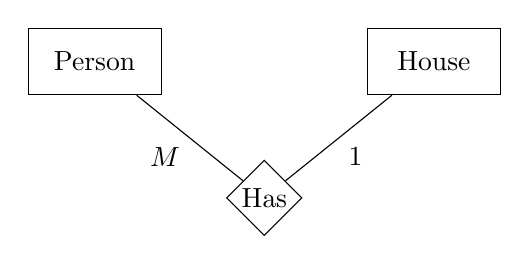
\begin{tikzpicture}[auto,node distance=1.5cm]
            \node[entity] (person) {Person};
            \node[relationship] (has) [below right = of person] {Has} edge node {\(M\)} (person);
            \node[entity] (house) [above right = of has] {House} edge node[midway] {\(1\)} (has);
        \end{tikzpicture}
    \end{center}
\end{highlight}

\subsubsection{Many to Many}\label{ssub:many_to_many}

For many to many, we use \(M\) to \(N\) so that it is clear that the two numbers can be different.
\begin{highlight}{A many to many relationship}
    \begin{center}
        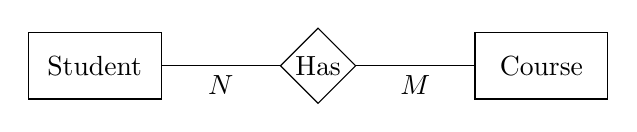
\begin{tikzpicture}[auto,node distance=1.5cm]
            \node[entity] (student) {Student};
            \node[relationship] (enrolls) [right = of student] {Has} edge node {\(N\)} (student);
            \node[entity] (course) [right = of enrolls] {Course} edge node {\(M\)} (enrolls);
        \end{tikzpicture}
    \end{center}
\end{highlight}
Because it can be hard to represent a many to many relationship in a database we can also do something like:

\begin{highlight}{A many to many alternative}
    \begin{center}
        \begin{tikzpicture}[auto,node distance=1.5cm]
            \node[entity] (student) {Student};
            \node[relationship] (has) [below = of person] {Has} edge node {\(1\)} (student);
            \node[entity] (enrollment) [right = of has] {Enrollment} edge node {\(N\)} (has);
            \node[relationship] (in) [right = of enrollment] {In} edge node {\(N\)} (enrollment);
            \node[entity] (course) [above = of in] {Course} edge node {\(1\)} (in);
        \end{tikzpicture}
    \end{center}
\end{highlight}

\subsubsection{Keys}\label{ssub:keys}

The \emph{primary key} is a field (or fields) that uniquely identify each record.
Primary keys must contain unique values and cannot contain null values.
A table can only have one primary key.

A \emph{foreign key} is used to link two tables together.
A foreign key should point to a primary key on another table.

\subsubsection{Compressed Chen Notation}\label{ssub:compressed_chen_notation}

The difference between Chen and Compressed Chen notation is that with regular Chen, the attributes are all around the entities and with Compressed Chen, we just use a table.

\paragraph{Chen}\label{par:chen}

Chen with the combined entities and attributes:

\begin{highlight}{Chen notation}
    \begin{center}
        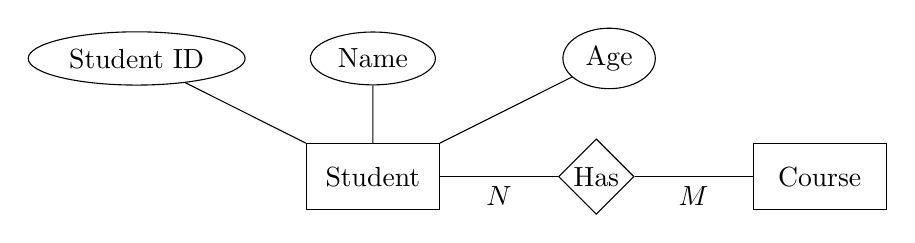
\begin{tikzpicture}[auto,node distance=1.5cm]
            \node[entity] (student) {Student}
            [grow=up,sibling distance=3cm]
            child {node[attribute] {Age}}
            child {node[attribute] {Name}}
            child {node[attribute] {Student ID}};
            \node[relationship] (enrolls) [right = of student] {Has} edge node {\(N\)} (student);
            \node[entity] (course) [right = of enrolls] {Course} edge node {\(M\)} (enrolls);
        \end{tikzpicture}
    \end{center}
\end{highlight}

\paragraph{Compressed Chen}\label{par:compressed_chen}

\begin{highlight}{Compressed Chen with a separate table}
    \begin{minipage}{0.57\linewidth}
        \centering
        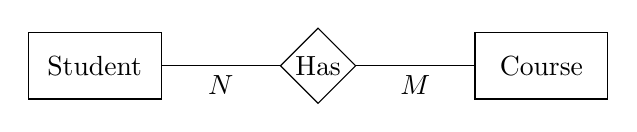
\begin{tikzpicture}[auto,node distance=1.5cm]
            \node[entity] (student) {Student};
            \node[relationship] (enrolls) [right = of student] {Has} edge node {\(N\)} (student);
            \node[entity] (course) [right = of enrolls] {Course} edge node {\(M\)} (enrolls);
        \end{tikzpicture}
    \end{minipage}
    \hfill
    \begin{minipage}{0.40\linewidth}
        \centering
        \begin{tabular}{cc}
            \toprule
            Field      & Type    \\
            \midrule
            Age        & Integer \\
            Name       & String  \\
            Student ID & String  \\
            \bottomrule
        \end{tabular}
    \end{minipage}
\end{highlight}

\subsection{Creating Tables}\label{sub:creating_tables}

To create tables we can use:
\begin{itemize}
    \item SQL \mintinline{sql}{CREATE} statements
    \item phpMyAdmin
\end{itemize}

\subsubsection{Converting to Django Models}\label{ssub:converting_to_django_models}

In Django, instead of creating tables manually, we can just create a few classes.
In Django, every model is automatically assigned an id.
To create relationships, we can just refer to the model instead of the id itself.

\begin{highlight}{Converting tables to Django models}
    \begin{code}{python}
        class House(models.Model):
            pass # Code here

        class Person(models.Model):
            # Every person must live in a house
            house = models.ForeignKey(House)
    \end{code}
\end{highlight}

\section{Presentations}\label{sec:presentations}

A presentation should be given in class on 2021-04-23 for a total of \(5\%\) of your total grade.

Each group will be asked to present the design specification for a web application which you won't have to actually implement.
The presentation should include:
\begin{itemize}
    \item Overview
    \item Personas
    \item A specification
    \item System architecture design
    \item ER diagram
    \item User interface wireframes
    \item A list of technologies to use
\end{itemize}

\section{Client Side Environment}\label{sec:client_side_environment}

We will be focussing on the document object model today (DOM).
We should remember that not all clients are web browsers and may not even be humans.

\subsection{The Beginning of the Web}\label{sub:the_beginning_of_the_web}

Tim Berners Lee was working at CERN where he developed the first web server, browser, HTML and the HTTP protocol all of which ran only on the Next computer system.

\begin{quote}
	``The WorldWideWeb (WWW) project aims to allow links to be make to any information anywhere.''
\end{quote}

\subsection{The Document Object Model (DOM)}\label{sub:the_document_object_model_dom_}

\begin{quote}
	``The Document Object Model is a platform -- and language -- neutral interface that will allow programs and scripts to dynamically access and update the content, structure and style of documents.
	The document can be further processed, and the results of that processing can be incorporated back into the presented page.''
\end{quote}
Everything in the HTML DOM is a node.
The document itself is a document node (usually only has a \mintinline{html}{<html>} child) which contains all of the HTML element nodes with each of their HTML attributes as attribute notes.
The text inside of a HTML element is a text node and comments are in comment nodes (who'd have thought?).

\subsubsection{Element Properties}\label{ssub:element_properties}

Using JavaScript we can get or set the content or attributes of an HTML element.
\begin{description}
	\item[\mintinline{javascript}{el.innerHTML}] Gets the text value of an element.
	\item [\mintinline{javascript}{el.nodeName}] Gets the type of node.
	\item[\mintinline{javascript}{el.nodeValue}] The value stored in a node, this is similar to \mintinline{javascript}{el.innerHTML} but only gets the raw text.
	\item[\mintinline{javascript}{el.parentNode}] Gets the parent node.
	\item[\mintinline{javascript}{el.childNodes}] Get the child nodes.
	\item[\mintinline{javascript}{el.attributes}] Gets attribute nodes.
\end{description}

\subsubsection{Element Methods}\label{ssub:element_methods}

\begin{description}
	\item[\mintinline{javascript}{el.getElementById(id)}] Get an element by its ID, usually this is called on the entire document and not individual elements.
	\item[\mintinline{javascript}{el.getElementsByTagName(name)}] get all elements with a specified tag name.
	\item[\mintinline{javascript}{el.appendChild(node)}] Insert a child node.
	\item[\mintinline{javascript}{el.removeChild(node)}] Removes a child from a node.
\end{description}

\subsubsection{Advantages of the DOM}\label{ssub:advantages_of_the_dom}

\begin{itemize}
	\item The XML/tree structure makes the DOM easy to navigate using attributes, etc.
	\item XML/Structure of the tree is modifiable so the elements, values and structure can be modified, added or changed
	\item It has been standardised by W3C.
\end{itemize}

\subsubsection{Disadvantages of the DOM}\label{ssub:disadvantages_of_the_dom}

\begin{itemize}
	\item Can be resource intensive for very large documents since the whole thing needs to be in memory.
	\item Can be slow since the speed depends on the complexity and size of the tree.
	\item Not the best choice for all usages -- a graphic s intensive application will be not be suited to the model.
	      You should use the canvas directly using OpenGL.
\end{itemize}

\subsubsection{Working with the DOM}\label{ssub:working_with_the_dom}

We can use:
\begin{itemize}
	\item XHTML
	\item CSS
	\item JavaScript
	\item jQuery
	\item AJAX
	\item XML
	\item DOM/SAX parsing
\end{itemize}

\subsubsection{Monitoring User Interactions}\label{ssub:monitoring_user_interactions}

We can detect the user performing an action with our page like clicking, mousing over, double clicking or which keys were pressed.

\paragraph{Event Object}\label{par:event_object}

Each event has an associated object.

\paragraph{Event Handling}\label{par:event_handling}

Like any interactive application, events can be caught and used to execute functions like form validation.

\paragraph{Event Flow}\label{par:event_flow}

Each event object has an ``Event Target'' which is any node in the tree where the event came from.
There are two main types of event flow: event capture (global handling) and event bubbling (local handling).
Every event follows a ``round trip'' model.

\paragraph{Event Capture}\label{par:event_capture}

The event propagates downwards through an element's ancestors.
Any event listeners of the element will be executed.
Ancestors can the potentially handle the event on the way back up again.


\section{Client Side Scripting - JavaScript}\label{sec:client_side_scripting}

\textbf{JavaScript is not Java}.
The name is probably a marketing idea and was originally called \emph{LiveScript} which was created by the folks at \emph{Netscape} for \emph{Navigator}.

JavaScript looks like a procedural language, but it is probably closer to being a functional language since functions are first class objects.
The support of anonymous functions is heavily used by jQuery.

Earlier versions of JavaScript lacked object oriented programming support and excepting handling.
Newer versions (those after Netcape) are handled by ECMA.
ECMA are not very good at writing standards so JavaScript has lots of issues (it's a bit better now).

\subsubsection{Design Errors}\label{ssub:design_errors}

\begin{itemize}
	\item There are very few useful error messages (also helped by there being no compiler since it is interpretted).
	\item Semi-colons are required, but the programmer is not required to put them in since the interpreter just guesses where to put them.
	\item Type coercion is super funky with numbers and strings being coerced to each other with the \mintinline{javascript}{+} operator, for example.
\end{itemize}

\subsubsection{Object Oriented Programming}\label{ssub:object_oriented_programming}

JavaScript has objects with encapsulate data and methods, but all properties are public.
Inheritance is super broken.

\subsubsection{Broken Implementations}\label{ssub:broken_implementations}

Each browser can implement its own engine.
These engines could be extra buggy.
The JavaScript performance was helped make this better though.

\subsubsection{Accessibility}\label{ssub:accessibility}

JavaScript is very easy to write, so lots of amateur programmers can write terrible code.

\subsection{Core Features}\label{sub:core_features}

\begin{itemize}
	\item Interpreted so no compiler is needed.
	\item Some typing (of the dynamic nature) with some basic primitive types.
	\item Syntactically similar to Java or C.
	\item Kind of object oriented.
	\item Has first class anonymous functions.
	\item Scripts can be used inside of HTML which is good for experimentation, but bad for separation of concerns.
\end{itemize}

\subsection{Ways of Including JavaScript}\label{sub:ways_of_including_javascript}

\subsubsection{Embedded}\label{ssub:embedded}

Having all of the code in the \mintinline{html}{<head>} section of the code.
This is bad for the separation of concerns.

\subsubsection{External JavaScript}\label{ssub:external_javascript}

We have an external JavaScript file that is then included like a style sheet in the \mintinline{html}{<head>} section.

\subsection{DOM Integration}\label{sub:dom_integration}

The intent behind JavaScript is to dynamically manipulate documents.
HTML documents are modelled using the DOM.
DOM methods and properties can be modified using JavaScript.

\subsection{Regular Expressions}\label{sub:regular_expressions}

A regular expression is an object that describes a pattern of text that can be matched against and replaced (if needed).
RegExps can be considered a program within a program which is probably why they are quite tricky.

\subsubsection{RegEx in JavaScript}\label{ssub:regex_in_javascript}

In JavaScript, regular expressions are represented as RegExp objects.
\begin{highlight}{JavaScript regular expressions}
	\begin{code}{javascript}
		// Matches "colour" and "color" case-insensitivly
		let pattern = /colou?r/i;
	\end{code}
\end{highlight}
The JavaScript \mintinline{javascript}{search} function can be called on a string with a RegExp as the parameter to search (returns the character index of the match).
The JavaScript \mintinline{javascript}{exec} function can be called on a RegExp object with a string as the parameter returns the matching text, use \mintinline{javascript}{test} to return a boolean.

\section{jQuery}\label{sec:jquery}

JavaScript has very few built in tools (standard library) so we have to write lots of boilerplate code to get anything working.
We should use an extra standard library that focuses on a specific task (user interaction, animation, etc.)
We have:
\begin{itemize}
	\item jQuery
	\item Prototype
	\item Yahoo UI
	\item Moot Tools
\end{itemize}

\subsection{jQuery}\label{sub:jquery}

One of the most popular JavaScript libraries that simplifies client-side scripting.
\begin{itemize}
	\item Selecting DOM elements
	\item Creating UI animations and elements
	\item Handling events
	\item Developing AJAX applications
\end{itemize}

\subsection{Cross Browser Compatibility}\label{sub:cross_browser_compatibility}

Since lots of browsers support different code, we might have to use different JavaScript for different browsers (using browser sniffing).
jQuery fixes this by acting as a layer of abstraction over the browser.

\subsection{Plugins}\label{sub:plugins}

jQuery creases a foundation for additional functionality to be added.
There are lots of added features for images, animations and lots more.

\subsection{Syntax}\label{sub:syntax}

jQuery uses a patterns of selecting and acting on a particular DOM element and altering its parameters.
Selectors can be reused.
\begin{minted}[linenos,numbersep=5pt,frame=lines,framesep=2mm]{javascript}
$('p').css('color', 'blue');
\end{minted}
jQuery uses the pattern, making use of anonymous functions and chaining functions together.
We can use \mintinline{javascript}{(document).ready} to make sure the document is loaded before we to anything to it.
\begin{note}
	Instead of using \mintinline{javascript}{$(document).ready()}, we can use \mintinline{javascript}{$()} as shorthand.
\end{note}

\subsection{Attaching Event Handlers}\label{sub:attaching_event_handlers}

\begin{minted}[linenos,numbersep=5pt,frame=lines,framesep=2mm]{javascript}
$(document).ready(function() {
  $("#button").click(function() {
    $("#message").css("color", "blue");
    if ($("#message").is(":visible")) {
      $("#message").hide();
    } else {
      $("#message").show();   
    }
  })
})
\end{minted}


\section{Web Application Frameworks}\label{sec:web_application_frameworks}

\subsection{Why use a framework?}\label{sub:why_use_a_framework_}

Once you have developed several web applications, it will be very clear that you are repeatedly implementing the same few pieces of functionality.
Using a framework will give you well tested and robust implementations for database handling, templating, and for having good separation of concerns.

\subsubsection{Pre-fabricated Wheels}\label{ssub:pre_fabricated_wheels}

A web application framework will usually provide pre-built classes for:
\begin{itemize}
    \item Authentication
    \item Database abstraction (or ORM)
    \item Template system
    \item An AJAX sub-framework
    \item Session management
    \item An architecture based on the model-view-controller system
\end{itemize}

\subsection{Model View Controller}\label{sub:model_view_controller}

The MVC pattern separates data and business logic from presentation.
In web applications:
\begin{itemize}
    \item The view is often HTML generated by the application
    \item The controller receives GET or POST requests and processes data.
    \item The model then gets the data needed to carry out the task.
\end{itemize}

\subsubsection{What is a design pattern?}\label{ssub:what_is_a_design_pattern_}

A design pattern is a tool to communicate ideas, solutions and knowledge about a common design problem which can be expressed hierarchically as a three part rule between a context, a problem, and a solution where each stage in the hierarchy has its own level of granularity.
A software design pattern can be paired with a user interface design pattern to help developers create effective and usable user interfaces.

\begin{note}
    Although there are standard ways to implement a design pattern, there can be more than one for each pattern; it is up to the developer to choose which to use.
\end{note}

\subsubsection{MVS and GUIs}\label{ssub:mvs_and_guis}

The MVC design pattern was originally invented in the \(1970\)s by Xerox where it was used to map mouse and keyboard inputs to actions.
The actions Xerox used were sent to either the model -- or the application state, or database -- or update the display.

\begin{description}
    \item[Controller] Interprets user input
    \item[Model] Handles data for the application
    \item[View] Manages and represents data
\end{description}

\subsubsection{Model}\label{ssub:model}

Contains code that operates on the application data.
All CRUD operations must go through this layer:
\begin{itemize}
    \item Retrieve or query the state
    \item Create new data
    \item Update the current state
    \item Delete
\end{itemize}
A model is a class which represents the application data and domain logic.
When data in the model is changed, it will trigger an update on the views, but views can query the model at any time.
A controller can also access the model, where some of the application data functionality will be kept.

\subsubsection{View}\label{ssub:view}

The view is a visual representation of a model that defines how the pages should look and how the user can submit actions to be executed with the controller.
A view is attached to a model so when the model changes, the view must update too using one of two methods:
\begin{description}
    \item[Push model] View registers itself with the model for change notifications
    \item[Pull model] the view calls the model when it needs the most up to date data.
\end{description}
The view is responsible for forwarding user requests to the controller.

\subsubsection{Controller}\label{ssub:controller}

The controller defines the application behaviour by controlling the flow of the program by receiving and processing user commands on the model which get output to the view -- which links the user to the application system.

By separating the model from the controllers and views, we can show different data or layouts to many different people for many different people.

\subsubsection{MVC advantages}\label{ssub:mvc_advantages}

\begin{itemize}
    \item Enable independent development and testing (model, view, controllers can be different teams)
    \item Easier to maintain
    \item Provides reusable view s and model
    \item Sync views and multiple simultaneous views
    \item Enforce logical separation of concerns
\end{itemize}

\subsubsection{Disadvantages}\label{ssub:disadvantages}

\begin{itemize}
    \item More initial overhead (\(3\) classes vs \(1\)) especially for simple applications
    \item Debugging can be a problem (is it a model problem, view problem, etc.)
    \item Required the developers to understand patterns.
\end{itemize}

\section{Frameworks}\label{sec:frameworks}

As with frameworks in the real world (eg.\ a building frame or vehicle chassis), software frameworks have designs and partial implementations for a specific domain of applications.
Frameworks allow developers to create applications faster by giving sane default functionality to be extended and overridden.

\subsection{Framework definitions}\label{sub:framework_definitions}

\begin{itemize}
    \item A set of abstract classes for a family of problems.
    \item A frameworks is the reusable design of a system of abstract classes and how those interact.
    \item A framework is a reusable software architecture made of both design and code.
\end{itemize}

\subsection{The Characteristics of a Framework}\label{sub:characteristics}

\begin{itemize}
    \item Inversion of control: framework is responsible for the application control flow.
    \item Sane and useful default behaviour is provided
    \item Extensibility means plugins can be used for specific purposes
    \item Non-modifiable framework code where key components cannot be altered.
\end{itemize}

\subsection{Why should you use a framework?}\label{sub:why_frameworks}

\begin{itemize}
    \item All applications have common requirements: security, password recovery, database management, session management which a framework can include and provide high levels of support for.
    \item Frameworks encapsulate the thousands of hours of experience from each of the authors that is improved on each iteration.
    \item They can often support very large amounts of traffic right out of the box.
    \item Allows for a rapid development for rapid release cycle that is common with web development.
    \item Reduce the development effort of programming in several programming languages (HTML, CSS, SQL, Javascript).
    \item Manage the complexity of large web applications like user authentication, session management, etc.
    \item Reduce boilerplate code (CRUD, session management).
    \item A framework allows you to focus only on what makes the application unique.
    \item Increased security (until an exploit is found in the framework and your application is now vulnerable).
    \item Frameworks are extensively tested so are very robust.
\end{itemize}

\subsection{Why should you not use a framework?}\label{sub:why_should_you_not_use_a_framework_}

\begin{itemize}
    \item Inversion of control gives away some of the control a developer usually has
    \item Code outside of what is supported can be \emph{very} difficult
    \item Frameworks can introduce extra code bloat
    \item Levels of abstraction can introduce performance penalties
    \item Frameworks can have a very steep learning curve
    \item Can be poorly documented
    \item A bug or security problem can seriously compromise the application
\end{itemize}

\subsection{Frameworks vs Libraries}\label{sub:frameworks_vs_libraries}

Framework is about reusing behaviours by controlling how abstract classes and components interact with each other.
A framework will call your own application code, whereas a library just adds additional reusable functionality to your existing application.



\part{Semester Three (2021-11-01)}
\chapter{Practical Algorithms}\label{cha:practical_algorithms}

\etocsettocstyle{\section*{\contentsname}\par}{}
\etocsetnexttocdepth{subsubsection}
\localtableofcontents

\section{Course Introduction}\label{sec:course_introduction}

The course will be worth 20 credits, so will be slightly easier than last semester's CANS.

We will spend the course talking about what algorithms are.
Simply an algorithm is a  step by step method for completing a task.
If we are able to specify an algorithm for a problem, we are able to automate its solution.

In general, the field of computing science is the study of mathematical, linguistic, and hardware representations of algorithms.
\begin{description}
    \item[Mathematical] We need to make sure algorithms are efficient and correct.
    \item[Hardware] We need to make machines to complete the algorithms.
    \item[Linguistic] We need to make programming languages to express algorithms in.
\end{description}

\subsection{Learning Outcomes}\label{sub:learning_outcomes}

\begin{enumerate}
    \item We will implement basic data structures
    \item We will learn to use recursion
    \item We will analyse and implement algorithms
    \item We will use mathematics to write and prove assertions about our algorithms
    \item Understand inductively generated structures and proofs
    \item Use basic combinatorics to solve mathematical problems
\end{enumerate}

In general we will be focusing on problem-based learning to complete these objectives.

\subsection{Class Times}\label{sub:class_times}

Class time will be split \(60\%\) to \(40\%\) where \(40\%\) of the time will be spent with ``online any time'' lectures, and the remaining ``60\%'' will be live workshops that will require a pen, paper, and at least one laptop.

\subsection{Assessments}\label{sub:pa_assessments}

\begin{description}
    \item[Workshop Participation] Worth \(10\%\) which is either awarded or isn't awarded.
    \item[Class Tests] There will be a total of 5, where each one is worth \(1\%\) of the total course.
    \item[First Coursework Task] This will be a programming task worth \(15\%\) of the entire course and will be due on \(2021-12-16\).
    \item[Second Coursework Task] This will be a written exercise worth \(10\%\) that is dues on \(2022-01-09\).
    \item[Final Exam] There will be a problem-based final exam on \(2022-02-09\) that will be worth the remaining \(60\%\) of the course.
\end{description}

\subsection{Applications of Algorithms}\label{sub:applications_of_algorithms}

\begin{enumerate}
    \item Game Design
    \item Film special effects
    \item Most areas of mathematics and physics
    \item Computer simulations
    \item Finding organ transplants
    \item Artificial Intelligence
    \item Natural language processing
\end{enumerate}

\section{Writing Programs to Solve Problems}\label{sec:writing_programs_to_solve_problems}

There are three phases to any algorithmic computer program:
\begin{enumerate}
    \item Input
    \item Process
    \item Output
\end{enumerate}
Data processing is the step we are most interested in.
Here we need to think computationally by avoiding intuitions, guesses and feelings that aren't available to a computer.

\subsection{Thinking Like a Computer}\label{sub:thinking_like_a_computer}

\begin{description}
    \item[Algorithmic Thinking] We need to create a logical flow of thinking for the computer to follow.
    \item[Analysis] We need to create accurate, fast solutions to our problems.
    \item[Decomposition] Problems need to be broken down.
\end{description}
Along with these more algorithmic styles of thinking, we also need to be able to \emph{abstract} and \emph{generalise} problems.

In an algorithmic program, we have access to three types of operations: \emph{sequential}, \emph{conditional}, iterative -- which are all quite self explanatory.

\subsubsection{Sequential}\label{ssub:sequential}

A sequential operation is one which performs a process.
The program flow goes straight in one side and right out the other.

\subsubsection{Conditional Operations}\label{ssub:conditional_operations}

A conditional operation asks a question, then performs an operation based on the results.

\section{Writing Algorithms}\label{sec:writing_algorithms}

Some algorithms -- eg. binary search here -- don't have a linear increase in their time complexity for a linear increase to the number of elements.
For a binary search we have a \(\log(n)\) graph instead.

We don't just have to worry about time complexity though, we also have memory (storage) complexity to worry about too.

\begin{highlight}{A logarithmic graph}
    For a \(\log\) graph, the \(y\) value increases very quickly at first, before levelling off.
    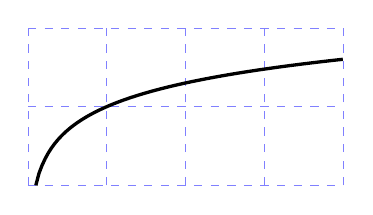
\begin{tikzpicture}
        \draw [help lines] (0, 0) grid [step=1] (4,2);
        \draw[domain=0.1:4,samples=100, very thick] plot (\x,{1 + log10(\x)});
    \end{tikzpicture}
\end{highlight}

We we need to search through unsorted data, maybe it's easier to sort the data first then store the sorted results for various searching operations later.

For sorting algorithms, there are two types of algorithm: \emph{in-place} and \emph{out-of-place} where an in-place sort doesn't create a new array, but an out-of-place one does, and therefore uses less memory.

\subsection{Planning}\label{sub:planning}

We should always plan an algorithm before we start to write it, where we clearly illustrate the final goal and all required intermediary steps.

\subsubsection{Pseudo code}\label{ssub:pseudocode}

There is no standard way of writing pseudo code, but in general instructions like \mintinline{text}{INPUT}, \mintinline{text}{OUTPUT}, \mintinline{text}{WHILE}, \mintinline{text}{FOR} and \mintinline{text}{IF} are used.

\subsubsection{Flow Charts}\label{ssub:flow_charts}

Flow charts are similar in that there is no standard way to represent them either.
A flow chart is different in that it shows the instructions as a diagram instead of a list of operations.


\section{Data Structures}\label{sec:data_structures}

We almost always want to work with collections of data, so we almost always must use a \emph{data structure}.

For data to work in a data structure, there must be some relationship between all of the pieces of data.
The standard data structures are:
\begin{itemize}
    \item Arrays
    \item 2D arrays
    \item Records/dictionaries
    \item Stacks
    \item Queues
\end{itemize}

\section{Algorithmic Analysis}\label{sec:algorithmic_analysis}

When we write an algorithm, there are several characteristics we want it to have:
\begin{itemize}
    \item Correct
    \item Readable
    \item Reusable
    \item Testable
    \item Elegant
    \item Efficient (in terms of time and space)
\end{itemize}

\subsection{Time Efficiency}\label{sub:time_efficiency}

For estimating the time efficiency of an algorithm, we can use the following equation to make an approximation.
\[
    \mathrm{Execution Time} \approx \mathrm{Number of steps}
\]
We are able to use this because it's not very useful to get a time value for one particular value of \(n\), and this makes it easier to look at the overall trend of the time efficiency as \(n\) changes.
We can do this experimentally, but that isn't great since it's slow and depends on specific implementation details (like language, or system specifications) to create a representation of an algorithm.
\begin{quote}
    ``Algorithms analysis is a way to compare the time and space efficiency of algorithms with respect to possible inputs, but irrespective of other context.''
\end{quote}
When we are calculating the time efficiency theoretically, we should use a high level description of an algorithm, instead of a specific implementation, to create a function in terms of \(n\), ie.\ \(T(n)\).

\begin{highlight}{A comparison of the empirical and theoretical approaches to calculating time complexity}
    \begin{tabular}{p{6cm}p{6cm}}
        Empirical                                   & Theoretical                                 \\
        \midrule
        Can be difficult to implement the algorithm & No need to write an implementation          \\
        \midrule
        Results may be input dependant              & We can calculate the run time for all \(n\) \\
        \midrule
        The same hard/soft ware must always be used & Considers all possible inputs               \\
        \midrule
        Results may be more realistic in context    & Independent of hard/software                \\
        \midrule
                                                    & Results are only indicative                 \\
    \end{tabular}
\end{highlight}

\subsection{Best, Worst, and Average Case}\label{sub:best_worst_and_average_case}

The \emph{best case} is generally useful to know, but not really practical since it often ends up \(1\) or \(n\).
The \emph{average case} is sometimes useful for creating an estimate.
The \emph{worst case} is most useful because it is a guarantee that a particular algorithm will never take more than this time.

\section{Big O Complexity}\label{sec:big_o_complexity}

For calculating the \emph{big O complexity}, we want tot approximate the number of steps a particular algorithm uses to solve a particular problem in terms of \(n\) to create a function like \(f(n)\).
This means that big O is \(O(f(n))\).

\subsection{Typical Complexities}\label{sub:typical_complexities}

\subsubsection{\(O(1)\)}\label{ssub:mkoone}

The time complexity here is always constant regardless of the value of \(n\), therefore this is the very best big O complexity.
\begin{highlight}{Graph of \(O(1)\)}
    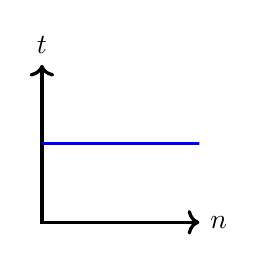
\begin{tikzpicture}
        \draw[very thick, <->] (2, 0) node[right] {\(n\)} -| (0, 2) node[above] {\(t\)};
        \clip (0,0) rectangle (2,2);
        \draw[very thick, scale=1, domain=0:2, smooth, variable=\t, blue] plot ({\t}, {1});
    \end{tikzpicture}
\end{highlight}

\subsubsection{\(O(n)\)}\label{ssub:mkon}

A \(O(n)\) time complexity is a linear growth, that can be imagined as handing out sweets to your friends.
By doubling \(n\), we double \(t\), so this is generally considered a ``good'' growth.
\begin{highlight}{Graph of \(O(n)\)}
    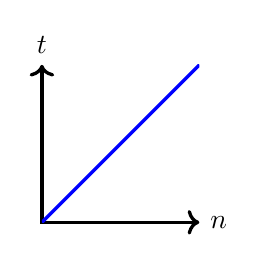
\begin{tikzpicture}
        \draw[very thick, <->] (2, 0) node[right] {\(n\)} -| (0, 2) node[above] {\(t\)};
        \clip (0,0) rectangle (2,2);
        \draw[very thick, scale=1, domain=0:2, smooth, variable=\t, blue] plot ({\t}, {\t});
    \end{tikzpicture}
\end{highlight}

\subsubsection{\(O(n^2)\)}\label{ssub:mkonsr}

This can be imagined as everyone giving everyone else a hug at a party, so for \(n\) guest, \(t\) will be \(\frac{n^2+n}{2}\).
The dominant term here is the \(n^2\), so the time complexity of the algorithm is \(O(n^2)\).

\begin{highlight}{Graph of \(O(n^2)\)}
    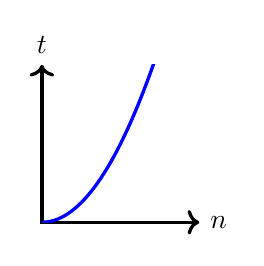
\begin{tikzpicture}
        \draw[very thick, <->] (2, 0) node[right] {\(n\)} -| (0, 2) node[above] {\(t\)};
        \clip (0,0) rectangle (2,2);
        \draw[very thick, scale=1, domain=0:2, smooth, variable=\t, blue] plot ({\t}, {\t*\t});
    \end{tikzpicture}
\end{highlight}

\subsubsection{\(O(2^{n})\)}\label{ssub:mkontwotdn}

Here we have an \emph{exponential growth}, so if \(n\) increases by \(1\), then \(t\) will double.
This is a pretty bad growth.

\begin{highlight}{Graph of \(O(2^n)\)}
    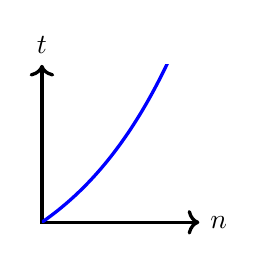
\begin{tikzpicture}
        \draw[very thick, <->] (2, 0) node[right] {\(n\)} -| (0, 2) node[above] {\(t\)};
        \clip (0,0) rectangle (2,2);
        \draw[very thick, scale=1, domain=0:2, smooth, variable=\t, blue] plot ({\t}, {2^(\t)-1});
    \end{tikzpicture}
\end{highlight}

\subsubsection{\(O(\log n)\)}\label{ssub:mkologn}

This is the inverse of the exponential function, so you have to double \(n\) to increase \(t\) by \(1\), because every step halves the remaining size.
This is a \emph{very} good time complexity.

\begin{highlight}{Graph of \(O(\log n)\)}
    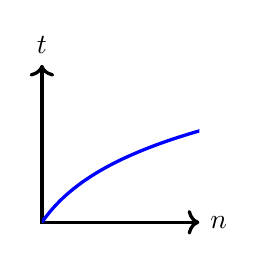
\begin{tikzpicture}
        \draw[very thick, <->] (2, 0) node[right] {\(n\)} -| (0, 2) node[above] {\(t\)};
        \clip (0,0) rectangle (2,2);
        \draw[very thick, scale=0.5, domain=0.01:6, smooth, variable=\t, blue] plot ({\t-1}, {log2(\t)});
    \end{tikzpicture}
\end{highlight}

\subsubsection{\(O(n!)\)}\label{ssub:mknfac}

A \emph{factorial} growth is \emph{very} bad because it grows \emph{very} fast.

\begin{highlight}{Graph of \(O(n!)\)}
    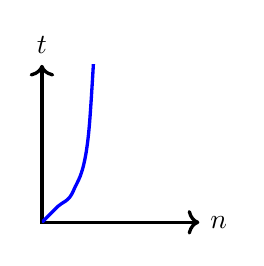
\begin{tikzpicture}
        \draw[<->, very thick] (2, 0) node[right] {\(n\)} -| (0, 2) node[above] {\(t\)};
        \clip (0,0) rectangle (2,2);
        \draw[very thick, smooth, blue] plot [smooth] coordinates{ (0, 0) (0.2, 0.2) (0.4, 0.4) (0.6, 1.2) (0.8, 4.8)};
    \end{tikzpicture}
\end{highlight}

\subsubsection{Others}\label{ssub:others}

We also have:
\begin{itemize}
    \item \(O(\sqrt{n}\) or \(O(n^{\frac{1}{2}})\) which is better than \(O(n)\), but worse than \(O(\log n)\).
    \item \(O(n \log n)\) which is sometimes called ``quasilinear'' and usually comes from having a \(O(\log n)\) operation in a \(O(n)\) loop.
\end{itemize}

\subsubsection{In Order of Goodness}\label{ssub:in_order_of_goodness}

\begin{enumerate}
    \item \(O(1)\)
    \item \(O(\log n)\)
    \item \(O(\sqrt{n})\)
    \item \(O(n)\)
    \item \(O(n \log n)\)
    \item \(O(n^2)\)
    \item \(O(n^3)\)
    \item \(O(2^{n}\)
    \item \(O(n!)\)
\end{enumerate}

\subsection{Finding The Big O Complexity}\label{sub:finding_the_big_o_complexity}

\begin{enumerate}
    \item Count the primitive operations (things like assignments, array index lookups, method calls, and returning). You should take an input \(n\), then output a function \(f(n)\). Note: remember to count operations in arrays properly.
    \item Express the number of steps as a function of \(n\) like \(T(n)=7n + 2\).
    \item Find the dominant part of the equation. We are looking at the growth rate of the function, so we can ignore all terms except the highest order one.
\end{enumerate}

\subsection{Rules for finding big O complexities}\label{sub:rules_for_finding_big_o_complexities}

\begin{enumerate}
    \item \textbf{Loops}: count the number of primitive operations as \(\mathrm{operations in loop} * \mathrm{total iterations}\)
    \item \textbf{Nested Loops}: we should analyse from the inside loop through to the outside loop, multiplying by the number of iterations each time.
    \item \textbf{Consecutive Operations}: simply add the operations
    \item \textbf{If-then-else}: have one operation for the conditional check, then assume the worst case
    \item \textbf{Constants}: remove the constant multiplier because it doesn't affect the final graph's shape
    \item Drop all lower order terms
    \item Always assume the worse case scenario
\end{enumerate}

\subsection{Big Omega}\label{sub:big_omega}

Big Omega (\(\Omega\) represents the best case scenario (ie.\ the fastest possible speed that an algorithm can perform at).
Big omega and big O can be used to calculate the enclosing bounds of the algorithm's performance.

\section{Bubble Sort}\label{sec:bubble_sort}

\begin{enumerate}
    \item Compare \(i\) with \(i+1\), swap if bigger.
    \item Repeat until the end of the array.
    \item Move the ``last index'' one position closer the start of the array so that we don't re-sort already sorted elements.
\end{enumerate}


\section{Mathematical Sets}\label{sec:mathematical_sets}

Sets are a (the?) fundamental component to all mathematics.
Even the concept of functions is built upon the idea of sets, since a function just assigns the numbers from one set on to another set.

\subsection{Definition}\label{sub:definition}

A \emph{set} is a collection of objects (named \emph{members}) where the most important aspect of the set is the membership, therefore we can consider a set to be unordered.
\begin{itemize}
    \item We only care about membership, so the order or being able to sort it is irrelevant and useless.
    \item We can have duplicates, but they are useless and irrelevant too since we still only care about whether one member is or isn't in the set.
\end{itemize}
\begin{note}
    A set ``contains'' its elements.
\end{note}

\subsubsection{Symbols}\label{ssub:symbols}

To say that \(a\) is a member of \(A\), we say: \(a \in A\). Where we want to say that \(a\) is not a member of \(A\), we say: \(a \notin A\).

\subsection{Notations}\label{sub:notations_pafour}

There are several different ways of representing a set which are all useful on different occasions.

\subsubsection{Roster Method}\label{ssub:roster_method}

We include all of the elements between braces.
\[
    S = \{A, B, C, D\}
\]
We can also use ellipses (\(\dots\)) to show a continuation, but we must make sure that the patterns is unambiguous.
\[
    S = \{1, 2, 3, \dots, 99, 100\}
\]
\begin{note}
    The order and duplicicity here is still irrelevant.
\end{note}
Even though this is the clearest method, there are some limitations:
\begin{itemize}
    \item It is impossible or inconvenient to describe sets which do not follow a very set and clear pattern (like the rational numbers for example).
\end{itemize}

\subsubsection{Set Builder Notation}\label{ssub:set_builder_notation}

Here write an expression that can be expanded to a set.
\begin{align*}
    S & = \{x \mid x \text{ is a positive integer } < 100\}     \\
    O & = \{x \mid x \text{ is a positive odd integer } < 100\} \\
    P & = \{x \in \Z \mid x \text{ is odd and } < 100\}
\end{align*}
Sometimes it is not very easy to write an expression to describe a set, so we can use a predicate function instead.
\[
    S=\{x \mid \mathrm{Prime}(x)\}
\]

\subsection{Common Sets}\label{sub:common_sets}

As well as the sets we define ourselves, there are several sets which are always available and always defined the same.

\begin{description}
    \item[Natural/Counting] \(\N = \{0, 1, 2, 3, 4, \dots\}\)
    \item[Integers] \(\Z = \{\dots, -3, -2, -1, 0, 1, 2, 3, \dots\}\)
    \item[Positive Integers] \(\Z^{+} = \{1, 2, 3, \dots\}\)
    \item[Rational] \(\Q=\{\frac{p}{q} \mid p, q \in \Z, \text{and} \neq 0\}\)
    \item[Real] There is no specific definition, these are just all numbers.
\end{description}

\subsubsection{Universal Set}\label{ssub:universal_set}

The universal set contains all possible elements that are currently under considerations.

\subsubsection{Empty Set}\label{ssub:empty_set}

The empty set is pretty self explanatory -- it simply contains no elements.

\section{Set Equality and Subsets}\label{sec:set_equality_and_subsets}

For this section, we have to first define a few symbols:

\begin{tabular}{ll}
    \toprule
    Symbol           & Description                                                                                                              \\
    \midrule
    \(\forall \)     & For all members                                                                                                          \\
    \(A \implies B\) & If \(A\) is \mintinline{text}{true}, then \(B\) is too.                                                                  \\
    \(A \iff B\)     & If and only if \(A\) is \mintinline{text}{true}, \(B\) is true. \(B\) cannot be \mintinline{text}{true} unless \(A\) is. \\
    \(A \lor B\)     & Logical OR. Used to OR two conditions together.                                                                          \\
    \(A \land B\)    & Logical AND. Used to AND two conditions together.                                                                        \\
    \bottomrule
\end{tabular}

\subsection{Set Equality}\label{sub:set_equality}

Two sets are said to be equal if and only if they have the same elements.
\[
    \forall x(x \in A \iff x \in B) \quad \mathrm{\textbf{OR}} \quad A = B
\]
For all values of \(x\), if \(x\) belongs to \(A\), it also belongs to \(B\).

\subsection{Subsets}\label{sub:subsets}

It can be said that \(A\) is a subset of \(B\) if and only if all of the values in \(A\) are also in \(B\).
\[
    A \subseteq B
\]
Which can be expanded to the more verbose:
\[
    \forall x (x \in A \implies x \in B)
\]
Equal sets are also considered subsets of each other:
\[
    A=B \iff A \subseteq B \land B \subseteq A
\]
\begin{note}
    Since \(\emptyset\) is a subset of all other sets, \(\forall S(\emptyset \subseteq S)\).
    It should also be obvious that every set is a subset with itself: \(\forall S ( S \subseteq S )\)
\end{note}

\subsubsection{Proper Set}\label{ssub:proper_set}

If \(A\) is a subset of \(B\), but \(A \neq B\), then \(A\) is a ``proper subset'' of \(B\).

\section{Set Operations}\label{sec:set_operations}

Set theory is very similar to the boolean algebra covered in CANS, so we will reuse most of the same operations here.

\subsection{Union}\label{sub:unionpafour}

The union of sets \(A\) and \(B\) can be written as:
\[
    A \cup B
\]
which is basically just \(A + B\), but can be written more verbosely like:
\[
    A \cup B = \{x \mid x \in A \lor x \in B\}
\]

\subsection{Intersection}\label{sub:intersection}

The intersection operator selects members which are in \(A\) and \(B\) and can be written as:
\[
    A \cap B = \{x \mid x \in A \land x \in B\}
\]
If \(A \cap B= \emptyset\), then it can be said that \(A\) and \(B\) are disjoint sets.

\subsection{Compliment}\label{sub:compliment}

This is simply everything that is not included in a specific set and is written as:
\[
    \overline{A}=\{x \in \mathbb{U} \mid x \notin A\}
\]
This can be simplified to a much nicer:
\[
    \mathbb{U}-A
\]

\subsection{Difference}\label{sub:differencepafour}

The difference between two sets is all of the elements in \(A\), but not in \(B\) and can be written as:
\[
    A-B = \{x \mid x \in A \land x \notin B\} = A \cap \overline{B}
\]
It's worth mentioning that \(A \cap \overline{B}\) works since \(\overline{B}\) is everything that is not in \(B\), so we can get the intersection of that with \(A\) to get members in \(A\), but not in \(B\).

\section{Set Identities}\label{sec:set_identities}

Similar to boolean algebra, we have several identities which are good to understand.

\subsubsection{Identity Laws}\label{ssub:identity_laws}

\[
    A \cup \emptyset = A \quad A \cap \mathbb{U} = A
\]

\subsubsection{Domination Laws}\label{ssub:domination_laws}

\[
    A \cup \mathbb{U} = \mathbb{U} \quad A \cap \emptyset = \emptyset
\]

\subsubsection{Idempotent Laws}\label{ssub:idempotent_laws}

\[
    A \cup A = A \quad A \cap A = A
\]

\subsubsection{Complementation Laws}\label{ssub:complementation_laws}

\[
    \overline{(\overline{A})} = A
\]

\subsubsection{Commutative Laws}\label{ssub:commutativepafour}

\[
    A \cup B = B \cup A \quad A \cap B = B\cap A
\]

\subsubsection{Associative Laws}\label{ssub:associateivepafour}

\[
    A \cap (B \cap C) = (A \cap B) \cap C \quad A \cap (B \cap C) = (A \cap B) \cap C
\]

\subsubsection{Distributive Laws}\label{ssub:distributive_laws}

\[
    A \cap (B \cup C) = (A \cap B) \cup (A \cap B)
\]
\begin{note}
    This is just like breaking brackets in mathematics. Also to note, we can't move the position of the brackets since there are different operations going on.
\end{note}

\subsubsection{De Morgan's Laws}\label{ssub:de_morgan_s_laws}

\[
    \overline{(A \cup B)} = \overline{A} \cap \overline{B}
\]

\subsubsection{Absorption Laws}\label{ssub:absorption_laws}

\[
    A \cup (A \cap B) = A \quad A \cap (A \cup B) = A
\]

\subsubsection{Complement Laws}\label{ssub:complement_laws}

\[
    A \cup \overline{A} = \mathbb{U} \quad A \cap \overline{A} = 0
\]

\subsubsection{Converting Complements to Difference}\label{ssub:converting_complements_to_difference}

\[
    A \cap \overline{B} = A - B
\]


\section{Static vs Dynamic Data Structures}\label{sec:static_vs_dynamic_data_structures}

\subsection{What is a data structure?}\label{sub:what_is_a_data_structure_}

A collection of data where there is some relationship between the data pieces that we can perform operations on.

\subsection{Static Data Structures}\label{sub:static_data_structures}

Static data structures need to have a maximum size defined when they are first defined.

\subsection{Dynamic Data Structures}\label{sub:dynamic_data_structures}

Dynamic data structures can vary in size at runtime so you can grow the structure as needed.

\subsection{Comparison of Dynamic and Static Data Structures}\label{sub:comparison_of_dynamic_and_static_data_structures}

\begin{tabular}{p{7cm}p{7cm}}
    \toprule
    Dynamic                                                          & Static                                                            \\
    \midrule
    Only use as much memory as needed                                & Memory is fixed, so there is no risk of running out               \\
    Easier to add/remove data                                        & No need to check data size at runtime (you already know the size) \\
    We don't need to know the size in advance                        & Random access is easier                                           \\
    Run the risk of ``overflowing'' if you run out of memory         & Can waste some memory if the whole structure is not used          \\
    Harder to program (you need to keep track of the data structure) & Adding/removing items is slow (part of array needs rewritten)     \\
    Data can be left ``orphaned'' filling up memory with garbage     & Array size must be estimated before use                           \\
    \bottomrule
\end{tabular}

\section{Singly Linked Lists}\label{sec:singly_linked_lists}

This is a sequence of nodes arranged in linear order.
Every node has a \mintinline{text}{key} and a pointer to the next node \mintinline{text}{next}.
For a node \mintinline{text}{x}, the next element will be \mintinline{text}{x.next}.
Where \mintinline{text}{x.next = NIL}, then there is no next element.

\subsection{Head Pointer}\label{sub:head_pointer}

We need a head pointer to point to the first element of the list, so we call that \mintinline{text}{x.head}.
If \mintinline{text}{x.head = NIL}, the list is empty.

\subsection{Insertion}\label{sub:insertiontolinkedlist}

\begin{enumerate}
    \item Start while loop with the condition set to check if the \mintinline{text}{current.next = NILL} to insert at the tail, or \mintinline{text}{current.key = target} to insert after a particular node.
    \item Update \mintinline{text}{current} to \mintinline{text}{current.next} .
    \item Allocate a new node
    \item Update \mintinline{text}{new.next} to point to \mintinline{text}{current.next}
    \item Update \mintinline{text}{current.next} to point to the new node
\end{enumerate}
\begin{note}
    The order here is important since we will ``lose'' the next element if we don't do them in the correct order.
\end{note}
\begin{note}
    Insertion at the tail is useful to implement a first-in-first-out data structure like a queue.
\end{note}
\begin{note}
    If we are already at the head of the list, then we can give a special case to insert at the head with no iteration.
\end{note}

\subsubsection{Time Complexity}\label{ssub:linkedlistinsertcomplexity}

The time complexity of inserting at the head is only \(O(1)\), since we already know where the first element is.
The time complexity of inserting at any other point is \(O(n)\), since we have to loop through the while list.

\subsection{Deletion}\label{sub:linkedlistdeletion}

\begin{enumerate}
    \item Update \mintinline{text}{prev.next} to \mintinline{text}{deleted.next}
    \item Deallocate \mintinline{text}{deleted}.
\end{enumerate}
\begin{note}
    We always have to check that \mintinline{text}{prev.next} is not \mintinline{text}{NIL} so that we know the deleted element exists.
\end{note}

\subsubsection{Time Complexity}\label{ssub:linkedlistdeletecomplexity}

The time complexity of deleting at the head is only \(O(1)\), since we already know where the first element is.

\subsection{Search}\label{sub:linkedlistsearch}

\begin{enumerate}
    \item Starting from \mintinline{text}{current}.
    \item Start while loop with the condition set to check if the \mintinline{text}{current.key = target} -- for example, something like \mintinline{text}{while current.key != target and current != NILL}.
    \item Update \mintinline{text}{current} to \mintinline{text}{current.next}.
    \item Return \mintinline{text}{current} which will either be a pointer to the correct element or \mintinline{text}{NIL} if the search result doesn't exist.
\end{enumerate}

\subsubsection{Time Complexity}\label{ssub:time_complexitysearchlinkedlist}

Because we might need to search through every element of the linked list, the complexity is \(O(n)\).

\subsection{Reducing the time complexity of tail operations}\label{sub:reducing_the_time_complexity_of_tail_operations}

We can add another pointer to the tail end of a linked list, which will allow us to insert or delete directly at the very end of the list without having to traverse all the way through it first.
This does have the downside of requiring inserting and deleting functions to update this new tail pointer.
\begin{note}
    The space complexity is slightly worse here because we're storing another variable, but we do manage to reduce the time complexity of a tail insertion or deletion to \(O(n)\)
\end{note}
\begin{note}
    If the list is empty, we can just perform a regular head insertion for a \(O(1)\) time complexity still.
\end{note}
When we want to delete a node, we need to be able to update the previous node \mintinline{text}{prev}, which can only be done if we traverse the list in order, which we don't do if we jump straight to the end.
This means that deletion of an element of a linked list is always \(O(n)\) unfortunately, unless we can traverse the list in the other direction.

\section{Doubly Linked Lists}\label{sec:doubly_linked_lists}

A doubly linked list is very similar to a regular linked list, except it has a \mintinline{text}{node.prev} pointer in addition to the existing \mintinline{text}{node.next} pointer, that points to the (you guessed it!) previous node.
This has the downside that there is a larger memory overhead to the list, but some operations are much more efficient and simple.
\begin{note}
    As with \mintinline{text}{node.next}, if \mintinline{text}{node.prev} is \mintinline{text}{NIL}, then we are at the head of the linked list.
\end{note}

\subsection{Deletion}\label{sub:deletionofelementsonadoublylinkedlist}

To perform a deletion, we need to update the next and previous nodes in the list.
We don't need to worry about

\begin{enumerate}
    \item Update \mintinline{text}{prev.next} to \mintinline{text}{delete.next}, if the previous node is \mintinline{text}{NIL}, we need to update the head instead.
    \item Update \mintinline{text}{next.prev} to \mintinline{text}{delete.prev}, if the next node is \mintinline{text}{NIL}, we don't need to do anything since \mintinline{text}{NIL} has no \mintinline{text}{prev} value.
\end{enumerate}


\section{Mathematical Functions}\label{sec:mathematical_functions}

It is very important to note that we are not talking about programming functions, here we are specifically talking about mathematical functions which maps one input value directly to exactly one output value (we use the work ``unambiguous'').
However, one output can come from more than one input (\(f(x) = x^2\)) for example will have this.

A function \(f\) from set \(A\) to set \(B\) is illustrated as \(f: A \iff B\), which can be said as: ``assign each element from \(A\) to exactly one element from \(B\).
\begin{note}
    Sometimes functions are called ``mappings'' or ``transformations'' instead.
\end{note}
\begin{note}
    A function is set because it is a subset of the Cartesian product of two sets.
\end{note}

\subsection{Terminology}\label{sub:mathsetterminology}

The input set (\(A\) from above) is called the ``domain'', and the output set (\(B\) from above) is named the ``codomain'', meaning that:
\[
    f: \text{domain} \iff \text{codomain}
\]
We also have names for the individual inputs and outputs. Each individual input value is named a ``pre-image'', while the outputs are called an ``image of \(a\) under \(f\)''.
Meaning that:
\[
    f(\text{pre-image}) = \text{image}
\]
We don't always have to have a output value for every value in the possible output set (``codomain''), since we can have functions like \(f: \Z \iff \Z, f(x) = 1\), so the list of actual output values is called the ``range'', which is denoted at \(f(A)\) where \(A\) is the domain.

\subsection{Function Types}\label{sub:function_types}

We have injective, bijective and surjective functions, but these terms aren't very useful at all.

\subsubsection{Injective (aka one-to-one)}\label{ssub:injective_aka_one_to_one_}

Here every value from the domain maps to a different value on the codomain forming a one to one relationship between the input and output values.
This means that the output set must be at least as big as the input set.

\subsubsection{Surjective (aka onto)}\label{ssub:surjective_aka_onto_}

Every element of the output codomain must have a pre-image so:
\[
    b\in B \text{ where } a \in A \text{ for } f(a)=b
\]
This means that the output cannot be bigger than the input.

\subsubsection{Bijective (aka one-to-one correspondence)}\label{ssub:bijective_aka_one_to_one_correspondence_}

This is where every output is mapped to a unique input, so this is effectively a combination of surjective and injective functions.
This means that the input and output must be the same size.

\subsection{Inverse Functions}\label{sub:inverse_functions}

An inverse function turns the output back into an input again and is denoted by:
\[
    f^{-1}(f(a))=a
\]
If a function is not injective, it cannot be inverted because that would result in an input being mapped to several outputs.
For a function to be inverted, it must also be surjective since if it isn't, an image could have no output (the pre-image will have no image).

\subsection{Function Composition}\label{sub:function_composition}

We can combine two functions together as follows:
\[
    \text{let} f: B \iff C, g: A \iff B
\]
In order to get \(C\), we will need to do \(f(g(a))\), where \(a \in A\), this can also be shown in a different notation:
\[
    f \circ g(x)
\]
\subsubsection{Example}\label{ssub:functioncompositionexamle}

If we have two function where \(f(x)\) maps percentages to grades, and \(g(x)\) maps students to grades, in order to get grades from students, we need to do: \(f(g(x))\) or \(f \circ g(x)\).

\subsection{Relations}\label{sub:relationspaseven}

A relation is a subset of the Cartesian product of two sets, meaning that only some elements of \(B\) have a relationship with \(A\) (or the inverse).
These cannot be represented by a function because there can be several outputs for one input.

\section{Introduction to Trees}\label{sec:introduction_to_trees}

Sometimes trees appear in the natural world like in a family tree for example, but this dynamic data structure can also create a \emph{binary search tree} instead of a linear array to search for a particular element in a collection.

\subsection{Binary Search Tree}\label{sub:binary_search_tree}

To search through an array of \(n\) elements to find a particular element, the time complexity is \(O(n)\), but using a binary search tree we can reduce this to \(O(\log_2 n)\) because at each size we can cut down the size of the problem by half.

\begin{highlight}{A binary search tree}
    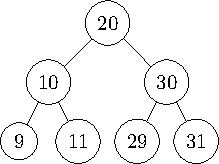
\includegraphics{lualatex/pa/8/binarysearchtree.pdf}
\end{highlight}

\paragraph{Linear}\label{par:linearbst}

For the linear search, we are counting how many steps it takes to reduce \(n\) to \(1\) by decrementing by \(1\).

\paragraph{Logarithmic}\label{par:logarithmicbst}

For the binary search tree, we are counting how many steps it take to reduce \(n\) to \(1\) by halving each time.

\subsubsection{Uses}\label{ssub:usesbst}

Often information lends itself to the tree structure automatically, some examples are:
\begin{itemize}
    \item Family trees
    \item Biology classification trees
    \item File systems
    \item Web addresses
\end{itemize}
However, data doesn't always fall into that structure, but we can force the data into that structure because of the algorithmic complexity gains.

\subsection{Basic Definitions}\label{sub:basic_definitions}

\begin{description}
    \item[Node] Each value on a tree
    \item[Edge] Edges connect two nodes together in one direction
    \item[Root] The very top node without any other nodes pointing to it
    \item[Path] The edges and nodes that you have to take to go from one node to another node
    \item[Children] All direct descendants of another node
    \item[Parent] The node that another node is connected to
    \item[Sibling] All nodes that are children of the same parent
    \item[Subtree] Any node and all of its descendants can form a subtree inside a larger tree
    \item[Leaf node] Nodes that have no descendants
    \item[Level] How many steps it is from the root
    \item[Height] The total number of levels on a tree
\end{description}

\subsection{Definition}\label{sub:definitiontree}

A tree is:
\begin{itemize}
    \item A \emph{set} of nodes
    \item A \emph{set} of edges that connect pairs of nodes
\end{itemize}
such that:
\begin{itemize}
    \item One node is the root node
    \item Every node (except root) is connected by an edge from only one other node (eg. Every node has one parent)
    \item There is a unique path from root to every node (comes from every node having one parent)
    \item A node can have any number of children, but a tree can only be called a \emph{binary tree} if each node has a maximum of two children.
\end{itemize}

\begin{note}
    A tree is a recursive data structure since every node of a tree can be considered the root of another sub tree.
    This recursive nature lends itself to recursive operations very well.
\end{note}

\section{Binary Trees and Balanced Binary Trees}\label{sec:binary_trees_and_balanced_binary_trees}

A binary tree is a linked data structure where each node has a \mintinline{text}{key} attribute, and three pointer attributes:
\begin{itemize}
    \item \mintinline{text}{node.p} points to the parent
    \item \mintinline{text}{node.left} points to the left child
    \item \mintinline{text}{node.right} points to the right child
\end{itemize}
Where the child or parent is missing (we are at the root, or there is only one child), we set the value to \mintinline{text}{NILL}.

\subsection{Balanced Binary Trees}\label{sub:balanced_binary_trees}

\begin{highlight}{A balanced binary search tree compared with an unbalanced binary tree}
    \begin{minipage}{0.45\linewidth}
        \centering
        A balanced binary tree

        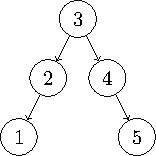
\includegraphics{lualatex/pa/8/balancedbst.pdf}
    \end{minipage}
    \hfill
    \begin{minipage}{0.45\linewidth}
        \centering
        An unbalanced binary tree

        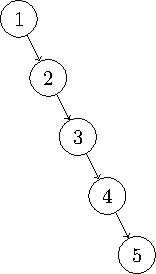
\includegraphics{lualatex/pa/8/unbalancedbst.pdf}
    \end{minipage}
\end{highlight}

A balanced tree is where the left and right subtrees of very node differ in height by no more than \(1\), making the total time complexity to traverse the tree \(O(\log n)\).

Where we have an extremely unbalanced tree, it is pretty much a linked list, so the time complexity is \(O(n)\)
\begin{note}
    Generally graph algorithms work better on a balanced tree.
\end{note}

\section{Traversing a Tree}\label{sec:traversing_a_tree}

When you traverse (or walk) a tree, you visit each node exactly one.
Where is no single obvious way to go through a tree like there was with a linked list.
There are two types of traversal:
\begin{description}
    \item[Breadth-first] We are most occasionally interested in going through each level at a time. Sometimes called \emph{level-order traversal}.
    \item[Depth-first] Most often we are interested in going down each branch before going down the next.
\end{description}

\subsection{Breadth First}\label{sub:breadth_first}

\begin{highlight}{The order of nodes visited in the breadth first traversal of a binary tree}
    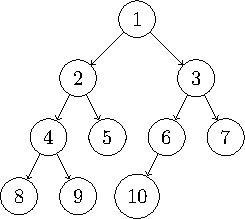
\includegraphics{lualatex/pa/8/breadthfirst.pdf}
\end{highlight}

Level traversal isn't always enough because it loses all of the ordering of the branches.

\subsubsection{Inorder Traversal}\label{ssub:inorder_traversal}

For an \emph{inorder traversal}, you first go to the leftmost leaf node, then you work your way back up to the top again recording the value of the parent (which wasn't technically visited on the way down), the left node, and then the right, so the order for any subtree is:
\begin{enumerate}
    \item Parent
    \item Left child
    \item Right child
\end{enumerate}
\begin{code}{text}
    INORDER(node)
        if node != NILL
            INORDER(node.left)
            print node.key
            INORDER(node.right)
\end{code}

\begin{highlight}{The order of nodes visited in the inorder traversal of a binary tree}
    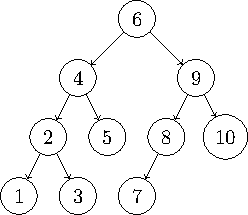
\includegraphics{lualatex/pa/8/inordertraversal.pdf}
\end{highlight}

\subsubsection{Preorder Traversal}\label{ssub:preorder_traversal}

For a \emph{preorder traversal}, you travel down through each left node recording the value each time, continuing until you reach then leaf node, then continue back up again visiting the right hand nodes, so the final order is:
\begin{enumerate}
    \item Parent
    \item Left child and all left hand descendants
    \item Right child and all right hand descendants
\end{enumerate}
\begin{code}{text}
    PREORDER(node)
        if node != NILL
            print node.key
            PREORDER(node.left)
            PREORDER(node.right)
\end{code}

\begin{highlight}{The order of nodes visited in the preorder traversal of a binary tree}
    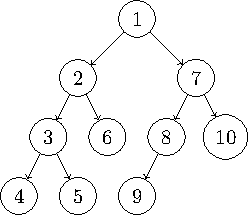
\includegraphics{lualatex/pa/8/preordertraversal.pdf}
\end{highlight}

\subsubsection{Postorder Traversal}\label{ssub:postorder_traversal}

For a \emph{postorder traversal}, you first go to the leftmost leaf node, then you work your way back up to the top again recording the value of the left node, then the parent node (which wasn't technically visited on the way down), and then the right, so the order for any subtree is:
\begin{enumerate}
    \item Left child
    \item Parent
    \item Right child
\end{enumerate}
\begin{code}{text}
    INORDER(node)
        if node != NILL
            INORDER(node.left)
            INORDER(node.right)
            print node.key
\end{code}

\begin{highlight}{The order of nodes visited in the postorder traversal of a binary tree}
    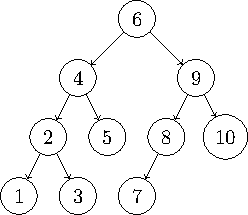
\includegraphics{lualatex/pa/8/postordertraversal.pdf}
\end{highlight}

\subsubsection{Recursive}\label{ssub:recursivetreetraversal}

Recursive algorithms are a very well known pattern that works by making a function call itself until some \emph{terminating condition} is met.
All of these depth first traversals are defined recursively because a tree is a recursive data structure.

\section{Binary Search Tree}\label{sec:binary_search_tree_operations}

A binary search tree is simply a binary tree where:
\begin{itemize}
    \item All nodes on the left subtree have keys smaller than \mintinline{text}{node.key}
    \item All nodes on the right subtree have keys larger than \mintinline{text}{node.key}
\end{itemize}
We can use an inorder traversal to get an ordered sequence.

Searching through a regular tree is time complexity \(O(n)\), but using a binary search tree means the time complexity is \(O(\text{height})\) which is roughly equal to \(O(\log n\) if the tree is perfectly balanced.
\begin{note}
    Remember: each step we eliminate half of the tree.
\end{note}

\section{Operations on Binary Search Trees}\label{sec:operations_on_binary_search_trees}

A binary search tree stored data in a specific structure, but to make the structure work for us, we need to define algorithms to perform operations on it (like we did for linked lists earlier).
The time complexity of all of the operations will be \(O(\text{height})\) where the height of a balanced tree is \(\log n\).

\subsection{Search}\label{sub:searchbst}

If the value we are looking for exists, we want to return a pointer to the while node, and return \mintinline{text}{NILL} otherwise.
\begin{code}{text}
    SEARCH(node, key)
        if node.key == key OR node == NILL
            return node
        if node.key > key
            return SEARCH(node.left)
        else
            return SEARCH(node.right)
\end{code}
Although this is a recursive function, we can also implement it recursively, which is usually more efficient.
\begin{code}{text}
    SEARCH-ITER(node, key)
        while node != NILL AND node.key != key
            if key < node.key
                node = node.left
            else
                node = node.right
\end{code}

\subsection{Insert}\label{sub:insertbst}

When we insert to a binary search tree, there are two steps:
\begin{enumerate}
    \item Create node
    \item Find an appropriate empty slot (remember it must still be a binary search tree).
    \item Insert the node to the position (remember to keep track of the \mintinline{text}{pnode} so that you can set \mintinline{text}{inode.parent} properly).
\end{enumerate}

\begin{code}{text}
    cnode = tree.root # current node
    pnode = NILL # parent node

    while cnode != NILL # leaf node has been found
        pnode = cnode
        if inode.key < cnode.key
            cnode = cnode.left
        else
            cnode = cnode.right

    inode.parent = pnode

    if pnode == NILL # We are at the root
        tree.root = inode
    elif inode.key < pnode.key
        pnode.left = inode
    else
        pnode.right = inode
\end{code}

\subsection{Minimum and Maximum}\label{sub:minimum_and_maximumbst}

Finding the minimum and maximums is very easy since we know that every node on the left of the parent is less than the parent, and that every node on the right is greater than the parent meaning that we can find the leftmost node for the minimum and rightmost node for the maximum.

\subsection{Linked List Implementation}\label{sub:linked_list_implementation}

A linked list is already a stack really, where the end pointer is points to the top pointer, since there is no traversal, we can say that the time complexity is \(O(1)\).
\begin{description}
    \item[PUSH] Insert to head
    \item[POP] Delete head, return value
\end{description}
\begin{note}
    Remember, we still need to prevent underflows
\end{note}

\section{Limitations of Binary Search Trees}\label{sec:limitations_of_binary_search_trees}

Each basic operation on a binary tree runs on \(O(h)\), but height varies as nodes are added or removed which can be problematic if the tree is not kept balanced (it could end up basically a linked list).
We should use \emph{self-balancing trees} where some extensions have been added to the basic binary search tree definition:
\begin{itemize}
    \item Red-black trees
    \item AVL trees
    \item B-trees
\end{itemize}
A common method to keep the tree balanced is to perform a rotation (basically tidying up / house keeping) after each deletion or insertion.
When we rotate, we find a pivot, then we swap to parent to the child so that the pivot is now the parent.

\section{Queue}\label{sec:paeightqueue}

For a queue, you enqueue and dequeue from the queue, where enqueuing adds nodes to the tail (the end), and dequeuing removes from the head (the front) of the list.

As with a stack, we have a ``peek'' called \mintinline{text}{FRONT-OF-QUEUE} that returns the front value, but doesn't remove it.
\mintinline{text}{SIZE-OF} returns the size, and \mintinline{text}{EMPTY} also returns whether the queue is empty or not.
\begin{note}
    Dequeuing an empty queue will still underflow.
\end{note}

If we were to implement a queue using an array, we have the head pointing to the start of the array, so when we dequeue from the queue, we have to move the head pointer forwards by one place, which unfortunately means we lose one place worth of space (we might even run out of space if the queue is empty).

We must use circular arrays to solve this problem, where we set our array indexes to \mintinline{text}{i=(i+1)%n} to loop back around to the start again.

\subsection{Conditions}\label{sub:queueconditions}

\begin{description}
    \item[Empty] The queue is empty is the head index equals the tail index.
    \item[Full] The queue is full if the head is one less than the tail (does equal pointers mean full or empty?). There is a special case for if the head set the start, then the tail will be \mintinline{text}{n-1} if full.
\end{description}
\begin{note}
    The condition we use for empty does mean that we lose a position in the queue.
    You can store \mintinline{text}{n-1} elements in a queue where \mintinline{text}{len(arr)=n}.
\end{note}

\subsection{Enqueue}\label{sub:enqueue}

\begin{code}{python}
    if self.queuefull:
        throw OverflowError
    else:
        self.arr[self.tail] = new
        self.tail = (self.tail + 1) % len(self.arr)
\end{code}

\subsection{Dequeue}\label{sub:dequeue}

\begin{code}{python}
    if self.queueempty:
        throw UnderfullError
    else:
        node = self.arr[self.head]
        self.head = (self.head + 1) % n
        return node
\end{code}

\subsection{Queue Empty}\label{sub:queueempty}

\begin{code}{python}
    return self.head == self.tail
\end{code}

\subsection{Queue Full}\label{sub:queue_full}

\begin{code}{python}
    return (
        (self.head == self.tail + 1) 
        or (self.head == 0 and self.tail == len(self.arr)-1)
    )
\end{code}

\subsection{Performance and Limitations}\label{sub:performance_and_limitations}

\begin{itemize}
    \item Space complexity is always \(O(n)\)
    \item The space must be defined before hand
\end{itemize}
\begin{note}
    For a linked list, we don't need to worry about any circular arrays, since we can just add or remove nodes whenever we want.
\end{note}

\section{Sequences}\label{sec:sequencespanine}

A sequence is similar to a set, except there is an order, we care about the relationship from one element to the next, and duplicates are allowed.
When we are looking at sequences, we will say that a relationship \emph{recurs} across elements (a recurring relationship between elements).
Once we get the starting value, we can use the recurring relation to recreate the entire sequence.

The idea of recurrence relations will link closely to the idea of recursive functions later on (and how to calculate their big \(O\) time).

One of the most important uses of recurrence relations is to provide solutions to certain ``counting problems'' like counting the steps in an algorithm, for example.

\subsection{Arithmetic Progression}\label{sub:arithmetic_progression}

An arithmetic progression is where a sequence has a common difference between terms, ie:
\[
    x = (\text{difference} \times n) + \text{offset}
\]
where \(x\) is the sequence element, \(\text{difference}\) is the space between the elements, and \(\text{offset}\) is the offset from \(0\) that the first element is.
All terms are real numbers.
This is usually written as \(x=a+nd\).

\begin{note}
    A good way to remember this, is that it creates a straight line graph, so is basically \(y=mx+c\).
\end{note}

\subsection{Geometric Progression}\label{sub:geometric_progression}

Here, there is a common ration between the terms, and not a common difference, ie:
\[
    x = \text{initial} \times \text{ratio}^{n}
\]
This can also be written as \(x=ar^{n}\).

\section{Recurrence Relations}\label{sec:recurrence_relations}

Sequences don't always have to have a relationship, but we don't care about these.
We can define a sequence by defining each item in terms of previous items (a recurrence relation), or we can use a formula to give the term at any position we want.

For a recurrence relation, we need to specify the relationship, as well as the first (or first few elements) of the sequence, for example we would say:
\begin{align*}
    a_0 = 0 \quad a_n = a_{n-1} + 2
\end{align*}
\begin{note}
    This means that \(\left\{a_n\right\}=0, 2, 4, 6, \ldots\). We need to specify that it's \(a_n\) and not just \(a\) since it represents the whole sequence and not just one value.
\end{note}

\section{Solving Recurrence Relations}\label{sec:solving_recurrence_relations}

If we take the recurrence relation:
\begin{align*}
    a_0 = 0 \quad a_n = a_{n_1}+2
\end{align*}
Then to find the \(50^{\text{th}}\) step, we would have to do \(50\) calculations (\(O(n)\)), but there is a better way.

Finding a formula for the \(n^{\text{th}}\) term of a recurrence relation is called solving the recurrence relation.
Such a formula is called a \emph{closed formula}.
\begin{enumerate}
    \item Start with the initial condition
    \item Work upwards until you reach \(a_n\) in terms of \(a_0\) and constants only
    \item Deduce the formula
\end{enumerate}

\section{Summations}\label{sec:summations}

A summation is represented by the \(\Sigma\) symbol:
\[
    \sum^{n}_{i=m} a_{i} = a_m + a_{m+1} + a_{m+2} + \dots + a_{n-1} + a_{n}
\]
A product is represented by the \(\Pi\) symbol:
\[
    \prod^{n}_{i=m} a_{i} = a_m \times a_{m+1} \times a_{m+2} \times \dots \times a_{n-1} \times a_{n}
\]
where \(n\) is the upper limit, \(m\) is the lower limit and \(i\) is the index.

\begin{note}
    We can also specify conditions for our sums:
    \[
        \sum_{j\in \{2, 5, 7, 10\} } a_j = a_2 + a_5 + a_7 + a_10
    \]
\end{note}

\section{Proof By Induction}\label{sec:proof_by_induction}

To prove a condition is true for any term in a sequence, we need to show:
\begin{enumerate}
    \item We can reach the first term
    \item We can reach any term
\end{enumerate}
To prove \(P(n)\), where \(n\in \Z^{+}\), show that \(P(1)\) is true (named the \emph{basis step}), then show that if \(P(k)\) is true, then \(P(k+1)\) is also true (named the \emph{inductive step}).
\begin{note}
    Here, \(P\) is a preposition or a statement that is either true or false.
\end{note}
The implication symbol looks like \(\to\), and the for all operator looks like \(\forall\), so we get \(P(k) \to P(k+1) \forall k\)
To complete the inductive step, we:
\begin{itemize}
    \item \textbf{Assuming} the inductive hypothesis that \(P(k)\) is true for any integer \(k\)
    \item \textbf{Show} that \(P(k+1)\) must be true by equating \(P(k) + (k+1)\) and \(P(k+1)\)
\end{itemize}

\subsection{Template}\label{sub:template}

\begin{itemize}
    \item State clearly what you want to prove, ie. \(P(n)\).
    \item Basic step (show that \(P(1)\) is true, or, in general \(P(b)\) is true)
    \item Inductive step
          \begin{itemize}
              \item State clearly \(P(k)\) -- ie. What we are assuming, also called the \emph{indicative hypothesis} -- and all values of \(k\)
              \item State clearly \(P(k+1)\) -- ie. What we want to prove
              \item Show that \(P(k+1)\) is true using the inductive hypothesis (\(P(k)\)). This usually means showing that \(\text{lhs} = \text{rhs}\), always start by manipulating \(\text{lhs}\), but keep an eye on \(\text{rhs}\) since this is where we want to end up.
          \end{itemize}
\end{itemize}

\section{Recursive Algorithms}\label{sec:recursionpaten}

Recursion is when a function calls itself.
We need to keep defining the problem as simpler versions of itself (that converge to the base case) until we get to the \emph{base case}.
It only works if:
\begin{itemize}
    \item There is a base case involved (aka terminating condition)
    \item Parameters to the function change toward the base case (we reduce the size of the data set, or the number we're working on) each time the function is called.
\end{itemize}

\subsection{Factorial Calculations}\label{sub:factorial_calculations}

Since
\begin{align*}
    5! & = 5 \times 4!                            \\
    5! & = 5 \times 4 \times 3!                   \\
    5! & = 5 \times 4 \times 3 \times 2!          \\
    5! & = 5 \times 4 \times 3 \times 2 \times 1! \\
    5! & = 5 \times 4 \times 3 \times 2 \times 1
\end{align*}
we can say that
\[
    n! = n \times (n-1)!
\]
Or
\begin{code}{python}
def factorial(n):
    if n == 1:
        return 1
    else:
        return n * factorial(n-1)
\end{code}

\subsubsection{Linear Sum Example}\label{ssub:linear_sum_example}

To find the first \mintinline{text}{n} elements of an array, the sum of all elements is the first element added to the sum of the rest.
\begin{code}{python}
def linear_sum(items, n):
    if n == 1:
        return n
    else:
        return linear_sum(items, n-1) + items[n-1]
\end{code}

\subsection{Recursion Trace}\label{sub:recursion_trace}

A graphical method to visualize an algorithms as a recursive algorithm executes.
\begin{itemize}
    \item Draw a box for each call
    \item Add an arrow from caller to callee
    \item Add an arrow from callee to caller showing the return value (we will often omit this)
\end{itemize}

\subsection{Linear and Binary Recursion}\label{sub:linear_and_binary_recursion}

\subsubsection{Linear Recursion}\label{ssub:linear_recursion}

A function calls itself at most once (the stopping case doesn't make a call to itself).
The trace looks like a straight line, and therefore the memory usage grows linearly as the number of steps increases.

\subsubsection{Binary Recursion}\label{ssub:binary_recursion}

This is where a function calls itself at most twice to solve two halves of the same problem.
The trace is a bit more complex because it looks like a binary tree now, instead of a straight. 
The Fibonacci sequence is a classic example of a binary recursive function:
\begin{highlight}{Fibonacci binary recursion}
    \begin{code}{python}
        def Fibonacci(n):
            if n <= 1:  # Base case
            # 0 and 1 are the two values n could be, these are base cases
                return n
            else:  # Binary recursion
                return Fibonacci(n-1) + Fibonacci(n-2)
    \end{code}
\end{highlight}

\subsection{Tail Recursion}\label{sub:tail_recursion}

Recursion has a cost since we need to keep track of the different function calls.
To overcome this, we can use iterations (ie. Loops), however we can also use tail recursion instead to reduce the memory usage of a function (which are also quite easy to convert to loops later, but the recursive one is usually easier to read).

\emph{Tail recursion} is where we make the recursive call be the last call of the function, so that when the child function is finished, the parent function is also finished, then this repeats all the way to the top of the recursive stack.
\begin{note}
    The speed benefit comes from us not having to load all (or even store) of the local variables back into memory again
\end{note}

\section{Searching}\label{sec:searching}

\begin{note}
    We are only doing membership testing here, because once we've found the index, we can just return the item.
    There is no difference in algorithm here.
\end{note}

\subsection{The Python Way}\label{sub:the_python_way}

Most algorithms will already be implemented in whatever language or libraries you are using, but doing that would make this course useless.

\begin{code}{python}
10 in [1, 2, 3, 4, 5, 6, 7, 8, 9, 10]
\end{code}

\subsection{Sequential Search}\label{sub:sequential_search}

The sequential search is an example of the \emph{incremental approach} to algorithm design, and is most useful when there is no order to the data.
The algorithm is simply moving from one side of an array to the other, and checking each element as you go.
\begin{code}{python}
    def search(elements, value):
        for element in elements:
            if element == value:
                return True
            
        return False
\end{code}

\subsubsection{Analysis}\label{ssub:sequntial_search_analysis}

If the item is present:
\begin{itemize}
    \item The base case is \(\Omega(1)\)
    \item The worst case is \(O(n)\)
\end{itemize}
If the item is not present:
\begin{itemize}
    \item The base case is \(\Omega(n)\)
    \item The worst case is \(O(n)\)
\end{itemize}

\subsection{Early Terminating Sequential Search}\label{sub:early_terminating_sequential_search}

If we know that the array is already sorted, we can assume that if the value of the current element is less than the target element, then we have gone past where the target element should be, and it therefore isn't in the array.
\begin{code}{python}
    deaf search(elements, value):
        for element in elements:
            if element == value:
                return True
            if element > value:
                return False
            
        return False
\end{code}

\subsubsection{Analysis}\label{ssub:analysis_early_terminating_search}

If the item is present:
\begin{itemize}
    \item The base case is \(\Omega(1)\)
    \item The worst case is \(O(n)\)
\end{itemize}
If the item is not present:
\begin{itemize}
    \item The base case is \(\Omega(n)\)
    \item The worst case is \(O(n)\)
\end{itemize}
\begin{note}
    This is exactly the same as before, since we have not changed the algorithm itself, we have only made the implementation slightly faster.
\end{note}

\subsection{Binary Search}\label{sub:binary_search_paeleven}

Binary search is only really useful if the array is sorted.
It works by splitting the array in two, then checking which half the target element should be in, then repeating until the element has been found.
\begin{enumerate}
    \item Look at the middle value
    \item If the target item is greater, discard the left half and the middle value, go to \(1\).
    \item If the target item is less, discard the right half and the middle value, go to \(1\).
    \item If the middle value is the search value, or if there are no values left, exit
\end{enumerate}

\begin{code}{python}
    def binary_search(elements, value):
        size = len(elements)
        mid = size // 2

        if size == 0:
            return False

        if elements[mid] == value:
            return True
        elif elements[mid] < value:
            binary_search(elements[mid+1:size], value)             
        else:
            binary_search(elements[0:mid], value)             
\end{code}

\subsubsection{Divide and Conquer}\label{ssub:divide_and_conquer}

Divide and conquer is where you split the problem into many smaller pieces, then solve those smaller pieces, and optionally (if the problem requires it), combine the pieces back together again.
A divide and conquer algorithm can usually be performed recursively.

\subsubsection{Analysis}\label{ssub:analysis_binary_search}

Since the problem size is halved each time, the time complexity is \(O(\log n)\).

\section{Sorting}\label{sec:sorting_pa_eleven}

\begin{note}
    Typically when we talk about sorting, we are talking about sorting in ascending order.
\end{note}

\subsection{Bubble Sort}\label{sub:bubble_sort_pa_eleven}

We covered this before already in \cref{sec:bubble_sort}, it's where we make multiple passes through the list comparing adjacent terms then moving the elements such that the larger ones bubble to the top.
The time complexity of a bubble sort is \(O(n^2)\).

\begin{code}{python}
    def bubble_sort(elements):
        n = len(elements)
        for outer in range(n-1, 0, -1):
            for i in range(outer):
                if (elements[i] > elements[i + 1]):
                    temp = elements[i]
                    elements[i] = elements[i + 1]
                    elements[i + 1] = temp
\end{code}

\subsection{Insertion Sort}\label{sub:insertion_sort}

We have to loop through the entire list (for each item), giving us \(n\) operations.
Then for each item of the list, we also have to place it in the correct position, which is also \(n\) operations in the worst case.
Therefore, insertion sort is also \(O(n^2)\) time complexity.

\begin{code}{python}
    def insertion_sort(elements):
        n = len(elements)
        for outer in range(1, n):  # all elements except first
            key = elements[outer]  # current element we're sorting
            inner = outer - 1  # sorted sub list ends at outer-1

            # Move key down through the sorted sub list, until it is placed correctly.
            while key < element[inner] and inner > 0:
                elements[inner] = elements[inner - 1]
                inner -= 1

            element[inner] = key
\end{code}



\chapter{Data Storage and Retrieval}\label{cha:data_storage_retrieval}

\etocsettocstyle{\section*{\contentsname}\par}{}
\etocsetnexttocdepth{subsubsection}
\localtableofcontents

\section{Course Introduction}\label{sec:dsr_course_introduction}

Throughout the course we will mainly be focusing on structured, relational databases which we will try to practice as much as possible practically.
During lectures, the first hour will generally be a practical session covering what was learned in the lecture section of the last lecture.
The second hour will be a lecture covering new content.

\subsection{Assessments}\label{sub:dsr_assessments}

\begin{description}
    \item[First coursework task] The first assessed task of the semester will be worth only \(5\%\) of the course grade and will be due \(2021-11-09\)
    \item[Second coursework task] The second of two assessed tasks will be worth \(20\%\) of the course and will be due on \(2021-11-19\)
    \item[Quizzes] Throughout the course, there will be several quizzes, these will be worth a total of \(5\%\)
         \item[Mid-semester class test] At roughly the half-way point of the course, we will have an in-class test on \(2021-11-24\) that will be worth \(10\%\) of the final grade
\end{description}

\begin{note}
    Everything in any lectures, coursework, or Moodle books will be examinable.
\end{note}

\subsection{Data, information, and knowledge}\label{sub:data_information_and_knowledge}

\begin{description}
    \item[Data] A structured representation of some raw data.
        This is just raw data and has no inherent meaning.
        Eg. \(52\) or \(14159\)
         \item[Information] This is also raw data, but it also has a meaning attached.
             Eg. ``The age is \(52\)'' or ``the user id is \(14159\).''
 \item[Knowledge] Information that can be ascertained from the information.
Eg. You could calculate the age category of the person, or you could calculate their sign up date from their user id.
\end{description}

\subsection{Problems in Data Management}\label{sub:problems_in_data_management}

We process \emph{lots} of data every day, and that amount will only grow into the future.
Databases are key to this, and are used in a variety of ways to aid and abet in the data processing pipeline.

For a database to be useful, we need it to be able to:
\begin{itemize}
    \item Store \emph{lots} of data
    \item Access all of our data (also query/search it)
        \item We don't want different versions of our data everywhere, so we want to avoid \emph{redundancy} because that can cause inconsistencies between copies of the same data.
            \item We want our database to be reliable, so that if there is one problem somewhere, the entire system doesn't break.
\end{itemize}

\subsection{Data Storage}\label{sub:data_storage}

Now that we've established that a database is the absolute best way of storing data, we need a tool to operate our database.
Any decent data storage tool must provide these features:
\begin{description}
    \item[Data Definition] This is the basic structure of a database
        \item[Data entry] We must be able to add new data to our database
            \item[Data editing] Data must be able to be edited after it has been added
                \item[Querying] We must be able to extract either a subset of our data or all of it back out of the database again.
                    \item[Persistence] Data must last in the database across different operations
\end{description}

To address these requirements we have a few choices:
\begin{description}
    \item[In memory-storage] This is the simplest, but it has no persistence, and requires that you re-enter data at the start of every runtime.
        \item[Files on disk] This is where each program handles it own representations of the data.
            This has the problem that it is very hard to have concurrent access to the same data (different programs will have different files), and to keep data consistent across different files.
            \item[Database management system] Sometimes this is also called a \emph{DBMS}.
                This is where all functions for storing data, as well as any related access functions (eg. performing calculations on the data) are in the same system.
                Usually the terms ``DBMS'' and ``Database'' are used interchangeably.
        \end{description}

\subsection{What is a database}\label{sub:what_is_a_database}

Inside of a database, data can be stored without any redundancy in a structured manner.
Individual users can be granted access to edit, add, delete, or access data and many users can access the same (or different) data at the same time.

\subsubsection{Types of database}\label{ssub:types_of_database}

\begin{description}
    \item[Hierarchical] This is almost exactly like a file system where data can only be accessed if you know the correct path to it.
        \item[Networked] This is very similar to a hierarchical database, except data is stored on a graph instead of a tree.
            \item[Relational] The main change here is that you can query data by field instead of by path now.
                \item[Object oriented] This was considered to be the ``next best thing'' in databases -- they didn't take off.
                    Data was stored on objects which could have properties or methods, instead of on tables.
                    \item[NoSQL] These are often still pretty much relational databases and use SQL underneath, but they just don't expose it to developers.
            \end{description}

\subsubsection{Relational Databases}\label{ssub:relational_databases}

A relational database stores data in a series of tables.
Tables are made up of a schema (a list of precisely defined fields) and information and can be linked together by a unique identifier.

\subsection{Database Operations}\label{sub:database_operations}

\subsubsection{View}\label{ssub:dsr_view}

Admins and users should be able to view different pieces of data in different formats.

\subsubsection{Manipulate}\label{ssub:manipulate}

Admins and users should be able to add, update, and delete different pieces of data.

\subsubsection{Query Types}\label{ssub:query_types}

\begin{description}
    \item[Exact Query] A query where there is one very exact, specific answer
        \item[Inexact Query] A query where there is no exact answer. Eg. What is the best restaurant?
\end{description}

\begin{note}
    Relational database can only handle exact queries.
\end{note}

\subsection{How do databases avoid redundancy?}\label{sub:avoiding_redundancy}

\begin{description}
    \item[Ambiguity] Databases make sure the same data is not stored somewhere else with with a different name.
        \item[Inconsistency] Databases make sure that any time data is changed, it is changed in all places it exists.
            \item[Wasted Effort] Databases avoid wasted effort by sharing data as much as possible.
\end{description}

\subsection{Controlled Concurrent Access}\label{sub:controlled_concurrent_access}

All users connected to a database should be able to see the same, correct data at the same time. Ie. One user update shouldn't cause incorrect data to be displayed to another user.
To avoid this, databases lock table rows using transactions to make concurrent database operations seem independent and sequential.



\chapter{Systems Programming}\label{cha:testing_and_software_improvements}

\etocsettocstyle{\section*{\contentsname}\par}{}
\etocsetnexttocdepth{subsubsection}
\localtableofcontents

\section{Pointers}\label{sec:c_pointers}

A memory address points to a location in memory where data can be stored.
When you pass a parameter to a function, the parameter data is copied to the new function (basically passing by value).

\begin{code}{c}
    void increment(int *n) { // Take an int pointer
        // The value at n's memory address is the value at n's memory address + 1
        *n = *n + 1;
    }

    int main() {
        int number = 6;
        increment(&number); // Pass the memory address of number
    }
\end{code}
\begin{note}
    \begin{description}
        \item[\&] Gets the address of a variable
        \item[*] Gets the value at an address
    \end{description}
    \begin{code}{c}
        *(&number) == number;
    \end{code}
\end{note}

\section{Pointers to Pointers}\label{sec:pointers_to_pointers}

\begin{code}{c}
    void increment_two(int *n) { // Take an int pointer
        // The value at n's memory address is the value at n's memory address + 1
        *n = *n + 1;
    }

    void increment_one(int **n) { // Pointer to a pointer to an int
        increment_two(*n); // Pointer to an int
    }

    int main() {
        int number = 6;
        int *pointer = &number; // Pointer to number
        increment(&pointer); // Pass pointer to pointer (double layer pointer)
    }
\end{code}

\section{Pointer Arithmetic}\label{sec:pointer_arithmetic}

\begin{code}{c}
    int main() {
        int a = 5;
        int b = 6;

        int *pointer_to_a = &a;
        *pointer_to_a = *pointer_to_a + 1; // Increments a

        // Increments the memory address after a, happens to be b here
        *(pointer_to_a + 1) = *(pointer_to_a + 1) + 1 
    }
\end{code}

\section{Arrays}\label{sec:c_arrays}

\begin{code}{c}
    int main() {
        // In memory, this is 5 consecutive memory locations
        int arr[5] = {1, 2, 3, 4, 5};

        // An array variable is a pointer to the start of a section of memory       
        // These are both "syntactic sugar" for each other
        int a = arr[2] // 3
        int b = *(arr+2) // 3
    }
\end{code}

\subsection{Appending To Arrays}\label{sub:c_appending_to_arrays}

\begin{code}{c}
    // An array variable is a pointer to a memory block.
    // We can also use arr[] instead of *arr too.
    void append(char *arr, char element, int index) {
        arr[index] = element
    }

    int main() {
        char arr[5] = {'a', 'b', 'c'}

        append(arr, 'd', 3)
        // Accessing data beyond the bounds of an array is undefined
        // behaviour and may do different things on different operating
        // systems
    }
\end{code}

\section{Nested Arrays}\label{sec:c_nested_arrays}

\begin{code}{c}
    int main() {
        int *a_value; // Pointer to an int
        int **some_value; // Pointer to a pointer to an int

        int arr_one[2] = {6, 5};
        int arr_two[2] = {2, 1};

        int **arrays[2] = {arr_one, arr_two};
        // arrays points to a memory location that points to
        // the start of arr_one
\end{code}

\section{Strings}\label{sec:c_strings}

\begin{code}{c}
    int main() {
        // C doesn't have strings, so we use character arrays instead
        char one_string[5] = {'a', 'b', 'c', 'd'};
        char another_string[5] = "abcd"; // Notice the double quotes

        printf("%s\n", another_string); 
        // How does the compiler know the length is 4 and not 5?
        // ASCII formatting has a NULL terminator that signifies the end, so:
        "abcd" == {'a', 'b', 'c', 'd', \0}.
        // You should almost never define a string as an array of characters.

        // Remember that trying to assign past the end of the array, eg:
        another_string = "abcde";
        // The behaviour is undefined, so ~anything~ could happen.
        
        // If you have pointers to data you are not meaning to access, 
        // you will get a segmentation fault
    }
\end{code}

\section{Segmentation Faults}\label{sec:segmentation_faults}

\begin{code}{c}
    int main() {
        int number = 6;
        *number;
        // We almost definitely can't access memory address 6, and it probably
        // has operating system code, so the operating system will just kill it.
        // This is a segmentation fault.
    }
\end{code}

\section{User Input}\label{sec:c_user_input}

\subsection{During Execution}\label{sub:during_execution}

\begin{code}{c}
    int main() {
        int age;

        // We want to update the variable, and not the value, so use a pointer.
        scanf("%d", &age); 
    }
\end{code}

\subsection{Prior To Execution}\label{sub:prior_to_execution}

\begin{code}{c}
    // argc is a conventional name that is the argument count.
    // argv is a conventional name that is an array of the argument texts.
    int main(int argc, char *argv[]) {
        int i;
        for (i = 0; i < argc; i++) {
            printf("%s\n", argv[i])
        }
    }
\end{code}

\section{Structures}\label{sec:c_structures}

\begin{code}{c}
    struct Address {
        int housenumber;
        char postcode[8];
    };

    int main() {
        struct Address connor = {124, "PA3 3BT"};
    };
\end{code}

\subsection{Type Definitions}\label{sub:type_definitions}

\begin{code}{c}
    typedef struct Address {
        int housenumber;
        char postcode[8];
    } address_t;

    typedef int age; // Just an alias really

    int main() {
        address_t connor = {124, "PA3 3BT"};

        connor.housenumber; // Value of housenumber
        &(connor.housenumber); // Memory address of housenumber
    }

    void getAddress(address_t *addressToSet) {
        addressToSet->housenumber; // -> follows a pointer, a . just gets the value.
    }
\end{code}

\section{Memory Allocation}\label{sec:memory_allocation}

\subsection{Stack Memory Allocation}\label{sub:stack_memory_allocation}

\begin{code}{c}
    #include <stdio.h>

    typedef struct Address {
        int housenumber;
        char postcode[8];
    } address_t;

    typedef int age;

    int main() {
        // This doesn't work since all getAddress()s will return the same
        // memory pointer since the stack frame will be created at the same place
        // (nothing else is allocated in between).
        // We end up with garbage data in *addrOne, *addrTwo, *addrThree
        address_t *addrOne = getAddress();
        address_t *addrTwo = getAddress();
        address_t *addrThree = getAddress();

        printf("You live at %d, %s\n", addrOne->housenumber, addrOne->postcode);
        printf("You live at %d, %s\n", addrTwo->housenumber, addrTwo->postcode);
        printf("You live at %d, %s\n", addrThree->housenumber, addrThree->postcode);
        // The solution is to have a completely separate space in memory that
        // the programmer is completely in control of, named heap memory
    }

    address_t *getAddress() {
        address_t addressToSet;

        scanf("%s", &addressToSet.housenumber);
        scanf("%s", &addressToSet.postcode);

        // Returning all of the data is potentially very slow
        // return addressToSet; 
        return &addressToSet; // Return pointer instead
    }
\end{code}

\subsection{Heap Memory Allocation}\label{sub:heap_memory_allocation}

\begin{code}{c}
    #include <stdlib.h>

    typedef struct Address {
        int housenumber;
        char postcode[8];
    } address_t;

    typedef int age;

    int main() {
        address_t *addrOne = getAddress();
        address_t *addrTwo = getAddress();
        address_t *addrThree = getAddress();

        printf("You live at %d, %s\n", addrOne->housenumber, addrOne->postcode);
        printf("You live at %d, %s\n", addrTwo->housenumber, addrTwo->postcode);
        printf("You live at %d, %s\n", addrThree->housenumber, addrThree->postcode);

        // The memory gotten by malloc will never be given back to the 
        // operating system unless we tell it to (memory leak).
        free(addrOne);
        free(addrTwo);
        free(addrThree);
    }

    address_t *getAddress() {
        // Get a pointer to heap allocated memory for the size of Address
        address_t * addressToSet = malloc(sizeof(address_t));
        // malloc can return a null pointer, so we should ideally
        // add some error handling (memory can be full, etc.).

        scanf("%s", &(addressToSet->housenumber));
        scanf("%s", &(addressToSet->postcode));

        return addressToSet;
    }
\end{code}

\section{Reallocation and Contiguous Allocation}\label{sec:realloc_and_calloc}

\subsection{Allocation and Reallocation}\label{sub:allocation_and_reallocation}

\begin{code}{c}
    int main() {
        int * number = malloc(sizeof(int)); // Pointer to the heap
        // Allocates array of length 5, hard to read, mistakes are easy
        int * number = malloc(sizeof(int) * 5); 
        // Allocates contiguous length of 5 integers, nice to read
        int * number = calloc(sizeof(int), 5); 
        int * number = malloc(sizeof(int));

        // To reuse a variable, we can free it, but we might not get the same
        // space, and it looks a bit nasty
        free(number);
        char * string[2] = calloc(sizeof(char), 2);

        // Or we can reallocate that memory instead, which is faster because 
        // it doesn't always need to free and allocate the whole memory space,
        // is very fast and is the recommender way of doing this.
        char * string[2] = realloc(number, sizeof(char) * 2);
    }
\end{code}

\subsection{Dangling Pointers}\label{sub:dangling_pointers}

\begin{code}{c}
    int main() {
        int * number = malloc(sizeof(int));
        free(number);

        // We still have the pointer address, but we don't own that memory
        // This is undefined behaviour, maybe causes a SegmentationFault.
        *number = *number + 6
        // There is no way around this, C is just doing what it's told.
    }
\end{code}

\subsection{Use After Free and Memory Leaks}\label{sub:use_after_free}

\begin{code}{c}
    #include <string.h>

    typedef struct address {
        int housenumber;
        char postcode[9];
    } address_t;

    address_t * createAddress(int housenumber, char * postcode) {
        // Allocate new space
        address_t * newAddress = malloc(sizeof(address_t));
        newAddress->housenumber = housenumber;
        // Not covered yet, we'll look at strings tomorrow
        strcpy(newaddress->postcode, postcode);
        newaddress->postcode = postcode;

        return newAddress
    }

    int main() {
        address_t * connorHouse = createAddress(123, "G11AA");
        connorHouse = createAddress(124, "G11AA"); // Value of connorHouse changes

        // We can no longer access the original connorHouse because we have lost
        // the address of it. We cannot call free() because we don't know what to free. 
        // When the program finishes, the operating system will free that memory. This
        // is a memory leak.

        // Free connorHouse
        free(connorHouse);

        // We can no longer access that memory, so the operating system kills the program
        // (undefined behaviour)
        printf("Connor: %d %s", connorHouse->housenumber, connorHouse->postcode);

        // This is a "double free" program, the operating system kills the program
        // (undefined behaviour)
        free(connorHouse);
    }
\end{code}


\section{Strings}\label{sec:strings_advanced}

\begin{code}{c}
    #include <string.h>

    typedef struct Person {
        char name[20];
        int age;
    } person_t;

    int main() {
        // This is problematic since we could accidentally overwrite the null terminator
        // which would make the string endless.
        char * text = "tom";
        text = "connor"

        person_t connor;

        char firstname[10] = "Connor";
        char surname[10] = "McLaughlin";

        // Basically equivalent to connor.name = firstname
        strcpy(&(connor.name), firstname);
        // Basically equivalent to connor.name += " " + surname
        strcat(&(connor.name), " ");
        strcat(&(connor.name), surname);

        int length = strlen(connor.name);
    }
\end{code}

\section{Nested Struct Instances}\label{sec:nested_struct_instances}

\begin{code}{c}
    #include <string.h>

    typedef struct Person {
        char name[20];
        int age;
        // person_t manager; // Endlessly recursive, we can't know the final size!!!
        person_t * manager; // We know exactly the size needed.
    } person_t;
\end{code}


\section{Parallelism}\label{sec:parallelism}

\subsection{Threads}\label{sub:threads_parallelism}

Threads are to be used when you want to run a piece of code many times

A thread shares a heap with all other threads, meaning they can access the memory space of each other, but they do have their own heap.
Because the threads all share the same heap, the operating system knows that the thread are linked and can kill them together.

Threads are quite lightweight since there is no new address space, and it is very cheap (and easy) to communicate between threads (basically managed by programmer).

\begin{code}{c}
#include <stdio.h>
#include <stdlib.h>
#include <pthread.h>

// We always need this same signature
// void * is a pointer to something whose type we don't know
void * entry(void *arg) {
    // arg is a void *, we need to cast to use it properly.
    int *threadNumber = (int *)arg;

    printf("My thread number is %d\n", *threadNumber);
    return NULL;
}

int main() {
    pthread_t threads[5];
    int arguments[5] = {1, 2, 3, 4, 5};

    int i;
    for (i = 0; i < 5; i++) {
        // thread pointer, thread arguments (not covered here),
        // function, function arguments (we can pass in structs
        // to get many values in.
        // pthread_create will update the thread with thread info.
        pthread_create(&threads[i], NULL, entry, &arguments[i])
    }

    for (i = 0; i < 5; i++) {
        // Wait for first result, then second, third, until all finished
        // Second argument is where to put result, 
        // we don't care about ours
        // We are not updating the thread, so we don't need a pointer.
        pthread_join(threads[i], NULL);
    }
}
\end{code}
\begin{note}
    Processes won't always print in order, if you want the answer from a thread in order, get the result from \mintinline{c}{pthread_join}, then print it.
\end{note}

\subsubsection{Accessing a stack value form another thread}\label{ssub:accessing_a_stack_value_form_another_thread}

\begin{code}{c}
#include <stdio.h>
#include <pthread.h>

void * increment(void * arg) {
    int *number = (int *)arg;
    *number = *number + 1;
    return NULL;
}

int main() {
    int x = 5;
    pthread_t thread;

    // Modify a value in main's stack
    pthread_create(&thread, NULL, increament, &x);

    // Without this, we might get 5 or 6
    pthread_join(thread, NULL);
    
    return 0;
}
\end{code}

\subsection{Process}\label{sub:process_parallelism}

A process is similar to a thread, except it is essentially its own program, and therefore has its own heap and stack.
Because they are basically separate programs, we can have processes that continue after the ending of its own program.

A process is quite heavy since the operating system has to do lots of processing to manage it (manage state, memory, etc), and communicate between them (IPC is slow).
\begin{note}
    A process is just a program, so can have its own threads too.
\end{note}

\subsection{Concurrency vs Parallelism}\label{sub:concurrency_vs_parallelism}

When we talk about parallelism, we are usually talking about threads and code running at the exact same time.
This can cause problems if the two pieces of code want to update the same memory address at the same time?

Concurrency is where two pieces of code are running at the same time, but individual operatations are interleaved with each other (like JavaScript promises), so we won't have to worry about accessing the same memory address.



\end{document}
